\documentclass[12pt,a4paper]{report}
\usepackage{vntex}
\usepackage[utf8]{inputenc}
\usepackage{a4wide,amssymb,epsfig,latexsym,multicol,array,hhline,fancyhdr}
\usepackage{booktabs}
\usepackage{amsmath}
\usepackage{bbm}
\usepackage{lastpage}
\usepackage[lined,boxed,commentsnumbered]{algorithm2e}
\usepackage{enumerate}
\usepackage{color}
\usepackage{graphicx,wrapfig}
\usepackage{subcaption}% Standard graphics package
\usepackage{tabularx, caption}
\usepackage{multirow}
\usepackage[framemethod=tikz]{mdframed}% For highlighting paragraph backgrounds
\usepackage{rotating}
\usepackage{graphics}
\usepackage{geometry}
\geometry{ left=30mm,right=20mm,top=20mm, bottom=20mm}
\usepackage{setspace}
\usepackage{listings}
\usepackage{float}
\restylefloat{table}
%%%%%%%%%%%%%%%%%%%%%%%%%%%%%%%%%%%%%%%%%%%%%%%%%%
\usepackage{titlesec}
\titleformat
{\chapter} % command
[display] % shape
{\Huge} % format
{\Large CHƯƠNG \ \thechapter} % label
{0.5ex} % sep
{
	\thispagestyle{empty}
    \rule{\textwidth}{1pt}
    \vspace{1ex}
    \centering
} % before-code
[
\newpage
] % after-code

%%%%%%%%%%%%%%%%%%%%%%%%%%%%%%%%%%%%%%%%%%%%%%%%%%
%use case
\usepackage{tikz-uml}
\tikzumlset{fill usecase=white}
%ERD Library
\usepackage{pdflscape}
\usepackage{tikz-er2}
\usepackage{adjustbox}
\usetikzlibrary{arrows,snakes,backgrounds}
\usetikzlibrary{positioning, shadows}
\tikzstyle{every entity} = [top color=white, bottom color=blue!30, 
                            draw=blue!50!black!100, drop shadow]
\tikzstyle{every weak entity} = [drop shadow={shadow xshift=.7ex, 
                                 shadow yshift=-.7ex}]
\tikzstyle{every attribute} = [top color=white, bottom color=yellow!20, 
                               draw=yellow, node distance=1cm, drop shadow]
\tikzstyle{every multi attribute} = [top color=white, bottom color=yellow!20, 
                               draw=yellow, node distance=1cm, drop shadow]
\tikzstyle{every relationship} = [top color=white, bottom color=red!20, 
                                  draw=red!50!black!100, drop shadow]
\tikzstyle{every isa} = [circle, top color=white, bottom color=green!20, 
                         draw=green!50!black!100, drop shadow]
\tikzstyle{line}=[draw]
%%%%%%%%%%%%%%%%%%%%%%%%%%%%%%%%%%%%%%%%%%%%%%%%%%

%%%%%%%%%%%%TreeView package%%%%%%%%%%%%%%%%%%
% \usetikzlibrary{trees}
% \tikzstyle{every node}=[draw=white,thick,anchor=west]
% \tikzstyle{selected}=[draw=red,fill=red!30]
% \tikzstyle{optional}=[dashed,fill=gray!50]
%%%%%%%%%%%%%%%%%%%%%%%%%%%%%%%%%%%%%%

\usepackage[unicode]{hyperref}
\setlength{\parskip}{0.5em}
\usepackage{indentfirst}
\usepackage{pgfgantt}
\hypersetup{urlcolor=blue,linkcolor=black,citecolor=black,colorlinks=true} 
\newcommand*\rfrac[2]{{}^{#1}\!/_{#2}}
\everymath{\color{black}}

\pagestyle{fancy}
\fancyhead{}
% \fancyhead[L]{
%  \begin{tabular}{rl}
%     \begin{picture}(25,15)(0,0)
%     \put(0,-8){
\includegraphics[width=8mm, height=8mm]{image/logo/hcmut.png}}
%    \end{picture}&
% 	\begin{tabular}{l}
% 		\textbf{\bf \ttfamily Trường Đại Học Bách Khoa TP.Hồ Chí Minh}\\
% 		\textbf{\bf \ttfamily Khoa Khoa Học và Kỹ Thuật Máy Tính}
% 	\end{tabular} 	
%  \end{tabular}
% }
\fancyhead[LE, RO]{
	Hệ thống Website du lịch Goz
}
\fancyfoot{} % clear all footer fields
% \fancyfoot[L]{\scriptsize \ttfamily Hệ thống thông tin Đoàn thanh niên - Hội sinh viên khoa Khoa học và Kỹ thuật Máy tính}
\fancyfoot[C]{
	Trang {\thepage}
	}
\renewcommand{\headrulewidth}{0.5pt}
\renewcommand{\footrulewidth}{0.3pt}


%%%

\usepackage{shorttoc}
\renewcommand*\contentsname{Contents (detailed)}
\setcounter{secnumdepth}{4}
\setcounter{tocdepth}{3}
\makeatletter
\newcounter {subsubsubsection}[subsubsection]
\renewcommand\thesubsubsubsection{\thesubsubsection .\@alph\c@subsubsubsection}
\newcommand\subsubsubsection{\@startsection{subsubsubsection}{4}{\z@}%
                                     {-3.25ex\@plus -1ex \@minus -.2ex}%
                                     {1.5ex \@plus .2ex}%
                                     {\normalfont\normalsize\bfseries}}
\newcommand*\l@subsubsubsection{\@dottedtocline{3}{10.0em}{4.1em}}
\newcommand*{\subsubsubsectionmark}[1]{}
\makeatother

\definecolor{dkgreen}{rgb}{0,0.6,0}
\definecolor{gray}{rgb}{0.5,0.5,0.5}
\definecolor{mauve}{rgb}{0.58,0,0.82}

\lstset{frame=tb,
	language=Matlab,
	aboveskip=3mm,
	belowskip=3mm,
	showstringspaces=false,
	columns=flexible,
	basicstyle={\small\ttfamily},
	numbers=none,
	numberstyle=\tiny\color{gray},
	keywordstyle=\color{blue},
	commentstyle=\color{dkgreen},
	stringstyle=\color{mauve},
	breaklines=true,
	breakatwhitespace=true,
	tabsize=3,
	numbers=left,
	stepnumber=1,
	numbersep=1pt,    
	firstnumber=1,
	numberfirstline=true
}
%%%%%%%%%%%%%%%%%%%%%%%%%%%%%%%%%%%%%%%%%%%%
%JavaScript
\lstdefinelanguage{JavaScript}{
  keywords={break, case, catch, continue, debugger, default, delete, do, else, finally, for, function, if, in, instanceof, new, return, switch, this, throw, try, typeof, var,let, const ,void, while, with},
  keywordstyle=\color{blue}\bfseries,
  ndkeywords={class, export, boolean, throw, implements, import, this},
  ndkeywordstyle=\color{darkgray}\bfseries,
  identifierstyle=\color{black},
  sensitive=false,
  comment=[l]{//},
  morecomment=[s]{/*}{*/},
  commentstyle=\color{purple}\ttfamily,
  stringstyle=\color{red}\ttfamily,
  morestring=[b]',
  morestring=[b]"
}

\lstset{
   language=JavaScript,
   backgroundcolor=\color{lightgray},
   extendedchars=true,
   basicstyle=\footnotesize\ttfamily,
   showstringspaces=false,
   showspaces=false,
   numbers=left,
   numberstyle=\footnotesize,
   numbersep=9pt,
   tabsize=2,
   breaklines=true,
   showtabs=false,
   captionpos=b
}
%%%%%%%%%%%%%%%%%%%%%%%%%%%%%%%%%%%%%%%%%%%%

\usepackage{tocloft}
\renewcommand{\cftchappresnum}{Chương }
\AtBeginDocument{\addtolength\cftchapnumwidth{\widthof{\bfseries Chương }}}

\pagenumbering{roman}
\begin{document}
\begin{titlepage}
\begin{tikzpicture}[remember picture, overlay]
  \draw[line width = 2pt,color=blue] ($(current page.north west) + (2.15cm,-2.15cm)$) rectangle ($(current page.south east) + (-2.15cm,2.15cm)$);
   \draw[line width = 1pt,color=black] ($(current page.north west) + (2.0cm,-2.0cm)$) rectangle ($(current page.south east) + (-2.0cm,2.0cm)$);
\end{tikzpicture}
\begin{center}
	\textbf{
	\large{
		ĐẠI HỌC QUỐC GIA THÀNH PHỐ HỒ CHÍ MINH \\
		TRƯỜNG ĐẠI HỌC BÁCH KHOA \\
		KHOA KHOA HỌC - KỸ THUẬT MÁY TÍNH 
	}}
\end{center}
%%%%%%%%%%%%%%%%%%%%%%%%%%%%%%%%%%%%%%%%%%%%%%%%%%%%%%%
\vspace{0.5cm}
\begin{figure}[h!]
\begin{center}
\begin{tabular}{cc}

\includegraphics[width=3.7cm]{image/logo/hcmut.png}     
\end{tabular}
\end{center}
\end{figure}
\vspace{0.5cm}
%%%%%%%%%%%%%%%%%%%%%%%%%%%%%%%%%%%%%%%%%%%%%%%%%%%%%%%
\begin{center}
\begin{tabular}{c}
\multicolumn{1}{c}{\textbf{{\Large LUẬN VĂN TỐT NGHIỆP ĐẠI HỌC}}}\\
~~\\
\hline
\\
\multicolumn{1}{c}{\textbf{{\Large XÂY DỰNG HỆ THỐNG WEBSITE  }}}\\
\textbf{{\Large DU LỊCH THÔNG MINH}}\\\\
\hline
\\
\end{tabular}
 \begin{tabular}{lll}
        \textbf{Ngành:} & \textbf{KỸ THUẬT MÁY TÍNH}\\
    \end{tabular}
\end{center}
%%%%%%%%%%%%%%%%%%%%%%%%%%%%%%%%%%%%%%%%%%%%%%%%%%%%%%%
\vspace{1cm}
\begin{table}[h!]
    \fontsize{15pt}{1}
    \centering
    \begin{tabular}{lll}
        \textbf{Hội đồng:} & \textbf{Khoa học máy tính}\\
        \textbf{GVHD:} & \textbf{TS Nguyễn Thị Ái Thảo }\\
        \textbf{GVPB:} & \textbf{Th.S Nguyễn Thanh Tùng}\\
\\
        \textbf{SVTH:} & \textbf{Đặng Hoàng Minh Trí (1513648)}\\
    \end{tabular}
\end{table}
\vspace{2.5cm}
\begin{center}
{\footnotesize TP. HỒ CHÍ MINH, THÁNG 2024}
\end{center}
\end{titlepage}

%%%%%%%%%%%%%%%%%%%%%%%%%%%%%%%%%%%%%%%%%%%%%%%%%%%%%%%%
\pagestyle{empty}
\begin{center}
\textbf{\LARGE Lời cam đoan}
\end{center}

Tôi xin cam đoan rằng đề tài luận văn tốt nghiệp: "Xây dựng hệ thống Website du lịch thông minh" là do tôi thực hiện dưới sự hướng dẫn của TS Nguyễn Thị Ái Thảo. Tất cả các tham khảo từ các công trình khác đều được ghi rõ trong mục "Tài liệu tham khảo". Nội dung của luận văn này chưa từng được công bố trước đây dưới bất kì hình thức nào. Nếu có bất kì sai phạm nào, tôi xin chịu hoàn toàn trách nhiệm trước Ban Chủ nhiệm Khoa và
Ban Giám hiệu Nhà trường.

\begin{flushright}
	Sinh viên thực hiện.
\end{flushright}
%%%%%%%%%%%%%%%%%%%%%%%%%%%%%%%%%%%%%%%%%%%%%%%%%%%%%%%%
\newpage
\begin{center}
	\textbf{\LARGE Lời cảm ơn}
\end{center}

Để hoàn thành luận văn tốt nghiệp này, em đã có 4 năm học tập tại trường đại học Bách khoa Thành phố Hồ Chí Minh, được sự giảng dạy tận tình của thầy cô trong trường, đặc biệt là các thầy cô trong Khoa Khoa học và Kỹ thuật Máy tính. Nay em xin gửi lời cảm ơn chân thành đến:

Trường Đại học Bách khoa Thành phố Hồ Chí Minh, nơi đã tạo cho em môi trường học tập tốt. Quý Thầy Cô Khoa Khoa học và Kỹ thuật Máy tính, những người đã truyền tri thức cùng tâm huyết của mình cho em vốn kiến thức quý báu trong suốt thời gian qua.

Em xin chân thành cảm ơn Cô Nguyễn Thị Ái Thảo đã tận tình chỉ dạy, hướng dẫn những kiến thức hữu ích và những ý kiến đóng góp chân thành để em có thể hoàn thành tốt luận văn tốt nghiệp này.

Cuối cùng em xin kính chúc toàn thể Quý Thầy Cô luôn dồi dào sức khỏe và thành công trong công việc.

Em xin chân thành cảm ơn!


\begin{flushright}
Sinh viên thực hiện.
\end{flushright}

%%%%%%%%%%%%%%%%%%%%%%%%%%%%%%%%%%%%%%%%%%%%%%%%%%%%%%%%
\newpage
\begin{center}
\textbf{\LARGE Tóm tắt báo cáo}
\end{center}

    Đề tài luận văn mà tôi thực hiện là "Xây dựng hệ thống Website du lịch thông minh". Trong quá trình thực hiện đề tài này, tôi đã thực hiện qua ba giai đoạn, cụ thể như sau:

\textbf{Giai đoạn 1: } Tiến hành khảo sát nhu cầu du lịch trên nhiều đối tượng đặc biệt là giới trẻ hiện nay .Từ đó, phân tích nghiệp vụ, tạo thành một quy trình cụ thể với đầu ra và đầu vào được xác định.

\textbf{Giai đoạn 2: } Đưa ra những vấn đề khó khăn và phương pháp khắc phục để đáp ứng nhu cầu người dùng  có một chuyến đi cụ thể, rõ ràng, rành mạch.

\textbf{Giai đoạn 3: } Đưa ra các phân tích và thiết kế hệ thống, tìm hiểu các kỹ thuật nền tảng triển khai. Tiến hành lựa chọn công nghệ phù hợp, xây dựng hệ cơ sở dữ liệu, sau đó xây dựng hệ thống trên nền tảng website. Mục tiêu là xây dựng hệ thống có khả năng đáp ứng với mọi đặc thù.

\textbf{Giai đoạn 4: } Triển khai thực tế và chạy thử nghiệm ....

    Báo cáo luận văn tốt nghiệp sẽ trình bày thông qua các nội dung chính sau đây:
    \begin{itemize}
        \item \textbf{Chương 1:} Tổng quan giới thiệu đề tài
        \item \textbf{Chương 2:} Nghiệp vụ và công nghệ sử dụng
        \item \textbf{Chương 3:} Phân tích và thiết kế hệ thống
        \item \textbf{Chương 4:} Hiện thực hệ thống
        \item \textbf{Chương 5:} Kiểm thử 
        \item \textbf{Chương 6:} Tổng kết và hướng phát triển
    \end{itemize}



%%%%%%%%%%%%%%%%%%%%%%%%%%%%%%%%%%%%%%%%%%%%%%%%%%%%%%%%
\newpage
\begin{center}
\textbf{\LARGE Thuật ngữ sử dụng}
\end{center}


\begin{center}
\begin{tabularx}{\textwidth}{|X|X|X|}
\hline
 \textbf{Từ viết tắt} & \textbf{Tên đầy đủ} & \textbf{Ý nghĩa} \\
 \hline
 Server, Server-side & & Máy chủ, Phía máy chủ \\  
 Client, Client-side & & Người dùng, Phía người dùng \\
 SQL & Structured Query Language & Ngôn ngữ truy vấn có cấu trúc \\
 NoSQL & Non-Relational Structured Query Language & Cơ sở dữ liệu phi quan hệ \\
 CSS & Cascading Style Sheets & Định nghĩa cách hiển thị cho HTML \\
 HTML & Hypertext Markup Language & Ngôn ngữ dùng để tạo trang web, ứng dụng web \\
 JavaScripts & & Ngôn ngữ lập trình phiên dịch. \\
 \hline
\end{tabularx}
\end{center}

\newpage
\tableofcontents
\newpage
\listoffigures
\newpage
\listoftables
\newpage
\clearpage
\pagestyle{fancy}

\pagenumbering{arabic}
%%%%%%%%%%%%%%%%%%%%%%%%%%%%%%%%%%%%%%%%%%%%%%%%%%%%%%%%
\chapter{\textbf{GIỚI THIỆU ĐỀ TÀI}}
\par{\textit{Trong chương này, tôi đưa ra những dẫn chứng về nhu cầu du lịch đặc biệt của giới trẻ trong đời sống hiện nay. Từ đó nêu ra lí do lựa chọn đề tài, tôi trình bày mục tiêu của đề tài và cuối cùng là ý nghĩa của đề tài.}}

\section{Giới thiệu đề tài và lý do chọn đề tài}
Du lịch được ghi nhận như là 1 sở thích, một hoạt động nghỉ ngơi mang đến sự tích cực của con người. Ngày nay, du lịch trở thành một nhu cầu không thể thiếu trong cuộc sống văn hoá, xã hội. Về mặt kinh tế, du lịch đã trỏ thành một trong những ngành kinh tế “hái tiền” lợi hại nhất của các nước. Mạng lứoi du lịch được thiết lập tất cả các quốc gia trên thế giới. \\
Ông bà ta còn có câu: \\
"	Đi 1 ngày đàng học 1 sàng khôn  "\\
Du lịch còn mang lại nhiều thông tin bổ ích, hiểu biết được nhiều kiến thức.Vì vậy để đưa du lịch đến gần tay hơn với mọi người, web du lịch đã nghĩ ra trên ý tưởng:\\
\par{\textit{"Thiết lập kế hoạch du lịch 1 cách chi tiết cho bản thân, nhóm, công ty…. Cho cách mục đi du lịch đâu? Ở đó làm gì? Ăn gi? uống gì? Địa điểm nào đẹp? Đi bao nhiêu ngày? Thời gian thực hiện các hoạt động trong ngày?  Tất cả đều nămf trong mục đăng kí kế hoạch đi đu lịch của bản thân, nhóm, công ty. Web sẽ hiện thực hoá suy nghĩ kế hoạch suông trong suy nghĩ thành những dữ liệu cụ thể( có đưa ra gợi ý). Ngoài ra bạn có thể chia sẻ plan mình cho những người muốn “rủ rê” đi cùng."}}

\section{Mục tiêu đề tài}
Với nhu cầu du lịch cao của mọi người hiện nay, đặc biệt là giới trẻ cùng với việc đã tham gia trải nghiệm  vào nhiều chuyến du lịch thực tế mà không có kế hoạch trước làm rất tốn thời gian, không chủ động trong sinh hoạt, du lịch .
\par{Website " Du lịch Goz " hướng đến việc khắc phục về việc đó. Người sử dụng có thể chủ động lên kế hoạch trước cho cá nhân hoặc nhóm: Đi đâu? Ăn gì? Trải nghiêm ở đâu? Di chuyển bằng phương tiện gì? Trong khung giờ như thế nào? }

\par{Mỗi bài thảo luận các thành viên bình luận, đóng góp ý kiến qua comment}
\par{Có thể đặt trước dịch vụ: thuê xe, thuê khách sạn, nhà hàng. Đánh giá dịch vụ đã sử dụng bằng điểm * và comment.}
\par{Sau khi đi du lịch sẽ có bài review về chuyến đi mà mình đã từng đi, dịch vụ từng ở, đánh giá nhận xét của bản thân về chuyến đi. Mỗi bài review đều có điểm tương tác thông qua cách chấm điểm trên thang 1-5 và bình luận}






% \section{Giới thiệu về đề tài và đặt vấn đề}
%     \par
%     Phòng Công tác chính trị Sinh viên có chức năng tổ chức thực hiện công tác giáo dục chính trị, tư tưởng cho cán bộ, viên chức và sinh viên toàn trường, đảm bảo đúng đường lối chính sách của Đảng, pháp luật của nhà nước; góp phần đào tạo sinh viên trở thành con người toàn diện có đạo đức, tri thức, sức khoẻ, thẩm mỹ và nghề nghiệp, trung thành với lý tưởng độc lập dân tộc và chủ nghĩa xã hội, dưới sự lãnh đạo của Hiệu trưởng và Đảng uỷ trường. Phòng Công tác Chính trị Sinh viên thực hiện các nhiệm vụ sau:
%     \begin{itemize}
%         \item Giáo dục chính trị - tư tưởng, đạo đức, lối sống và tổ chức các hoạt động rèn luyện cho sinh viên: triển khai các đợt sinh hoạt chính trị, học tập Nghị quyết, chủ trương của Đảng và chính sách pháp luật của nhà nước cho cán bộ, viên chức và sinh viên; nắm bắt tình hình diễn biến tư tưởng của sinh viên và đề xuất với Đảng uỷ, Hiệu trưởng có biện pháp tuyên truyền, giáo dục phù hợp và kịp thời.
%         \item Tổ chức thực hiện công tác đánh giá điểm rèn luyện theo năm học. 
%         \item Phối hợp với Đoàn Thanh niên, Hội Sinh viên, Ban liên lạc Cựu sinh viên tổ chức các hoạt động rèn luyện thân thể, xã hội, văn hoá, văn nghệ, thể dục thể thao.
%         \item Tổ chức tuần sinh hoạt công dân cho sinh viên vào đầu năm học.
%         \item Tổ chức thực hiện chế độ chính sách cho sinh viên: trợ cấp xã hội, miễn giảm học phí.
%         \item Phối hợp với các đơn vị, Đoàn Thanh niên, Hội sinh viên theo dõi và chịu trách nhiệm đề xuất công tác thi đua – khen thưởng, kỷ luật sinh viên với Hiệu trưởng.
%         \item Kiểm tra việc chấp hành quy chế học sinh - sinh viên nội trú, ngoại trú; kiến nghị xử lý các trường hợp vi phạm.
%     \end{itemize}
%     \par
%     Trong đề tài luận văn này sẽ tập trung giải quyết những vấn đề: Phối hợp với Đoàn Thanh niên, Hội Sinh viên tổ chức các hoạt động rèn luyện thân thể, xã hội, văn hoá, văn nghệ, thể dục thể thao. Xây dựng sàn hoạt động ngoại khóa sinh viên. Tổ chức thực hiện công tác đánh giá điểm rèn luyện, ngày CTXH theo năm học.
%     \par
%     \textbf{Kết luận chung: } Sinh viên khoa KH\&KT Máy tính nói riêng cũng như sinh viên trường Đại học Bách Khoa nói chung thực sự cần một hệ thống giải quyết được vấn đề đã được đề ra ở trên. Việc xây dựng hệ thống Phòng Công tác Chính trị Sinh viên là thực sự cần thiết. 

%     \section{Khó khăn, thử thách}
%     \begin{itemize}
%         \item Độ ổn định của hệ thống.
%         \item Tính bảo mật của hệ thống.
%         \item Lượng sinh viên sử dụng lớn.
%         \item Tính tiện lợi, đầy đủ các tính năng tuy nhiên vẫn dễ dàng trong sử dụng, vận hành.
%         \item Một hệ thống có thể áp dụng cho nhiều khoa với đặc điểm, cách hoạt động riêng.
%         \item Hỗ trợ được trên nhiều nền tảng khác nhau.
%     \end{itemize}
%     \section{Mục tiêu luận văn}
%     Mục tiêu của đề tài này là xây dựng một hệ thống (website, ứng dụng) Du lịch có đầy đủ các tính năng như sau:
%     % \begin{itemize}
%     %     \item Kênh thông tin cho người dùng có thể xem các bài viết, hoạt động, địa điểm du lịch đang nổi bật hiện nay.
%     %     \item Tính năng tạo kế hoạch, sự kiện trên hệ thống: người dùng có thể tạo các hoạt động một cách chi tiết trong ngày kèm theo một bài viết review đi kèm, các chức năng hỗ trợ ban truyền thông tạo, soạn thảo bài viết. Ngoài ra, hệ thống sẽ thực hiện được:
%     %     \begin{itemize}
%     %         \item Khi ban truyền thông, ban tổ chức đăng hoặc tổ chức sự kiện, hoạt động. Mỗi hoạt động, bài đăng sẽ phù hợp với những sinh viên khác nhau, hệ thống sẽ có nhiệm vụ gửi thông báo đến các sinh viên có nhu cầu cũng như gợi ý hoạt động cho sinh viên trên ứng dụng hoặc thông qua các kênh khác nhau.
%     %         \item Nhắc nhở sinh viên tham gia hoạt động khi hoạt động sắp diễn ra.
%     %         \item Cập nhật tình hình hoạt động của sinh viên cũng như là nhắc nhở sinh viên tham gia hoạt động.
%     %     \end{itemize}
%     %     \item Trợ lý sinh viên mỗi Khoa sẽ thực hiện được việc sắp xếp GVCN và thành phần ban cán sự lớp cho mỗi lớp trong mỗi năm học.
%     %     \item Khởi tạo bộ tiêu chí rèn luyện dành riêng cho mỗi Khoa dựa trên bộ tiêu chí chuẩn của Trường đưa ra. Mỗi khoa tạo, xoá, sửa, cập nhật các tiêu chí xét duyệt.
%     %     \item Tính năng cập nhật ngày CTXH và ĐRL sau mỗi sự kiện, hoạt động kết thúc.
%     %     \item Thực hiện công tác chấm điểm rèn luyện mỗi năm học online trên hệ thống. Sau đó được ban cán sự lớp và GVCN duyệt trước khi gửi kết quả về mỗi Khoa tổng hợp trước khi gửi về Trường.
%     % \end{itemize}

%     % Từ những mục tiêu tổng quát trên, nhóm nghiên cứu phân loại thành những mục tiêu cụ thể ứng với từng loại đối tượng người dùng trên một đơn vị, cụ thể như sau:
%     % \begin{itemize}
%     % \item 
%     % Các đối tượng quản lý:
%     % \begin{itemize}
%     %     \item 
%     %     Quản lý hệ thống.
%     %     \item 
%     %     Quản lý sự kiện, thêm, xoá, sửa, duyệt sự kiện.
%     %     \item
%     %     Quản lý các danh mục sự kiện để phân loại.
%     %     \item 
%     %     Cấu hình các sự kiện, thay đổi email để thông báo cho các sinh viên đăng ký tham gia sự kiện, tham gia sự kiện và cảnh báo sinh viên.
%     %     \item 
%     %     Tạo bản nháp sự kiện quá trình duyệt được trải qia 3 bước duyệt sự kiện bởi người có quyền, duyệt điểm rèn luyện, duyệt ngày CTXH có phù hợp với sự kiện đó hay không.
%     %     \item 
%     %     Cấu hình điểm rèn luyện, email nhắc nhở sinh viên phản hồi điểm rèn luyện nộp phiếu chấm điểm rèn luyện.
%     %     \item 
%     %     Tạo mới bộ tiêu chí cho mỗi Khoa, có thể copy từ Khoa khác hoăc từ bộ tiêu chí chuẩn của Trường. Thay đổi thêm, xoá sửa từng tiêu chí.
% %         \item 
% %         Vai trò ban cán sự lớp có nhiệm vụ xét duyệt lại các phiếu chấm điểm rèn luyện của các thành viên trong lớp của mình. Xem các phiếu chấm có đúng hay sai, có quyền chỉnh sửa điểm và để lại phản hồi.
% %         \item 
% %         Tương tự giáo viên cũng có thể duyệt điểm rèn luyện cho sinh viên của lớp chủ nhiệm. Ngoài ra còn có quyền phân cônn thành phần ban cán sự lớp. 
% %         \item 
% %         Trợ lý sinh viên mỗi Khoa sẽ có quyền gán GVCN và thành phần ban cán sự lớp cho mỗi lớp vào mỗi năm học cho Khoa. Tiếp nhận và xử lý phản hồi điểm rèn luyện của sinh viên.
% %         \item 
% %         Xuất ra danh sách điểm rèn luyện của Lớp, của Khoa.
        
% %     \end{itemize}
% %      \item 
% %     Đối tượng là sinh viên:
% %     \begin{itemize}
% %         \item 
% %         Xem các thông tin về điểm rèn luyện mỗi năm học.
% %         \item
% %         Thực hiện việc chấm điểm rèn luyện mỗi năm học.
% %     \end{itemize}
% % \end{itemize}
%     \section{Phạm vi đề tài}
%     Phạm vi các đối tượng mà đề tài hướng đến bao gồm:
%     \begin{itemize}
%         \item Người dùng ở mọi lứa tuổi, đặc biệt là giới trẻ từ 20 đến 30 tuổi.
%         \item Cộng tác viên khách sạn, homestay, quán ăn, .....
%     \end{itemize}

%%%%%%%%%%%%%%%%%%%%%%%%%%%%%%%%%%%%%%%%%%%%%%%%%%%%%%%%
\chapter{\textbf{NGHIỆP VỤ VÀ CƠ SỞ LÝ THUYẾT}}
\section{NGHIỆP VỤ}

Thông qua việc phân tích các yêu cầu của người dùng, nghiên cứu, ứng dụng các công nghệ hiện tại, đồng thời tham gia vào các chuyến du lịch Nhóm đã thống kê yêu cầu nghiệp vụ của ứng dụng và  xây dụng được một hệ thống thông tin Website du lịch như sau: 
\\
\\
\textbf{Bộ phận người dùng: } 
\begin{itemize}
    \item Người dùng không có tài khoản 
    \item Người dùng có tài khoản
\end{itemize}
\textbf{Người dùng không có tài khoản: }
Người dùng không có tài khoản chỉ sử dụng được một số chức năng cơ bản của hệ thống như : 
\begin{itemize}
    \item Xem thông tin kế hoạch du lịch có sẵn.
    \item Xem thông tin các tour du lịch.
    \item Xem thông tin các bài review, gợi ý địa điểm du lịch ở nơi họ muốn tới.
\end{itemize}
\textbf{Người dùng có tài khoản:} Sử dụng được tất cả chức năng của hệ thống và chính là nhóm đối tượng đề tài hướng tới. Để sỡ hữu tài khoản cho riêng cho cá nhân cũng như những trải nghiệm tốt nhất với hệ thống thì có một số quy trình chính như: 
\begin{quote}
    \textbf{Quy trình người dùng đăng kí tài khoản hệ thống: }
    \begin{itemize}
        \item Người dùng vào trang đăng kí tài khoản.
        \item Người dùng đăng ký tài khoản thông qua email.
        \item Thông tin tài khoản bao gồm email, username, họ và tên, ngày sinh, số điện thoại,.... trong đó thông tin họ và tên, email là bắt buộc.
    \end{itemize}
    \textbf{Quy trình người dùng đăng nhập vào hệ thống: }
    \begin{itemize}
        \item Người dùng vào trang đăng nhập và đăng nhập bằng tài khoản và mật khẩu đã đăng kí.
        \item Người dùng có thể đăng nhập thông qua googleID (gmail)
    \end{itemize}
    \textbf{Quy trình tạo kế hoạch cho chuyến đi: }
    \begin{itemize}
        \item Sau khi tham khảo các vài review cũng như các kế hoạch có sẵn thì người dùng có thể tiến hành tạo kế hoạch của mình.
        \item Người dùng chọn ngày khởi hành và khứ hồi.
        \item Người dùng chọn địa điểm đến.  
        \item Người dùng chọn chế độ cho kế hoạch "Private" và "Public".
        \item Người dùng nhấn "Khởi tạo" để chuyển sang giao diện thêm chi tiết hoạt động mỗi ngày cho chuyến đi.
        \item Người dùng chọn mốc thời gian cho các hoạt động của chuyến đi.
        \item Người dùng chọn khách sạn dừng chân cho chuyến đi, sau khi chọn type là "Hotel" thì sẽ có giao diện googlemap hiển thị các khách sạn nổi tiếng cũng như có lượt vote cao gợi ý cho khu vực người dùng muốn đến.
        \item Người dùng chọn địa điểm ăn uống, sau khi chọn type là "Eat n Drink" thì sẽ có giao diện googlemap hiển thị tất cả các quán ăn, các tiệm nước nổi bật cũng như có lượt vote cao trong khu vực đã chọn.
        \item Người dụng chọn các địa điểm du lịch thu thu hút đông khách du lịch ở địa phương thông qua type "Attraction".
        \item Sau khi đã chọn xong thì ngừời dùng nhấn "Add" để thêm các hoạt động chi tiết trong một ngày vào kế hoạch.
        
    \end{itemize}
     \textbf{Quy trình tạo bài review giới thiệu địa điểm du lịch:  }
     \begin{itemize}
         \item Sau khi đã trải nghiệm xong chuyến du lịch người dùng có thể viết bài review cho địa điểm mà mình đã đi.
         \item Người dùng chọn tạo bài blog.
         \item Người dùng chọn địa điểm đã đi 
         \item Người dụng chọn mốc thời gian đã đi
         \item Người dùng viết một bài blog cho những trải nghiệm thực của mình kèm thêm thông tin hình ảnh.
         \item Người dùng nhấn "Create" để bài blog cho mình.
         
     \end{itemize}
     \textbf{Quy trình người dùng gởi lời mời kết bạn: }
     \begin{itemize}
         \item Mỗi tài khoản người dùng có thể kết bạn và tương tác với nhiều người dùng khác.
         \item Người dùng nhấn "Friend" hoặc nhập tên người mình muốn kết bạn ở ô "Search" để xuất hiện giao điện những người mà mình muốn kết bạn.
         \item Người dùng nhấn "Add Friend" để gởi lời mời kết bạn đến đối phương.
         \item Người dùng nhấn "Delete" để xoá thông tin không phải người mình muốn kết bạn.
         
     \end{itemize}
     \textbf{Quy trình người dùng tương tác với lời mời kết bạn:  }
     \begin{itemize}
         \item Người dùng nhấn vào "Friend" để xem thông tin lời mời kết bạn mà các người dùng khác đã gởi cho mình.
        \item Người dùng nhấn "Accecpt" để đồng ý lời mời kết bạn.
        \item Người dùng nhấn "Decline" để từ chối lời mời kết bạn.
     \end{itemize}
     \textbf{Quy trình người dùng trò chuyện với nhau: }
     \begin{itemize}
         \item Người dùng nhấn vào "Messenger" hoặc biểu tượng Chat để mở giao diện trò chuyện.
         \item Người dùng chỉ có thể trò chuyện với bạn của mình.
         \item Người dùng có thể kiểm tra xem bạn bè có đang cùng hiện hữu không thông qua chấm xanh và đỏ ở góc hình avatar đối phương.
         \item Tại giao diện người dùng chọn người mình muốn trò chuyện, gõ thông tin cần nói là nhấn "Send". 
     \end{itemize}
     \textbf{Quy trình người dùng xem và tương các bài blog review: }
    \begin{itemize}
        \item Người dùng nhấn vào danh sách các bài Blog để xem danh sách các bài chú ý.
        \item Người dùng nhấn vào bài cần đọc.
        \item Tại giao diện blog người dùng có thể tương tác bằng cách thả like hoặc comment nhận xét.
    \end{itemize}
    \textbf{Quy trình người dùng xem các kế hoạch có sẵn: }
    \begin{itemize}
        \item Người dùng nhấn vào danh sách các kế hoạch có sẵn.
        \item Người dùng nhập vào ô tìm kiếm địa điểm mình muốn tham khảo và nhấn "Search".
        \item Giao diện sẽ xuất hiện tất cả các kế hoạch có sẵn về địa điểm mà người dùng muốn tìm kiếm.
        \item Người dùng chọn cho mình kế hoạch muốn xem.
    \end{itemize}
    
    \textbf{Quy trình người dùng chia sẻ kế hoạch của mình cho bạn bè: }
    \begin{itemize}
        \item Người dùng nhấn vào biểu tượng chia sẻ trên kế hoạch của mình.
        \item Hiển thị danh sách bạn bè muốn chia sẻ.
        \item Chọn bạn bè muốn chia sẻ và nhấn "Share"
        \item Hiển thị thông báo thành công.
    \end{itemize}
\end{quote}

   




\section{Mô hình phát triển website - Model View Controller}
\subsection{Mô hình phát triển website}
Kiến trúc Model-View-Controller (MVC) chia ứng dụng thành nhóm của ba thành phần chính: Models, Views, Controllers. Khi sử dụng khung mẫu lập trình này, yêu cầu (request) được chuyển cho Controller, Controller có trách nhiệm làm việc với Model để thực hiện yêu cầu của người dùng hoặc lấy dữ liệu từ cơ sở dữ liệu. Controller lựa chọn View để hiển thị ra với người dùng, cung cấp cho View những dữ liệu lấy từ Model.
Hình \ref{fig:mvcmodel} thể hiện những tương tác, truy vấn dữ liệu ở mỗi thành phần trong mô hình MVC, Controller sử dụng thông tin từ yêu cầu của người dùng để đưa ra những truy vấn dữ liệu thích hợp cho Model, từ đó dữ liệu được ghép chung với View để chuyển tới người dùng.
\begin{itemize}
    \item Model trong ứng dụng MVC thể hiện trạng thái của ứng dụng và các business rule. Các dữ liệu của công ty nên được tạo, lưu trữ, thay đổi dựa trên Model, dựa trên việc hiện thực tương tác, ràng buộc dữ liệu hợp lý để bảo đảm sự ổn định của ứng dụng.
    \item View có nhiệm vụ biểu diễn nội dung thông qua giao diện người dùng. Có thể nhúng trực tiếp dữ liệu vào HTML.
    \item Controller đóng vai trò trung gian giữa Model và View. Xử lí các yêu cầu của người dùng. Làm việc với Model và lựa chọn View để thể hiện nội dung một cách thích hợp.
\end{itemize}

Trong mô hình MVC, View chỉ hiển thị thông tin, Controller nhận, xử lý, phản hồi các yêu cầu, tương tác của người dùng. Controller là điểm khởi đầu, có trách nhiệm lựa chọn Model cần làm việc cùng, View cần để tạo nội dung.
\begin{figure}[H]
\centering
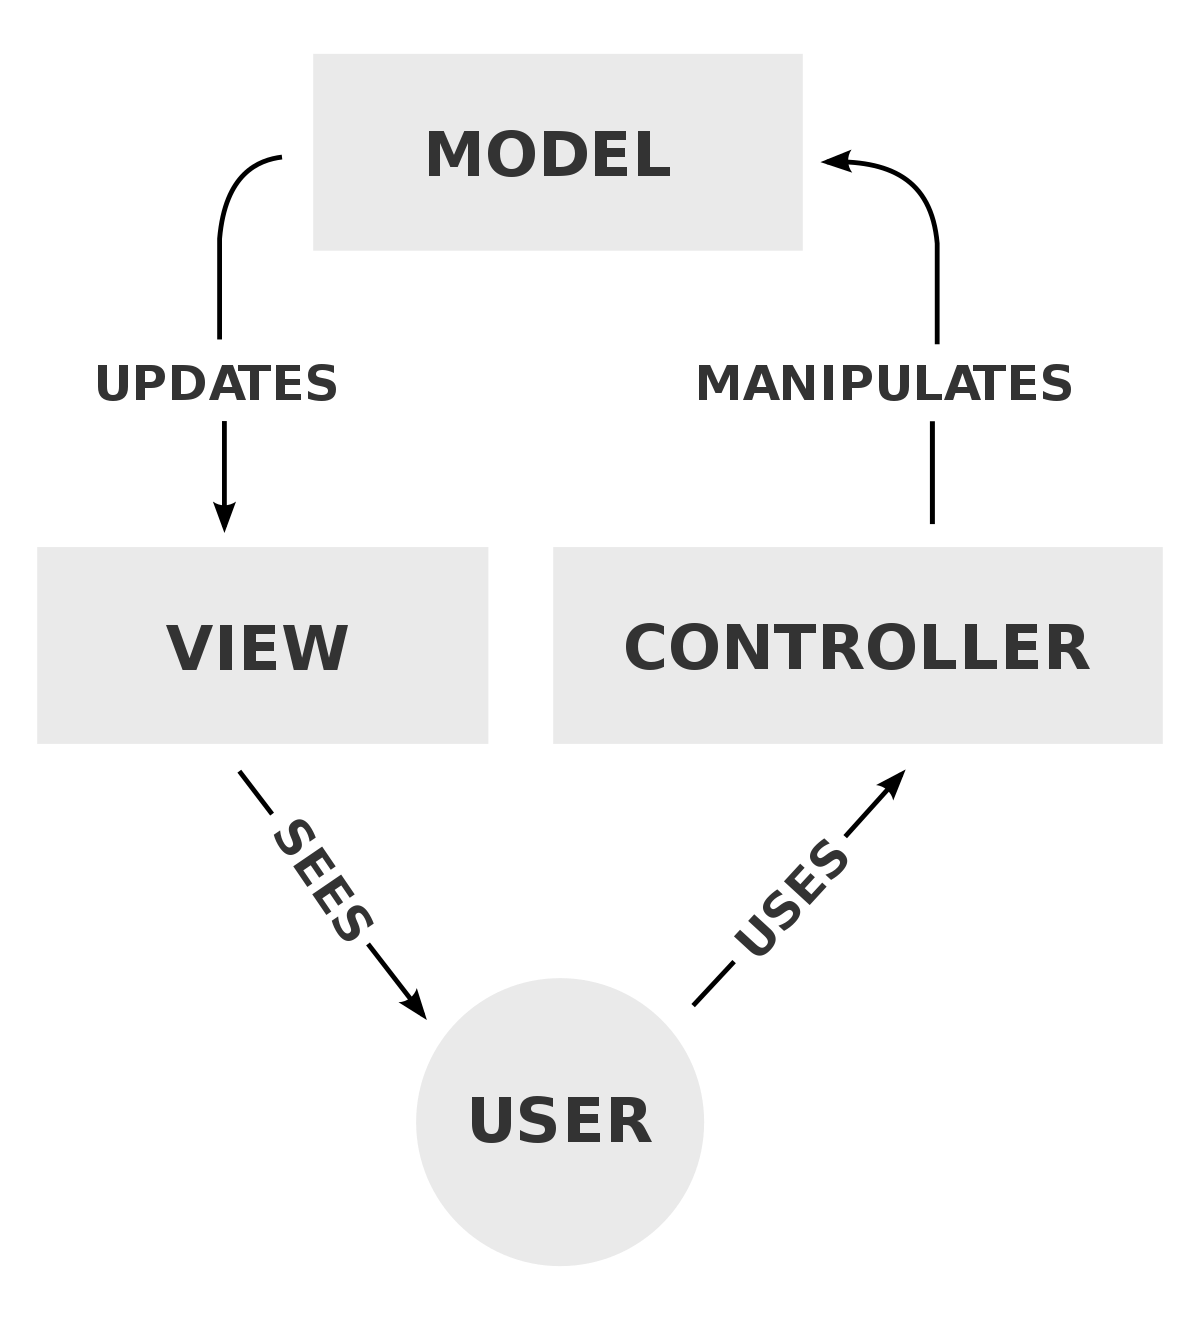
\includegraphics[width=10cm]{image/MVC.png}
\caption{Mô hình MVC}
\label{fig:mvcmodel}
\end{figure}

\section{Ứng dụng đa trang và ứng dụng đơn trang}
\subsection{Ứng dụng đa trang - Multi page application}
Ứng dụng đa trang hoạt động theo cách cơ bản nhất. Mọi thay đổi khi lấy dữ liệu, gửi dữ liệu lên máy chủ đều yêu cầu cập nhật lại toàn bộ trang bằng dữ liệu mới được gửi từ máy chủ, và hiện lên trình duyệt. Những trang này thường có kích thước lớn. Nhờ có AJAX, các ứng dụng đa trang hiện nay không cần truyền nhiều dữ liệu từ máy chủ đến trình duyệt. Chỉ cần làm mới những phần đi kèm với dữ liệu được thay đổi. Tuy nhiên, việc này trở nên phức tạp khi ứng dụng càng lớn.

Ưu điểm: 
\begin{itemize}
    \item Người dùng dể dàng thao tác trên ứng dụng cho các menu, điều hướng ít.
    \item Ứng dụng tốt các kỹ thuật SEO. Do ứng dụng chia thành nhiều trang, nên có thể tối ưu từng từ khóa cho mỗi trang.
\end{itemize}

Nhược điểm: 
\begin{itemize}
    \item Quá trình phát triển thường yêu cầu sự kết hợp chặt chẽ ở backend và frontend trong quá trình xử lý, nhận dữ liệu.
    \item Thời gian phát triển thường lớn khi so sánh với ứng dụng đơn trang.
\end{itemize}
\subsection{Ứng dụng đơn trang - Single page application}
Ứng dụng đơn trang tương tự như một ứng dụng ở trong trình duyệt, không yêu cầu quá trình tải lại trang khi sử dụng, nên giảm được thời gian chờ. Người dùng chỉ cần tải trang lần đầu, sau đó các nội dung sẽ được tải xuống bằng cách sử dụng JavaSript.
Ứng dụng đơn trang thường tách biệt giữa dữ liệu và HTML, CSS, trình duyệt sẽ trực tiếp hỗ trợ việc tạo nội dung. 


Ưu điểm: 
\begin{itemize}
    \item SPA nhanh, do hầu hết các tài nguyên (HTML, CSS, Scripts) được tải một lần trong suốt quá trình sử dụng ứng dụng. Chỉ có dữ liệu được truyền qua lại giữa trình duyệt và máy chủ.
    \item Quá trình phát triển thường đơn giản hơn. Do khi phát triển, lập trình viên không cần quan tâm đến việc tạo toàn bộ trang web ở phía máy chủ.
    \item SPA dễ dàng kiểm tra, kiểm lỗi hơn do phần lớn các trình duyệt (Chrome, FireFox,...) hỗ trợ tốt trong việc quan sát, debug, kiểm lỗi ngay trên trình duyệt.
    \item SPA có khả năng làm việc với bộ nhớ cục bộ, cache tốt. Nên hiệu quả hơn ứng dụng đa trang khi làm việc offline, do các tài nguyên chỉ cần tải xuống một lần.
\end{itemize}
Nhược điểm: 
\begin{itemize}
    \item Tải xuống thường lâu ở thời điểm đầu do lượng lớn tài nguyên cần tải xuống ở phía người dùng.
    \item JavaScript cần được cho phép chạy ở phía người dùng.
    \item Thường ít bảo mật hơn khi so sánh ứng dụng đa trang do XSS (Cross Site Scripting), cho phép kẻ tấn công có thể chèn mã phá hoại vào ứng dụng web tới người dùng khác.
    \item Rõ rỉ bộ nhớ có thể làm cho máy tính người dùng bị chậm đi đáng kể.
\end{itemize}

\subsection{Kết luận và lựa chọn}
Do khối lượng công việc, cũng như tính năng mà hệ thống ở luận văn cung cấp cho người dùng. Việc sử dụng SPA, ứng dụng đơn trang tỏ ra hiệu quả hơn. 
\begin{itemize}
    \item Việc chia nhỏ hệ thống ra thành nhiều phần nhỏ, quản lý, hiện thực ở SPA đơn giản hơn MPA.
    \item Hệ thống cần lưu trữ, chia sẽ nhiều dữ liệu giữa các tính năng, tác vụ. Do đó với SPA, có thể tận dụng bộ nhớ cục bộ (local storage) để hỗ trợ việc tương tác với người dùng.
    \item SPA đang được sử dụng rất nhiều, do đó có nhiều framework hỗ trợ, cộng đồng phát triển.
    \item Hệ thống được phát triển hỗ trợ cho hoạt động của đoàn khoa, do đó không cần chú trọng vào quản lý SEO.
\end{itemize}
Từ một số đặc điểm kể trên, nhóm quyết định lựa chọn mô hình ứng dụng đơn trang kết hợp với Model - View - Controller để phát triển hệ thống.
\section{Các nền tảng cho Javascript}
Khi lựa chọn xây dựng ứng dụng đa trang, có rất nhiều nền tảng, công nghệ hiện thực trên JavaScript hỗ trợ cho việc xây giao diện người dùng (front-end). Nâng cao hiệu suất công việc cũng như hỗ trợ quản lí mã nguồn tốt, ví dụ như Angular, ReactJS, VueJS. Sau đây nhóm sẽ giới thiệu, phân tích ưu nhược điểm một số công nghệ và đưa ra lựa chọn.

\subsection{AngularJs}
Angular là một framework được viết bằng TypeScript. Được phát triển bởi Google và được sử dụng trong Google AdWords, một dự án quan trọng của Google. Angular có cấu trúc cho các ứng dụng web động. Nó cho phép sử dụng HTML như là ngôn ngữ mẫu và cho phép mở rộng cú pháp của HTML để diễn đạt các thành phần ứng dụng một cách rõ ràng và súc tích. Hai tính năng cốt lõi: Data binding và Dependency injection của AngularJS loại bỏ phần lớn code thường phải viết. Nó xảy ra trong tất cả các trình duyệt, làm cho nó trở thành đối tác lý tưởng của bất kỳ công nghệ Server nào.
\subsection{VueJS}

\textbf{Vue.js} là một framework linh động (nguyên bản tiếng Anh: progressive – tiệm tiến) dùng để xây dựng giao diện người dùng (user interfaces). Khác với các framework nguyên khối (monolithic), VueJS được thiết kế từ đầu theo hướng cho phép và khuyến khích việc phát triển ứng dụng theo từng bước. Khi phát triển lớp giao diện (view layer), người dùng chỉ cần dùng thư viện lõi (core library) của VueJS, vốn rất dễ học và tích hợp với các thư viện hoặc dự án có sẵn. Cùng lúc đó, nếu kết hợp với những kĩ thuật hiện đại như SFC (single file components) và các thư viện hỗ trợ, VueJS cũng đáp ứng được dễ dàng nhu cầu xây dựng những ứng dụng một trang (SPA - Single-Page Applications) với độ phức tạp cao hơn nhiều.

\subsection{ReactJS}

\textbf{ReactJs} là một thư viện Javascript đang nổi lên trong những năm gần đây với xu hướng Single Page Application. Trong khi những framework khác cố gắng hướng đến một mô hình MVC hoàn thiện thì React nổi bật với sự đơn giản và dễ dàng phối hợp với những thư viện Javascript khác. Nếu như AngularJS là một Framework cho phép nhúng code Javascript trong code HTML thông qua các thược tính như ng-model, ng-repeat...thì với ReactJS là một thư viện cho phép nhúng code HTML trong code Javascript nhờ vào JSX, điều đó giúp dễ dàng lồng các đoạn HTML vào trong JS. Tích hợp giữa Javascript và HTML vào trong JSX làm cho các component dễ hiểu hơn. Một trong những điểm hấp dẫn của React là thư viện này không chỉ hoạt động trên phía client, mà còn được render trên server và có thể kết nối với nhau. React so sánh sự thay đổi giữa các giá trị của lần render này với lần render trước và cập nhật ít thay đổi nhất trên DOM. Nhờ đó ReactJS có hiệu năng tốt hơn những công nghệ hiện tại.

\subsection{Kết luận và lựa chọn}
Như đã đề cập ở trên, ReactJs là một Thư viện Javascript được tạo ra bởi sự cộng tác giữa Facebook và Instagram. Việc lựa chọn ReactJs là công cụ phát triển được dựa trên nhiều tiêu chí bao gồm hướng tiếp cận, trải nghiệm người dùng, thư viện hỗ trợ từ cộng đồng,... Điểm qua vài ưu điểm của ReactJs như sau:
\begin{itemize}
    \item ReactJS tạo ra cho chính nó DOM ảo – nơi mà các component thực sự tồn tại trên đó. Điều này sẽ giúp cải thiện hiệu suất rất nhiều. ReactJS cũng tính toán những thay đổi nào cần cập nhật lên DOM và chỉ thực hiện chúng. Điều này giúp ReactJS tránh những thao tác cần trên DOM mà nhiều chi phí.
    \item ReactJS giúp việc viết các đoạn code JS dễ dàng hơn: Nó dùng cú pháp đặc biệt là JSX (Javascript mở rộng) cho phép ta trộn giữa code HTML và Javascript. Ta có thể thêm vào các đoạn HTML vào trong hàm render mà không cần phải nối chuỗi. Đây là đặc tính thú vị của ReactJS. Nó sẽ chuyển đổi các đoạn HTML thành các hàm khởi tạo đối tượng HTML bằng bộ biến đổi JSX.
    \item Một trong những vấn đề với các ứng dụng đơn trang là tối ưu SEO và thời gian tải trang. Nếu tất cả việc xây dựng và hiển thị trang đều thực hiện ở client, thì người dùng sẽ phải chờ cho trang được khởi tạo và hiển thị lên. Điều này thực tế là chậm. Hoặc nếu giả sử người dùng vô hiệu hóa Javascript thì sao? ReactJS là một thư viện component, nó có thể vừa render ở ngoài trình duyệt sử dụng DOM và cũng có thể render bằng các chuỗi HTML mà server trả về. 
    \item Hiệu năng cao đối với các ứng dụng có dữ liệu thay đổi liên tục, dễ dàng cho bảo trì và sửa lỗi.
\end{itemize}

\section{Các thư viện cho ReactJS}
\subsection{Flux}
Flux là một kiến trúc mà Facebook sử dụng trong khi làm việc với React. Flux không phải là một \textbf{framework} hay một \textbf{thư viện (library)}. Nó đơn giản chỉ là một kiểu kiến trúc mới hỗ trợ thêm cho React, đồng thời xây dựng ý tưởng về luồng dữ liệu một chiều \textbf{(Unidirectional Data Flow)}.

\textbf{Cấu trúc của Flux:}
\begin{itemize}
    \item \textbf{Actions} - Làm nhiệm vụ truyền dẫn dữ liệu tới Dispatcher (được coi như các Helper Method)
    \item \textbf{Dispatcher} - Nhận thông tin từ Actions, truyền tải dữ liệu \textbf{(payload)} tới các nơi đã đăng ký nhận thông tin.
    \item \textbf{Stores} - Là nơi lưu trữ trạng thái và các logic của hệ thống, đây chính là nơi sẽ đăng ký nhận dữ liệu với Dispatcher.
    \item \textbf{Controller Views} - Chính là các React Components, làm nhiệm vụ nhận các trạng thái \textbf{(state)} từ \textbf{Stores} và truyền dữ liệu (dưới dạng \textbf{props}) cho các thành phần con.
\end{itemize}
\textbf{Mô hình hoạt động:}


\begin{figure}[H]
\centering
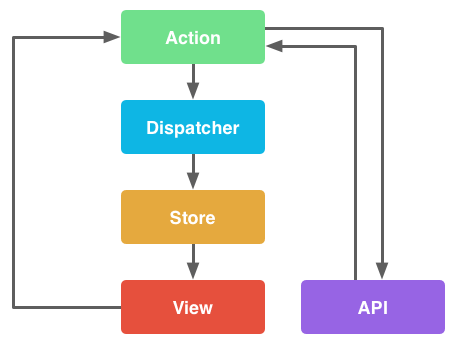
\includegraphics[width=10cm]{image/Redux-work-model.png}
\caption{Sơ đồ chung về quan hệ giữa các thành phần trong Flux}
\label{fig:redux_model}
\end{figure}
\textbf{Giải thích các thành phần trong hình \ref{fig:redux_model}:}
\begin{itemize}
    \item \textbf{Views} chính là thành phần làm nhiệm vụ hiển thị nội dung ứng dụng (thành phần này có nét tương đồng như thành phần \textbf{View} trong mô hình \textbf{MVC}).
    \item Khi người dùng tương tác với ứng dụng làm thay đổi trạng thái \textbf{(state)} của ứng dụng (Ví dụ như là các thao tác cơ bản trên dữ liệu: thêm, sửa, xóa), \textbf{View} sẽ thông qua \textbf{Action} gửi các thông tin thay đổi tới \textbf{Dispatcher} bao gồm:
    \begin{itemize}
        \item \textbf{action\_name}: tên của \textbf{Action} (Ví dụ: ADD\_USER).
        \item \textbf{action\_payload}: Nội dung muốn gửi (Ví dụ: firstname, lastname, email).
    \end{itemize}
    \item Sau khi nhận được thông tin từ \textbf{Action}, \textbf{Dispatcher} làm nhiệm vụ truyền tải \textbf{(broadcast)} nội dung nhận được tới các \textbf{Store} đăng ký lắng nghe sự kiện thay đổi từ trước đó.
    \item \textbf{Store} sau khi nhận thông tin, nó sẽ tiến hành việc cập nhật dữ liệu (Việc cập nhật dữ liệu này giống việc \textbf{setState} của Component).
    \item Sau khi cập nhật, \textbf{Store} bắn sự kiện xuống \textbf{View} để tiến hành cập nhật hiển thị cho người dùng.
    \item \textbf{API} giúp đỡ việc lấy dữ liệu từ Remote Server.
\end{itemize}


Sơ đồ trên đảm bảo luồng dữ liệu di chuyển trong Flux bắt buộc đi theo một đường nhất định.
\subsection{Redux}
Redux là một công cụ quản lý các trạng thái dự đoán được \textbf{(predictable state management tool)} cho các ứng dụng \textbf{Javascript}. Redux giúp bạn viết các ứng dụng hoạt động một cách nhất quán, chạy trong các môi trường khác nhau (client, server, và native) và dễ dàng kiểm thử.


\textbf{Cách thức Redux hỗ trợ ReactJS}


ReactJS được xây dựng theo một cách sao cho các \textbf{Components} đến việc quản lý nội bộ các \textbf{state} của chúng mà không cần bất kỳ một thư viện nào từ bên ngoài. ReactJS sẽ hoạt động tốt với các ứng dụng có ít component, nhưng khi ứng dụng trở lên lớn hơn thì việc quản lý các state được chia sẻ qua các component sẽ biến thành các công việc phức tạp.


Trong ReactJS, để truyền dữ liệu thông qua các \textbf{Component}, phải đảm bảo state luôn sống trong component cha, một \textbf{method} để cập nhật state trong chính component cha này và truyền cả state và method dưới dạng \textbf{props} đến các component con. Đây mới chỉ là cách thức truyền state trong các component cha - con, việc truyền state giữa các component có quan hệ cách xa nhau thì đó là một vấn đề lớn. Điều này khiến cho bộ phận quản lý state trong ứng dụng trở nên vô cùng phức tạp và Redux đã giải quyết được vấn đề đó.


\textbf{Cách thức hoạt động của Redux:}

Redux có \textbf{store} để lưu trữ toàn bộ \textbf{state} của ứng dụng. Bất kỳ component nào cũng có thể truy cập trực tiếp đến state được lưu trữ thay vì phải truyền theo \textbf{props} từ component này đến component khác! Redux có 3 thành phần chính: \textbf{Actions, Store, Reducers}
\begin{enumerate}
    \item \textbf{Actions}
    \begin{itemize}
        \item \textbf{Actions} đơn giản là các sự kiện, là cách thức gửi dữ liệu từ ứng dụng đến \textbf{store}. Những dữ liệu này có được từ sự tương tác của người dùng với ứng dụng, các lệnh gọi API hoặc từ các biểu mẫu \textbf{(form)}.
        \item \textbf{Actions} được gửi bằng cách sử dụng phương thức \textbf{store.dispatch()}. Các Actions phải có một thuộc tính \textbf{type} để diễn tả loại action, chúng cũng phải có một \textbf{payload} để chứa thông tin. Ví dụ như hình \ref{fig:redux-action-creator}
        \begin{figure}[H]
            \centering
            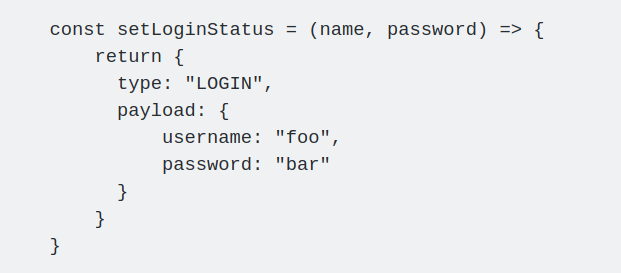
\includegraphics[width=10cm]{image/redux-action-creator.png}
            \caption{Một Action creator}
            \label{fig:redux-action-creator}
        \end{figure}
    \end{itemize}
    \item \textbf{Reducers}
    \begin{itemize}
        \item \textbf{Reducers} là các \textbf{hàm nguyên thủy}. Reducers lấy state hiện tại của ứng dụng, thực hiện một \textbf{action} và trả về một state mới. Những state này được lưu như những \textbf{Objects} và chúng định rõ cách state của một ứng dụng thay đổi trong việc phản hồi một action được gửi đến store.
    \end{itemize}
    \item \textbf{Store}
    \begin{itemize}
        \item \textbf{Store} lưu các \textbf{state} của ứng dụng và nó là \textbf{duy nhất} trong bất kỳ một ứng dụng Redux nào. Bạn có thể truy cập, cập nhật các state này.
        \item \textbf{Actions} thực hiện trên một state luôn luôn trả về một state mới. Vì vậy, state này là đơn giản và dễ đoán.
    \end{itemize}
\end{enumerate}


\subsection{Kết luận và lựa chọn}
\textbf{Flux} và \textbf{Redux} là 2 cái tên không xa lạ gì với cộng đồng \textbf{ReactJS}, chúng được sử dụng trong hầu hết các ứng dụng Javascript.


Kiến trúc của Flux tập trung giải quyết \textbf{'state changing'} rất hiệu quả. Tuy nhiên, Flux chỉ được Facebook giới thiệu như là một kiến trúc tổng quát ngoài ra họ không cung cấp cách hiện thực chi tiết nên ở ngoài cộng đồng hiện đã có rất nhiều phiên bản hiện thực lại, nổi tiếng nhất trong đó chính là Redux.


Điều làm cho Redux trở nên đặc biệt đó là REDUCER không bao giờ thay đổi state hiện tại của ứng dụng. Thay vào đó nó sẽ sao chép và trả về một state mới. Hướng tiếp cận này thường được thấy trong các ngôn ngữ hiện đại và thường được gọi là "state bất biến" \textbf{(“Immutable state”)}.


Tóm lại Flux và Redux là kiến trúc để quản lý state trong ứng dụng hiệu quả hơn. Flux là ý tưởng, kiến trúc tổng quát còn Redux là phiên bản được hiện thực lên từ Flux nên sẽ chi tiết hơn và sử dụng "immutable state" thay vì "mutable state". Chính vì điều này nên chúng ta sẽ thấy Redux khá phổ biến hơn là Flux và Redux sẽ thích hợp hơn với đề tài của nhóm.
\section{Bộ tiền xử lý}
\subsection{LESS}
LESS giúp viết các đoạn mã CSS đơn giản, ngắn gọn và hiệu quả hơn, đồng thời cũng dễ quản lý hơn bằng cách thêm vào CSS các thành phần động như biến, mixins, toán tử và hàm. LESS được phát triển bởi một lập trình viên người Đức là Alexis Sellier. Các thành phần cơ bản của LESS:
\begin{itemize}
	\item Biến được khai báo và sử dụng gán giá trị cho các thuôc tính. Ví dụ biến @color được sử dụng cho thuộc tính background-color trong class1
	\begin{verbatim}
	@color: #2d5e8b;
		.class1 {
		background-color: @color;
	}
	\end{verbatim}
	\item Mixins cho phép gắn toàn bộ thuộc tính của một class trong CSS vào trong class khác bằng cách thêm tên class này như một thuộc tính của class kia. Nó gần giống với biến, nhưng thay giá trị bằng toàn bộ các thuộc tính của class. Mixins cũng có thể được sử dụng như hàm, bằng cách truyền tham số.
	\begin{verbatim}
	.bordered {
		border-top: dotted 1px black;
		border-bottom: solid 2px black;
	}
	#menu a {
		color: #111;
		.bordered;
	}
	\end{verbatim}
\end{itemize}

\subsection{SASS}
    \begin{figure}[H]
        \centering
        
\includegraphics[width = 7cm]{image/sass-logo.png}
        \caption{SASS (Syntactically Awesome StyleSheets)}
        \label{fig:sass_logo}
    \end{figure}
    SASS (Syntactically Awesome StyleSheets) là một phần mở rộng của CSS, nó giúp chúng ta sử dụng biến (variables), quy tắc xếp chồng (nested rules), mixins, thừa kế (selector inheritance), hàm (functions), ... và hoàn toàn tương thích với cú pháp của CSS.
    
\subsection{Các đặc tính của SASS}
    \begin{itemize}
        \item Hoàn toàn tương thích với CSS.
        \item Mở rộng ngôn ngữ như các biến (variable), mixins, hàm (function), ...
        \item Nhiều function hữu ích cho các thao tác với màu sắc và các giá trị khác.
        \item Các đặc tính nâng cao như các control directive.
        \item Có cấu trúc, tùy biến đầu ra. SASS có hai định dạng file là *.sass và *.scss. Và cách viết của hai định dạng này cũng là khác nhau (nhưng các control directive, function thì có cùng một ý nghĩa).
    \end{itemize}
\subsection{@-Rules và Directives}
    \begin{itemize}
        \item @import\\
        Cho phép import các rule, style, biến, mixins, functions, ... từ một file SASS khác. Và nó sẽ được gộp lại thành một file khi xuất ra file CSS. Directive @import nhận một chuỗi là tên file sẽ được import. Mặc định, khi tên file không có phần mở rộng (extension), thì nó sẽ ưu tiên tìm file có phần mở rộng là *.scss và *.sass
        \begin{figure}[H]
            \centering
            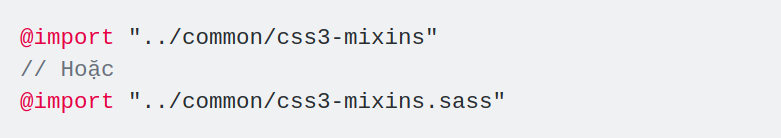
\includegraphics[width = 10cm]{image/sass-import.png}
            \caption{Ví dụ về @import}
            \label{fig:sass_import}
        \end{figure}
        \item @extend\\
        Cho phép bạn thừa kế các property của một class khác.
        \begin{figure}[H]
            \centering
            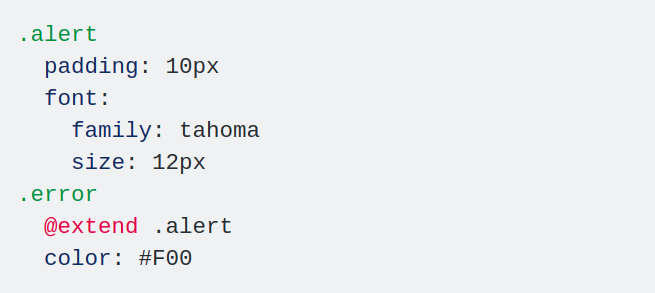
\includegraphics[width = 10cm]{image/sass-extend.png}
            \caption{Ví dụ về @extend}
            \label{fig:sass_extend}
        \end{figure}
        \item @each\\
        Giúp bạn duyệt một danh sách các giá trị, được dùng trong trường hợp phải viết một số lệnh giống nhau, nhưng chỉ khác chút về giá trị của thuộc tính.
        \begin{figure}[H]
            \centering
            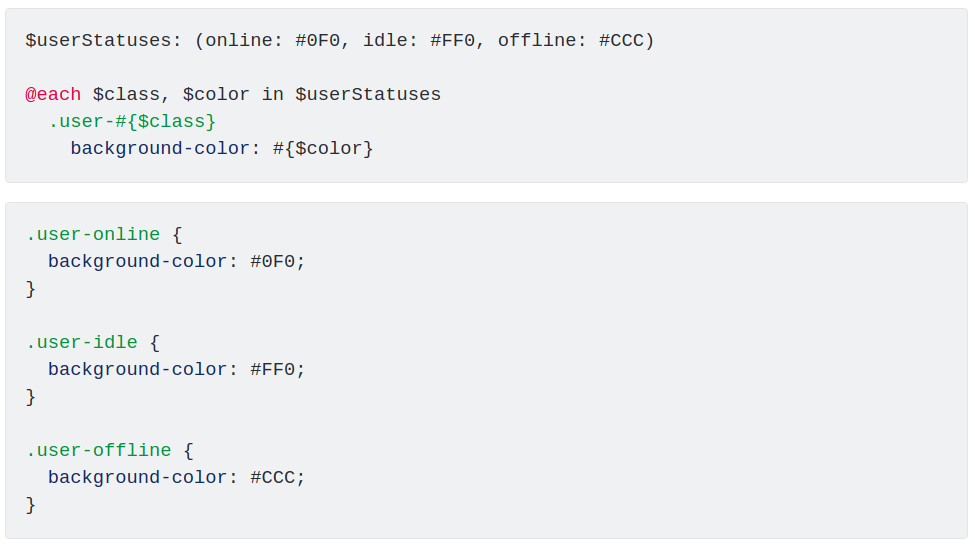
\includegraphics[width = 0.9\linewidth]{image/sass-each.png}
            \caption{Ví dụ về @each}
            \label{fig:sass_each}
        \end{figure}
        \item @mixin\\
        Giúp bạn định nghĩa một khối các style có thể được sử dụng lại nhiều lần. Trong SASS, ngoài @mixin còn @function, về bản chất nó giống nhau. Nhưng khác một chỗ, @mixin không trả về (@return) giá trị nào cả, còn @function thì luôn phải trả về một giá trị.
        \item @include\\
        Dùng để gọi các @mixin (trong file *.scss).
        \item @content\\
        Giúp bạn lấy toàn bộ nội dung của một khối để đưa vào @mixin.
    \end{itemize}
    
\section{Phía Server}
\subsection{Java}
\begin{enumerate}
    \item \textbf{Java}
    \begin{figure}[H]
        \centering
        
\includegraphics[width = 8cm]{image/java-logo.jpeg}
        \caption{Java Backend}
        \label{fig:java_logo}
    \end{figure}
    \begin{itemize}
        \item Java là một ngôn ngữ lập lập trình, được phát triển bởi \textbf{Sun Microsystem} vào năm 1995, là ngôn ngữ kế thừa trực tiếp từ C/C++ và là một ngôn ngữ lập trình hướng đối tượng.
        \item Ngày nay Java được sử dụng với các mục đích sau:
        \begin{itemize}
            \item Phát triển ứng dụng cho các thiết bị điện tử thông minh, các ứng dụng cho doanh nghiệp với quy mô lớn.
            \item Tạo các trang web có nội dung động (web applet), nâng cao chức năng của server.
            \item Phát triển nhiều loại ứng dụng khác nhau: Cơ sở dữ liệu, mạng, Internet, viễn thông, giải trí, ...
        \end{itemize}
    \end{itemize}
    \item \textbf{Những đặc điểm cơ bản của Java}
    \begin{itemize}
        \item Đơn giản và quen thuộc: Vì Java kế thừa trực tiếp từ C/C++ nên nó có những đặc điểm của ngôn ngữ này, Java đơn giản vì mặc dù dựa trên cơ sở C++ nhưng Java đã được lược bỏ một cách cẩn thận các tính năng khó nhất của của C++ để làm cho ngôn ngữ này dễ sử dụng hơn.
        \item Hướng đối tượng và quen thuộc.
        \item Mạnh mẽ (thể hiện ở cơ chế tự động thu gom rác - Garbage Collection) và an toàn.
        \item Kiến trúc trung lập, độc lập nền tảng và có tính khả chuyển (Portability).
        \item Hiệu suất cao.
        \item Máy ảo (biên dịch và thông dịch).
        \item Phân tán.
        \item Đa nhiệm: Ngôn ngữ Java cho phép xây dựng trình ứng dụng, trong đó nhiều quá trình có thể xảy ra đồng thời. Tính đa nhiệm cho phép các nhà lập trình có thể biên soạn phần mềm đáp ứng tốt hơn, tương tác tốt hơn và thực hiện theo thời gian thực.
    \end{itemize}
\end{enumerate}

\subsection{NodeJS}
\begin{enumerate}
    \item \textbf{Nodejs}
    \begin{figure}[H]
        \centering
        
\includegraphics[width = 6cm]{image/nodejs-logo.png}
        \caption{NodeJS backend}
        \label{fig:nodejs_logo}
    \end{figure}
    \begin{itemize}
        \item \textbf{NodeJS} là một \textbf{nền tảng (Platform)} phát triển độc lập được xây dựng ở trên \textbf{Javascript Runtime} của Chrome mà chúng ta có thể xây dựng được các ứng dụng mạng một cách nhanh chóng và dễ dàng mở rộng.
        \item NodeJS được xây dựng và phát triển từ năm \textbf{2009}, bảo trợ bởi công ty Joyent, trụ sở tại California, Hoa Kỳ.
        \item Phần lõi bên dưới của NodeJS được viết hầu hết bằng C++ nên cho tốc độ xử lý và hiệu năng khá cao.
        \item Nodejs tạo ra được các ứng dụng có tốc độ xử lý nhanh, thời gian thực.
        \item Nodejs áp dụng cho các sản phẩm có lượng truy cập lớn, cần mở rộng nhanh, cần đổi mới công nghệ, hoặc tạo ra các dự án Startup nhanh nhất có thể.
    \end{itemize}
    \item \textbf{Những lợi ích mà NodeJS mang lại}
    \begin{itemize}
        \item Các ứng dụng NodeJS được viết bằng Javascript, ngôn ngữ này là một ngôn ngữ khá thông dụng.
        \item NodeJS chạy đa nền tảng phía Server, sử dụng kiến trúc hướng sự kiện Event-driven, cơ chế non-blocking I/O làm cho nó nhẹ và hiệu quả.
        \item Có thể chạy ứng dụng Nodejs ở bất kỳ đâu trên máy Mac – Window – Linux, hơn nữa cộng đồng NodeJS rất lớn và hoàn toàn miễn phí, các package đều hoàn toàn miễn phí.
        \item Các ứng dụng NodeJS đáp ứng tốt thời gian thực và chạy đa nền tảng, đa thiết bị.
    \end{itemize}
\end{enumerate}
\subsection{Kết luận và lựa chọn}
\textbf{Java} được sử dụng trong các lĩnh vực công nghệ, chính phủ, tài chính, y tế, bảo hiểm, giáo dục, sản xuất, quốc phòng, ...


Điểm trừ của Java đó là tốc độ chậm, có rất nhiều config. Trong khi NodeJS lại làm tốt phần việc này. Với tính chất của đề tài là tiếp cận với nhiều đối tượng khác nhau và yêu cầu lượng truy cập lớn hơn sau mỗi năm, hơn nữa, đề tài này cần có khả năng mở rộng cao để phát triển hơn trong tương lai thì NodeJS mang lại nhiều thuận lợi và đáp ứng nhu cầu hơn cả.

Trong câu chuyện thay đổi của PayPal, NodeJS sử dụng ít hơn 33\% dòng mã và ít hơn 40\% tệp so với ứng dụng dựa trên Java trước đó, hơn nữa NodeJS nhân đôi số lượng request được cung cấp mỗi giây và giảm 35\% thời gian response trung bình.


Khi hiện thực bằng NodeJS, máy chủ chỉ phản ứng khi xảy ra sự kiện và môi trường không chặn. Điều đó làm cho NodeJS trở nên nhẹ và hiệu quả, hoàn hảo cho các ứng dụng thời gian thực sử dụng nhiều dữ liệu. (Trong đề tài là chức năng điểm danh tham gia sự kiện của sinh viên)
\subsection{Framework ExpressJS}
\begin{enumerate}
    \item \textbf{ExpressJS}
    \begin{figure}[H]
        \centering
        
\includegraphics[width = 10cm]{image/express-js.jpg}
        \caption{ExpressJS framework}
        \label{fig:express_JS_framework}
    \end{figure}
    \begin{itemize}
        \item \textbf{ExpressJS} là một \textbf{Framework}, có tính linh hoạt và được xây dựng trên nền tảng của NodeJS. Nó cung cấp các tính năng mạnh mẽ để phát triển ứng dụng web hoặc mobile.
        \item \textbf{ExpressJS} có vô số các package hỗ trợ nên làm việc với ExpressJS trở nên dễ dàng hơn.
        \item \textbf{ExpressJS} hỗ trợ các phương thức HTTP và middleware tạo ra một API rất mạnh mẽ và sử dụng dễ dàng hơn.
        \item \textbf{Về hiệu năng:} ExpressJS cung cấp thêm về các tính năng để công việc lập trình tốt hơn mà không ảnh hưởng tốc độ của NodeJS.
        \item Các Framework nổi tiếng của NodeJS hiện nay đều sử dụng ExpressJS như một hàm cốt lõi, ví dụ như SailsJS, MEAN,...
    \end{itemize}
    \item \textbf{Các tính năng của Express framework phải kể đến như:}
    \begin{itemize}
        \item Cho phép thiết lập các lớp trung gian để trả về các HTTP request.
        \item Định nghĩa routing có thể được sử dụng với các hành động khác nhau dựa trên phương thức HTTP và URL.
        \item Cho phép trả về các trang HTML dựa vào các tham số truyền vào đến template.
    \end{itemize}
    \item \textbf{Cấu trúc của ExpressJS}\\
    Cấu trúc của express js vô cùng đơn giản.
    \begin{itemize}
        \item (Root) \textbf{app.js} chứa các thông tin về cấu hình, khai báo, các định nghĩa,... để ứng dụng khởi chạy.
        \item (Root) \textbf{package.json} chứa các package cho ứng dụng.
        \item \textbf{Folder routes:} chứa các route có trong ứng dụng.
        \item \textbf{Folder view:} chứa view/template cho ứng dụng.
        \item \textbf{Folder public:} chứa các file css, js, images,... cho ứng dụng.
    \end{itemize}
    \item \textbf{Request \& response trong Expresss}\\
    Express sử dụng một hàm callback có các tham số là các đối tượng request và response
    \begin{figure}[H]
        \centering
        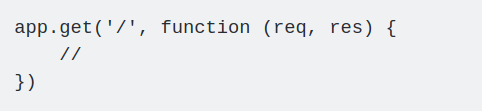
\includegraphics[width = 10cm]{image/res-req.png}
        \caption{Request \& Response}
        \label{fig:req_res}
    \end{figure}
    \begin{itemize}
        \item \textbf{Request} - Biểu diễn một HTTP request và có các thuộc tính cho các request như các chuỗi truy vấn, tham số, body, HTTP header và những phần khác.
        \item \textbf{Response} - Biểu diễn một HTTP response được ứng dụng Express gửi đi khi nó nhận về một HTTP request.
    \end{itemize}
    \item \textbf{Express route}\\
    Route là một thành phần cực kỳ quan trọng của một website, nó giúp website biết được người dùng truy cập đến nơi nào của trang web, từ đó phản hồi lại một cách thích hợp. Trong ExpressJs, route được tích hợp sẵn và dễ dàng sử dụng.
    \begin{enumerate}
        \item \textbf{Route methods}
        \begin{itemize}
            \item Có 4 phương thức \textbf{GET, POST, PUT, DELETE}
            \item Ví dụ về cách sử dụng: app.get('/', (req, res) => res.send('Hello World!'));
        \end{itemize}
        \item \textbf{Route parameters}
        \begin{figure}[H]
        \centering
        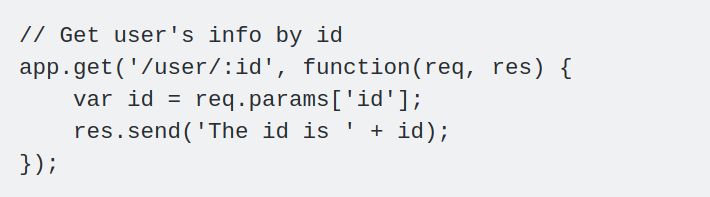
\includegraphics[width = 10cm]{image/route-parameter.png}
        \caption{Ví dụ về Route Parameter}
        \label{fig:route_parameter}
    \end{figure}
    \end{enumerate}
\end{enumerate}

\newpage
\section{Cơ sở dữ liệu}
\textbf{Khái niệm:}

Cơ sở dữ liệu (Database) là một tập hợp các dữ liệu có tổ chức, thường được lưu trữ và truy cập điện tử từ hệ thống máy tính. Khi cơ sở dữ liệu phức tạp hơn, chúng thường được phát triển bằng cách sử dụng các kỹ thuật thiết kế và mô hình hóa chính thức.\\

\textbf{Phân loại:}
\begin{itemize}
    \item Cơ sở dữ liệu quan hệ (SQL)
    \item Cơ sở dữ liệu phi quan hệ (NoSQL)
\end{itemize}

\textbf{So sánh cơ sở dữ liệu quan hệ và phi quan hệ:}
\begin{table}[H]
	    \centering
	    \begin{tabular}{|p{3cm}|p{6cm}|p{6cm}|}
	    \hline
	    &Cơ sở dữ liệu quan hệ&Cơ sở dữ liệu phi quan hệ\\
	    \hline
	    Ngôn ngữ truy vấn&Ngữ truy vấn có cấu trúc&Sử dụng ngôn ngữ truy vấn không cấu trúc\\
	    \hline
	    Cấu trúc&Biểu thị dữ liệu dưới dạng bảng, hàng và cột&Biểu thị dữ liệu dưới dạng biểu đồ, các cặp khóa-giá trị và nhiều hơn thế.\\
	    \hline
	    Khả năng mở rộng&Mở rộng thêm chiều dọc&Mở rộng theo chiều ngang\\
	    \hline
	    Chi phí&Chi phí xây dựng và bảo trì cao&Khoảng 10\% so với cơ sở dữ liệu quan hệ\\
	    \hline
	    \end{tabular}
	    \caption{So sánh cơ sở dữ liệu quan hệ và phi quan hệ}
\end{table}
\subsection{Ngôn ngữ truy vấn có cấu trúc (SQL)}
\subsubsection{SQL là gì?}
SQL là loại ngôn ngữ máy tính, giúp cho thao tác lưu trữ và truy xuất dữ liệu được lưu trữ trong một cơ sở dữ liệu quan hệ. SQL là viết tắt của Structured Query Language là ngôn ngữ truy vấn có cấu trúc.

Tất cả RDBMS (hệ thống quản lý cơ sở dữ liệu quan hệ) như đều sử dụng SQL như là ngôn ngữ cơ sở dữ liệu chuẩn.

SQL là một ngôn ngữ được tiêu chuẩn hóa bởi ANSI (American National Standards Institute) – Viện tiêu chuẩn quốc gia Hoa Kỳ. Đây cũng đồng thời là ngôn ngữ được sử dụng phổ biến trong các hệ thống quản lý cơ sở dữ liệu quan hệ và hỗ trợ sử dụng trong các công ty lớn về công nghệ.
\subsubsection{Tại sao phải sử dụng SQL?}
SQL thường được các RDBMS sử dụng để tương tác với cơ sở dữ liệu thông qua các thao tác sau:
\begin{itemize}
    \item Tạo cơ sở dữ liệu, bảng và view mới.
    \item Để chèn các bản ghi vào trong một cơ sở dữ liệu.
    \item Để xóa các bản ghi từ một cơ sở dữ liệu.
    \item Để lấy dữ liệu từ một cơ sở dữ liệu.
\end{itemize}
\subsubsection{Chức năng}
Một trong những lý do khiến cho SQL được sử dụng phổ biến, chính là nó đã cho phép người dùng thực hiện đa dạng các chức năng sau:
\begin{itemize}
    \item Cho phép người dùng truy cập dữ liệu trong các hệ thống quản lý cơ sở dữ liệu quan hệ.
    \item Cho phép người dùng mô tả dữ liệu.
    \item Cho phép người dùng xác định dữ liệu trong cơ sở dữ liệu và thao tác dữ liệu đó.
    \item Cho phép nhúng trong các ngôn ngữ khác sử dụng mô-đun SQL, thư viện và trình biên dịch trước.
    \item Cho phép người dùng tạo và thả các cơ sở dữ liệu và bảng.
    \item Cho phép người dùng tạo chế độ view, thủ tục lưu trữ, chức năng trong cơ sở dữ liệu.
    \item Cho phép người dùng thiết lập quyền trên các bảng, thủ tục và view.
\end{itemize}
\subsubsection{Ưu điểm}
\begin{itemize}
    \item Dữ liệu có ở mọi nơi: Dữ liệu xuất hiện ở mọi nơi trên màn hình từ laptop đến điện thoại của bạn. Việc học tập và tìm hiểu SQL sẽ giúp bạn biết được cách thức hoạt động của những dữ liệu này.
    \item Thêm, sửa, đọc và xóa dữ liệu dễ dàng: với SQL, các thao tác xử lý dữ liệu trở nên dễ dàng hơn bao giờ hết. Bạn chỉ cần thực hiện một số thao tác với dữ liệu đơn giản trên SQL thay vì phải dùng nhiều câu lệnh phức tạp trên các loại ngôn ngữ khác.
    \item SQL giúp công việc lập trình dễ dàng hơn: bạn có thể lưu nhiều dữ liệu cho nhiều ứng dụng khác nhau trên cũng một cơ sở dữ liệu và việc truy cập các cơ sở dữ liệu này trở lên đơn giản hơn nhờ một cách thức giống nhau.
    \item Được sử dụng và hỗ trợ bởi nhiều công ty lớn: tất cả các công ty lớn về công nghệ trên thế giới hiện nay như Microsoft, IBM, Oracle… đều hỗ trợ việc phát triển ngôn ngữ SQL.
    \item Lịch sử hơn 40 năm: với lịch sử phát triển hơn 40 năm từ 1970, SQL vẫn tồn tại và trụ vững đến ngày nay. Điều này cho thấy vị trí của SQL hiện tại rất khó bị thay thế bởi bất kỳ một ngôn ngữ máy tính nào khác.
\end{itemize}
\subsection{Hệ cơ sở dữ liệu quan hệ (RDBMS)}
\textbf{Khái niệm:}

RDBMS - Relational Database Management System - là hệ cơ sở dữ liệu quan hệ. Tất cả các hệ thống quản trị cơ sở dữ liệu hiện đại như SQL, MySQL, MS SQL Server, Oracle, ... đều dựa trên RDBMS.

Hệ thống quản lý cơ sở dữ liệu quan hệ (RDBMS) là một hệ thống quản lý cơ sở dữ liệu (DBMS) dựa trên mô hình quan hệ được giới thiệu bởi EF Codd.\\

\textbf{Bảng (Table):}

RDBMS sử dụng các bảng để lưu trữ dữ liệu. Mỗi bảng là một tập hợp các dữ liệu có liên quan đến nhau và có nhiều hàng và cột để lưu dữ liệu. Bảng là hình thức lưu trữ phổ biến và đơn giản nhất trong môt cơ sở dữ liệu quan hệ. Ví dụ về bảng một nhóm môn học trong bảng MONHOC sau đây:\\
\begin{table}[H]
    \centering
    \begin{tabular}{|l|l|l|}
    \hline
         \textbf{ID}&\textbf{TEN\_MON\_HOC}&\textbf{SO\_TIN\_CHI}\\
         \hline
         1&Giải tích 1&4\\
		\hline
		2&Vật lý&3\\
		\hline			
		3&Kỹ thuật lập trình&4\\
		\hline
    \end{tabular}
    \caption{Ví dụ về bảng dữ liệu}
\end{table}

\textbf{Trường (Field):}
	
	Mỗi bảng được chia thành các thực thể nhỏ gọi là các trường, chứa các thông tin cụ thể về mỗi bản ghi trong bảng. Các trường trong bảng MONHOC bao gồm: ID, TEN\_MON\_HOC, SO\_TIN\_CHI.\\
	\begin{table}[H]
	    \centering
	    \begin{tabular}{|l|}
	        \hline
	        \textbf{TEN\_MON\_HOC}\\
	        \hline
	        Giải tích 1\\
	        \hline
	        Vật lý\\
	        \hline
	        Kỹ thuật lập trình\\
	        \hline
	    \end{tabular}
	    \caption{Ví dụ một trường trong bảng dữ liệu}
	\end{table}
	
\textbf{Hàng hoặc bản ghi (Record):}
	
Một hàng của bảng được gọi là bản ghi , nó chứa thông tin của một đối tượng trong bảng. Ví dụ ở bảng MONHOC có 3 bản ghi. Sau đây là một bản ghi trong bảng:\\
\begin{table}[H]
    \centering
    \begin{tabular}{|r|r|r|}
        \hline
		1&Giải tích 1&4\\
		\hline
    \end{tabular}
    \caption{Ví dụ về một bản ghi}
\end{table}
\newpage
\textbf{Ràng buộc (Constraint):}

Ràng buộc là các quy tắc cho các cột dữ liệu trong bảng. Chúng được sử dụng để giới hạn loại dữ liệu có thể insert vào một bảng. Điều này đảm bảo tính chính xác và độ tin cậy của dữ liệu trong cơ sở dữ liệu.\\
Constraint có thể là cấp độ cột hoặc cấp độ bảng. Các ràng buộc cấp độ cột chỉ được áp dụng cho một
cột trong khi các ràng buộc mức bảng được áp dụng cho toàn bộ bảng.\\
Sau đây là một số ràng buộc phổ biến nhất được sử dụng trong SQL :\\
\begin{table}[H]
    \centering
    \begin{tabular}{|l|l|}
        \hline
         NOT NULL&Đảm bảo rằng một field không có giá trị NULL  \\
         \hline
         DEFAULT&Cung cấp giá trị mặc định của một field khi không được xác định\\
         \hline
         UNIQUE&Đảm bảo giá trị trong một field là khác nhau\\
         \hline
         PRIMARY Key&Mỗi record là duy nhất trong một bảng cơ sở dữ liệu\\
         \hline
         FOREIGN Key&Mỗi record là duy nhất trong trong bất kỳ bảng cơ sở dữ liệu khác\\
         \hline
         CHECK&Đảm bảo rằng tất cả các giá trị trong một cột thỏa mãm một số điều kiện\\
         \hline
         INDEX&Dùng để tạo và lấy dữ liệu một cách nhanh chóng\\
         \hline
    \end{tabular}
    \caption{Một số ràng buộc phổ biến trong SQL}
\end{table}
\subsection{Hệ quản trị cơ sở dữ liệu}

Hệ quản trị cơ sở dữ liệu (Database Management System - DBMS) là hệ thống kiểm soát việc lưu trữ, tổ chức và truy xuất dữ liệu.

Mỗi DBMS đều có thành phần gọi là Query Language (Ngôn ngữ truy vấn), các ứng dụng muốn truy cập dữ liệu đều phải nhờ vào thành phần này.

Các hệ quản trị cơ sở dữ liệu quan hệ phổ biến nhất hiện nay:
\subsubsection{Oracle Database}
\begin{center}
  \captionsetup{type=figure}
  
\includegraphics[scale=0.4]{image/oracle.jpg}
  \captionof{figure}{Oracle Database}
\end{center}


\textbf{Oracle là gì?}


Oracle Database hay còn gọi là Oracle RDBMS hoặc đơn giản là Oracle là 1 hệ quản trị cơ sở dữ liệu quan hệ, được phát triển và phân phối bởi tập đoàn Oracle

Cơ sở dữ liệu Oracle là cơ sở dữ liệu đầu tiên được thiết kế cho điện toán lưới doanh nghiệp, cách linh hoạt và tiết kiệm chi phí nhất để quản lý thông tin và ứng dụng. Điện toán lưới doanh nghiệp tạo ra các nhóm lớn máy chủ và lưu trữ mô-đun theo tiêu chuẩn công nghiệp. Với kiến trúc này, mỗi hệ thống mới có thể được cung cấp nhanh chóng từ nhóm các thành phần. Không cần khối lượng công việc cao nhất, bởi vì công suất có thể dễ dàng được thêm hoặc phân bổ lại từ các nguồn tài nguyên khi cần thiết.\\

\textbf{Đặc điểm của Oracle}
\begin{itemize}
    \item Quản lý được hệ thống dữ liệu lớn
    \item Hỗ trợ nhiều công cụ để quản trị cũng như nhập, xuất dữ liệu dễ dàng
    \item Có thể hoạt động trên nhiều hệ điều hành khác nhau như Windows, Linux, Mac OS, Unix,...
    \item Truy cập đồng thời
    \item Hỗ trợ cơ chế khóa
    \item Thực thi song song
    \item Tính khả chuyển
\end{itemize}

\textbf{Thế mạnh của Oracle:}
\begin{itemize}
    \item \textit{Hệ thống quản lý và kiểm soát tập trung:} Điều này cho phép dữ liệu được kiểm soát hoàn toàn từ một trao đổi dạng bảng vì nó chịu trách nhiệm gán, thêm, xóa các bản ghi và sửa đổi chúng.
    \item \textit{Tiêu chuẩn hóa:} Cho phép tiêu chuẩn hóa giữa các triển khai SQL khác nhau.
    \item \textit{Nhóm các giao dịch:} Nó cho phép nhóm một số giao dịch và chia từng hoạt động thành các phân khúc và do đó đạt được hiệu suất tốt hơn trong thời gian ngắn hơn có thể.
    \item \textit{Phương thức hiệu suất:} Áp dụng các phương pháp để cải thiện cơ sở dữ liệu thông qua ứng dụng Cluster.
\end{itemize}
\subsubsection{MySQL}
\begin{center}
  \captionsetup{type=figure}
    
\includegraphics[scale=0.5]{image/mysql.jpg}
  \captionof{figure}{MySQL}
\end{center}

MySQL là một hệ quản trị cơ sở dữ liệu quan hệ mã nguồn mở, được phát triển, phân phối và hỗ trợ bởi tập đoàn Oracle.\\

\textbf{MySQL hoạt động như thế nào?}

MySQL hoạt động dưới hình thức client-server:
\begin{itemize}
    \item MySQL tạo một cơ sở dữ liệu để lưu trữ và thao tác dữ liệu, xác định mối quan hệ của từng bảng.
    \item Khách hàng có thể thực hiện các yêu cầu bằng cách nhập các câu lệnh SQL cụ thể trên MySQL.
    \item Ứng dụng máy chủ sẽ phản hồi với thông tin được yêu cầu và nó sẽ xuất hiện ở phía máy khách.
\end{itemize}


\textbf{Đặc điểm và thế mạnh:}
\begin{itemize}
    \item \textit{Tính nội bộ và linh động:}
    \begin{itemize}
    \item Viết bằng C và C++
    \item Đã thử nghiệm với một loạt các trình biên dịch khác nhau
    \item Hoạt động trên nhiều nền tảng khác nhau
    \item Sử dụng thiết kế máy chủ nhiều lớp với các mo-đun độc lập
    \item Được thiết kế để đa luồng hoàn toàn bằng cách sử dụng các luồng nhân, để dễ dàng sử dụng nhiều CPU nếu chúng có sẵn
    \item Triển khai các bảng băm trong bộ nhớ, được sử dụng làm bảng tạm thời.
    \item Triển khai các hàm SQL bằng cách sử dụng thư viện lớp được tối ưu hóa cao nhất phải nhanh nhất có thể
    \end{itemize}
    \item \textit{Bảo mật}
    \begin{itemize}
        \item Một hệ thống đặc quyền và mật khẩu rất linh hoạt và an toàn, và cho phép xác minh dựa trên máy chủ
        \item Bảo mật mật khẩu bằng cách mã hóa tất cả lưu lượng mật khẩu khi bạn kết nối với máy chủ.
    \end{itemize}
    \item \textit{Khả năng mở rộng và giới hạn:}
    \begin{itemize}
        \item Hỗ trợ cơ sở dữ liệu lớn
        \item Hỗ trợ lên đến 64 chỉ mục cho mỗi bảng
    \end{itemize}
    \item \textit{Ổn định, có tốc độ cao và dễ sử dụng}
    \item \textit{Đa tính năng:} Hỗ trợ rất nhiều chức năng SQL
\end{itemize}
\subsubsection{SQL Server}
\begin{center}
  \captionsetup{type=figure}
    
\includegraphics[scale=0.3]{image/sql-server.png}
  \captionof{figure}{SQL Server}
\end{center}
\textbf{SQL Server là gì?}

SQL Server là một RDBMS được phát triển bởi tập đoàn Microsoft. Tương tự như phần mềm RDBMS khác, SQL Server được xây dựng dựa trên SQL, một ngôn ngữ lập trình tiêu chuẩn để tương tác với các cơ sở dữ liệu quan hệ. Máy chủ SQL được liên kết với Transact-SQL hoặc T-SQL, triển khai SQL Microsoft Microsoft bổ sung một tập hợp các cấu trúc lập trình độc quyền. SQL Server hoạt động độc quyền trên môi trường Windows trong hơn 20 năm. Năm 2016, Microsoft đã cung cấp nó trên Linux. SQL Server 2017 thường có sẵn vào tháng 10 năm 2016 chạy trên cả Windows và Linux.\\
\newline
\textbf{SQL Server hoạt động như thế nào?}
\begin{itemize}
    \item Giống như các công nghệ RDBMS khác, SQL Server chủ yếu được xây dựng xung quanh cấu trúc bảng dựa trên hàng để kết nối các thành phần dữ liệu liên quan trong các bảng khác nhau với nhau, tránh việc lưu trữ dữ liệu ở nhiều nơi trong cơ sở dữ liệu. Mô hình quan hệ cũng cung cấp tính toàn vẹn tham chiếu và các ràng buộc toàn vẹn khác để duy trì độ chính xác của dữ liệu. Các kiểm tra này là một phần của việc tuân thủ rộng hơn các nguyên tắc về tính nguyên tử, tính nhất quán, độ cô lập và độ bền, được gọi chung là các thuộc tính ACID và được thiết kế để đảm bảo rằng các giao dịch cơ sở dữ liệu được xử lý một cách đáng tin cậy.
    \item Thành phần cốt lõi của SQL Server là SQL Server Database Engine, điều khiển lưu trữ, xử lý và bảo mật dữ liệu. Nó bao gồm một công cụ quan hệ xử lý các lệnh và truy vấn và một công cụ lưu trữ quản lý các tệp cơ sở dữ liệu, bảng, trang, chỉ mục, bộ đệm dữ liệu và giao dịch. Các thủ tục lưu trữ, kích hoạt, khung nhìn và các đối tượng cơ sở dữ liệu khác cũng được tạo bởi Cơ sở dữ liệu.
    \item Bên dưới cơ sở dữ liệu là Hệ điều hành Máy chủ SQL hoặc SQLOS. SQLOS xử lý các chức năng cấp thấp hơn, chẳng hạn như quản lý bộ nhớ và I/O, lập lịch công việc và khóa dữ liệu để tránh các cập nhật xung đột. Một lớp giao diện mạng nằm phía trên Cơ sở dữ liệu và sử dụng giao thức Luồng dữ liệu dạng bảng của Microsoft để tạo điều kiện cho các tương tác yêu cầu và phản hồi với các máy chủ cơ sở dữ liệu. Và ở cấp độ người dùng, các DBA và nhà phát triển SQL Server viết các câu lệnh T-SQL để xây dựng và sửa đổi cấu trúc cơ sở dữ liệu, thao tác dữ liệu, thực hiện bảo vệ an ninh và sao lưu cơ sở dữ liệu, trong số các tác vụ khác
\end{itemize}
\textbf{Thế mạnh:}
\begin{itemize}
    \item Cho phép nhiều người dùng chung một cơ sở dữ liệu
    \item Duy trì lưu trữ bền vững
    \item Khả năng mở rộng
    \item Tính bảo mật cao
    \item Độ tin cậy, bảo vệ dữ liệu
    \item Hỗ trợ phân tích dữ liệu
    \item Kết hợp tốt với các sản phẩm của Microsoft
    \item Có thể sao lưu, khôi phục dữ liệu một cách dễ dàng
\end{itemize}

\subsubsection{PostgreSQL}
\begin{center}
  \captionsetup{type=figure}
    
\includegraphics[scale=0.5]{image/postgre-sql.jpg}
  \captionof{figure}{PostgreSQL}
\end{center}

PostgreSQL là một RDBMS mở nguồn mở được xây dựng trên mã nguồn ban đầu của đại học Berkeley.

\textit{Đặc điểm và thế mạnh:}
\begin{itemize}
    \item Truy xuất dữ liệu tốc độ nhanh
    \item Sử dụng câu truy vấn phức tạp
    \item Sử dụng khóa ngoại
    \item Có thủ tục
    \item Đảm bảo tính toàn vẹn của các giao tác
\end{itemize}

\subsection{Hệ cơ sở dữ liệu phi quan hệ (Non-RDBMS)}
Hệ cơ sở dữ liệu phi quan hệ là cơ sở dữ liệu không sử dụng mô hình bảng gồm các cột và hàng như nhiều hệ cơ sở dữ liệu truyền thống. Thay vào đó, Non-RDBMS sử dụng mô hình lưu trữ được tối ưu hóa cho các yêu cầu cụ thể của loại dữ liệu được lưu trữ. Cơ sở dữ liệu phi quan hệ (Non-relational database) phổ biến nhất được gọi là NoSQL.\\
Các Non-RDBMS phổ biến:
\subsubsection{MongoDB}
\begin{center}
  \captionsetup{type=figure}
    
\includegraphics[width=10cm]{image/mongo.png}
  \captionof{figure}{MongoDB}
\end{center}

MongoDB (chữ mongo được lấy từ từ humongous trong tiếng Anh), là một NoSQL database. Khác với MySQL hay các loại SQL databse khác chạy theo mô hình database – table – row với số dòng – cột nhất định, schema phức tạp, và phải sử dụng nhiều Join khi query. MongoDB chạy theo mô hình database – collection – document, thay thế mô hình cơ sở dữ liệu dùng table truyền thống bằng các document với định dạng JSON với cấu trúc linh hoạt hơn (MongoDB gọi là BSON).

Các thuật ngữ thường sử dụng trong MongoDB:
\begin{itemize}
    \item \textbf{\_id:} Là trường bắt buộc có trong mỗi document. Trường \_id đại diện cho một giá trị duy nhất trong document MongoDB. Trường \_id cũng có thể được hiểu là khóa chính trong document. Nếu bạn thêm mới một document thì MongoDB sẽ tự động sinh ra một \_id.
    \item \textbf{Collection:} Collection là một nhóm các Document trong MongoDB. Nó tương đương như một bảng trong RDBMS. Do đó, một Collection tồn tại bên trong một cơ sở dữ liệu duy nhất. Các Collection không có ràng buộc Relationship như các hệ quản trị cơ sở dữ liệu khác nên việc truy xuất rất nhanh, chính vì thế mỗi collection có thể chứa nhiều thể loại khác nhau không giống như table trong hệ quản trị mysql là các field cố định. Các Document bên trong một Collection có thể có nhiều trường khác nhau. Đặc biệt, tất cả các Document trong một Collection là tương tự nhau hoặc với cùng mục đích liên quan.
    \item \textbf{Cursor:} Đây là một con trỏ đến tập kết quả của một truy vấn. Máy khách có thể lặp qua một con trỏ để lấy kết quả.
    \item \textbf{Database:} Chính là tập chứa các collection trong MongoDB. Mỗi database sẽ có một tập file riêng của mình trên file system của hệ thống. Một MongoDB server thường chứa nhiều database trên đó.
    \item \textbf{Document:} Là một tập dữ liệu theo dạng key-value, mỗi key sẽ tương ứng với một value. Các document khá linh hoạt về schema, như đã nói ở trên, các document trong cùng một collection không nhất thiết phải có các field hoặc cấu trúc giống nhau. Data trong cùng một field cũng có thể có nhiều kiểu dữ liệu khác nhau.
    \item \textbf{Field:} Là một cặp name-value trong một document.
    \item \textbf{JSON:} Các document của MongoDB sử dụng format JSON (JavaScript Object Notation), đây là một chuẩn lưu trữ, trao đổi dữ liệu đơn giản và gọn nhẹ. Với ưu điểm dễ đọc, dễ hiểu, đa phần các ngôn ngữ lập trình phổ biến hiện nay đều hỗ trợ JSON như: C, C++, Java, JavaScript, Perl, Python,….Dữ liêu trong JSON được lưu trữ dưới dạng key/value. Một key sẽ tương ứng với 1 value. Value ở đây có thể là một mảng, một chuỗi, một số int, double, mảng hoặc object… .
    
    
\end{itemize}

\textit{Thế mạnh:}
\begin{itemize}
    \item Ít schema hơn
    \item Cấu trúc của một đối tượng rõ ràng
    \item Không có các phép join phức tạp
    \item Khả năng mở rộng cực lớn: Việc mở rộng dữ liệu mà không cần phải quan tâm đến các vấn đề như khóa ngoại, khóa chính, kiểm tra ràng buộc,...
    \item Sử dụng bộ nhớ trong để lưu giữ cửa sổ làm việc cho phép truy cập dữ liệu nhanh hơn. Việc cập nhật được thực hiện nhanh gọn nhờ update tại chỗ (in-place).
    \item Hỗ trợ nhiều công cụ lưu trữ
\end{itemize}

\textit{Các thao tác cơ bản trong MongoDB}
\begin{description}
\item 1.Create:\\
Tạo hoặc thêm một document mới vào collection, nếu collection đó chưa tồn tại thì sẽ tạo mới collection

MongoDB cung cấp hai phương thức để chèn thêm một document:
\begin{itemize}
    \item db.collection.insertOne(): chèn một tài liệu mới vào một collection. Nếu document không có trường \_id , MongoDB sẽ tự động thêm trường \_id với value kiểu ObjectId.
\begin{verbatim}
db.inventory.insertOne(
    { item: "canvas", qty: 100, tags: ["cotton"], size:{ h: 28, w: 35.5}}
)
\end{verbatim}
    \item db.collection.insertMany(): chèn nhiều document vào một collection, truyền vào phương thức là mảng các document
\begin{verbatim}
db.inventory.insertMany([
    {item: "journal", qty: 25, tags: ["blank", "red"], size:{h: 14, w: 21}},
    {item: "mat", qty: 85, tags: ["gray"], size:{h: 27.9, w: 35.5}},
    {item: "mouse", qty: 25, tags: ["gel", "blue"], size:{h: 19, w: 22.85}}
])
\end{verbatim}
\end{itemize}
\item 2.Read\\
Truy xuất document từ một collection. Để lấy ra toàn bộ document của ta sử dụng phương thức find
\begin{verbatim}
        db.inventory.find()
\end{verbatim}
\item 3. Update\\
Thao tác update cho phép chình sửa document trong collection
\begin{itemize}
    \item Cập nhật một document với db.collection.updateOne():
    \begin{verbatim}
        db.inventory.updateOne(
           { item: "paper" },
           {
             $set: { "size.uom": "cm", status: "P" }
           }
        )
    \end{verbatim}
    \item Cập nhật nhiều Document với db.collection.updateMany():
    \begin{verbatim}
        db.inventory.updateMany(
           { "qty": { $lt: 50 } },
           {
             $set: { "size.uom": "in", status: "P" },
             $currentDate: { lastModified: true }
           }
        )
    \end{verbatim}
    \item Thay thế một document: Để thay thế toàn bộ nội dung của một document (ngoại trừ trường \_id), truyền vào toàn bộ document mới là một tham số thứ hai của hàm. Ví dụ dưới đây thay thế document đầu tiên từ collection inventory mà có item bằng "paper"
\begin{verbatim}
db.inventory.replaceOne(
    {item:"paper"},
    {item: "paper",instock:[{warehouse:"A",qty:60},{warehouse:"B",qty:40}]}
)
\end{verbatim}
\end{itemize}
\item 4. Delete\\
\begin{itemize}
    \item Xóa một document thỏa mãn điều kiện: Để xóa chỉ một document phù hợp với điều kiện (trường hợp có nhiều document thỏa mãn thì sẽ xóa document đầu tiên), sử dụng db.collection.deleteOne(filter)
    \item Xóa tất cả document thỏa mãn điều kiện: sử dụng db.collection.deleteMany(filter)

\end{itemize}
\end{description}
\subsection{So sánh Relational Database và Non-Relational Database}
\begin{table}[H]
	    \centering
	    \begin{tabular}{|p{3cm}|p{6cm}|p{6cm}|}
	        \hline
	        &\textbf{Relational}&\textbf{Non-Relational}\\
	        \hline
	        Ngôn ngữ truy vấn&Ngôn ngữ truy vấn có cấu trúc &Truy vấn đối tượng: trực quan, chuyển một tài liệu để giải thích những gì bạn đang truy vấn\\
	        \hline
	        Kiểu dữ liệu&Lưu các kiểu dữ liệu được quy định&Có thể lưu bất kỳ loại dữ liệu nào\\
	        \hline
	        Khả năng mở rộng&Mở rộng thêm chiều dọc&Mở rộng theo chiều ngang\\
	        \hline
	        Hiển thị dữ liệu&Dưới dạng bảng và hàng&Dưới dạng JSON\\
	        \hline
	        Chi phí&Chi phí xây dựng và bảo trì cao&Khoảng 10\% so với Relational\\
	        \hline
	    \end{tabular}
	    \caption{So sánh cơ sở dữ liệu quan hệ và cơ sở dữ liệu phi quan hệ}
	\end{table}
\subsection{Kết luận và lựa chọn}

Dựa vào các đối tượng mà hệ thống hướng tới, hệ thống cần lưu trữ lượng dữ liệu lớn, đáp ứng trong thời gian nhanh. Nhóm quyết định lựa chọn sửa dụng \textbf{MongoDB}.\\
\begin{itemize}
    \item Dữ liệu trong MongoDB không có sự ràng buộc lẫn nhau như trong RDBMS, khi insert, xóa hay update nó không cần phải mất thời gian kiểm tra xem có thỏa mãn các bảng liên quan như trong RDBMS.
    \item Dữ liệu trong MongoDB được đánh chỉ mục (đánh index) nên khi truy vấn nó sẽ tìm rất nhanh
    \item Khi thực hiện insert, find… MongoDB sẽ khóa các thao tác khác lại, ví dụ khi nó thực hiện find(), trong quá trình find mà có thêm thao tác insert, update thì nó sẽ dừng hết lại để chờ find() xong đã.

\end{itemize}


% \textbf{Node-oracledb:}
% Thay vì phải sử dụng các câu query thuần để kết nối, truy cập, định nghĩa cấu trúc
% database, chúng ta có thể sử dụng các hàm do Node-oracledb cung cấp để làm những việc này
% một cách dễ dàng, ngắn gọn, nhanh chóng hơn.
% \begin{figure}[ht]
%     \centering
%     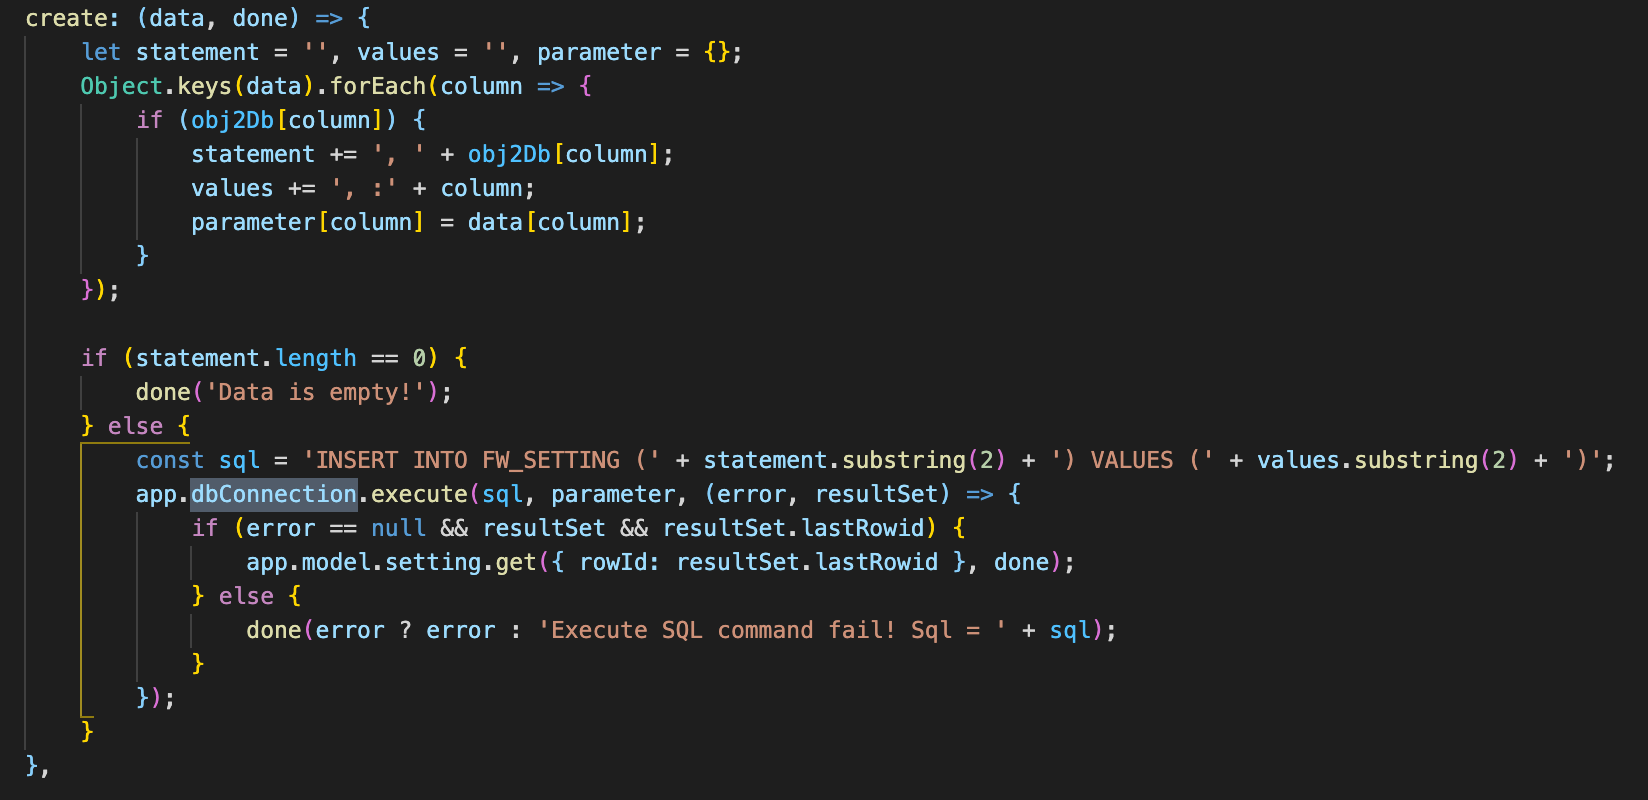
\includegraphics[width=10cm]{image/nodeoracledb.png}
%     \caption{Ví dụ về việc sử dụng node-oracledb}
% \end{figure}


% Việc truy vấn dữ liệu cũng dễ dàng, thuận tiện hơn khi Node-oracledb hỗ trợ các hàm truy
% vấn.
\section{REST API}
\subsection{Giới thiệu REST API:}
REST (REpresentational State Transfer) là một tiêu chuẩn thiết kế API (API architectural style) cho các ứng dụng. REST được giới thiệu lần đầu tiên bởi Roy Fielding vào năm 2000 trong luận án nổi tiếng của ông ``Architectural Styles and
the Design of Network-based Software Architecture'' đại học California.

Mặc dù REST có thể sử dụng trên hầu hết mọi giao thức ứng dụng phần mềm, nhưng REST thường biết đến rộng rãi trong các giao thức của ứng dụng Web vì tận dụng được những lợi thế của HTTP, giúp nhà phát triển không cần cài đặt thêm phần mềm hoặc thư viện bổ sung để sử dụng REST API.

\subsection{Một số đặc điểm cơ bản của REST:}
\begin{itemize}
    \item \textbf{Uniform interface:} Các API được thiết kế một cách nhất quán theo các nguyên tắc chung. Ví dụ luôn luôn sử dụng danh từ số nhiều thay vì khi số nhiều, khi số ít, sử dụng dấu gạch ngang để phân tách giữa các từ. Tài nguyên của hệ thống phải tuân theo các quy tắt đặt tên, định dạng dữ liệu (JSON hay XML), được truy cập thông qua một cách tiếp cận phổ biến như HTTP GET và được sửa đổi thông qua các phương thức tương tự.
    \item \textbf{Client-Server:} Client và Server không cần phụ thuộc vào nhau, có thể phát triển độc lập, thậm chí sửa đổi, thay thế miễn sao interface giao tiếp giữa chúng vẫn được giữ nguyên.
    \item \textbf{Stateless}: Server không lưu trữ bất kì thông tin gì về yêu cầu của client, nó sẽ coi mọi yêu cầu là mới. Không section, không history. Vì vậy, mỗi yêu cầu từ client tới server phải chứa tất cả các thông tin cần thiết để  server hiểu được yêu cầu đó.
    \item \textbf{Code on demand:} Sử dụng HTTP status code khi có thể
\end{itemize}


\subsection{Những lợi ích khi sử dụng REST API:}

- Nhờ tính độc lập giữa client và server, nhà phát triển có thể dễ dàng phát triển, sửa đổi thậm chí thay thế client và server miễn sao vẫn giữ nguyên interface giao tiếp giữa chúng.

- API REST luôn độc lập với loại nền tảng hoặc ngôn ngữ: API REST luôn thích nghi với loại cú pháp hoặc nền tảng đang được sử dụng, điều này mang lại sự tự do đáng kể khi thay đổi hoặc kiểm tra môi trường mới trong quá trình phát triển. Với API REST, bạn có thể có máy chủ với các ngôn ngữ như PHP, Java, Python hoặc Node.js.

- Tính nhất quán: Các API được thiết kế một cách nhất quán giúp cho việc phát triển, bảo trì đơn giản hơn, đặc biệt phù hợp với các hệ thống có nhiều module.

%%%%%%%%%%%%%%%%%%%%%%%%%%%%%%%%%%%%%%%%%%%%%%%%%%%%%%%%
\chapter{\textbf{PHÂN TÍCH VÀ THIẾT KẾ HỆ THỐNG}}
%%%%%%%%%%%%%%%%%%%%%%%%%%%%%%%%%%%%%%%%%%%%%%%%%%%%%%%%%%%%%%%%%
\section{Phân tích yêu cầu hệ thống}
Hệ thống có thể được sử dụng bởi số lượng lớn người dùng. Mỗi ngừời dùng/quản lý sẽ có một tài khoản riêng cho mình. Mỗi tài khoản sẽ có một số lĩnh vực được cho phép sử dụng các chức năng khác nhau nằm trong quyền hạn của mình. Hệ thống website du lịch có thể được tóm gọn trong các chức năng như sau: 
\subsection{Quản trị viên}
Quản trị viên có toàn quyền sử dụng bất cứ chức năng nào của hệ thống như quản lý người dùng:
\begin{itemize}
    \item Hiển thị danh sách toàn bộ người dùng, bài viết, thông tin kế hoạch chuyến đi. 
    \item Quản lý thông tin người dùng: thông tin bao gồm các thông tin cá nhân và một số thông tin của người thân. Hệ thống cho phép chỉnh sửa và cập nhật khi thông tin có thay đổi.
    \item Hiển thị, thêm, xoá, sửa vai trò và quyền của người dùng.
    \item Hiện thị, thêm, xoá, sửa các bảng danh mục.
    \item Quản lý thông tin bài review.
    \item Quản lý thông tin chuyến đi.
    \item Quản lý thông tin cộng tác viên.
    \item Quản lý thông tin bình luận, đánh giá của bài review và chuyến đi.
\end{itemize}
\subsection{Cộng Tác Viên}
\begin{itemize}
    \item Cấu hình giá.
    \item Hiện thị, thêm, xoá, sửa sự kiện.
    \item Nếu không có quyền tạo sự kiện thì sự kiện được tự động tạo bản nháp và chờ người có quyền duyệt.
    
\end{itemize}
\subsection{Người dùng}
\begin{itemize}
    \item Quản lý thông tin cá nhân.
    \item Quản lý bài review.
    \item Quản lý thông tin chuyến đi.
    \item Quản lý thông tin bình luận của mình trong bài review.
        \subitem 
\end{itemize}
\subsection{Gửi thông báo bằng email}
Hệ thống gửi thông báo qua email khi có những hành động liên quan đến các sự kiện và thông tin chuyến đi:
\begin{itemize}
    \item Thông báo bài viết đã được phê duyệt.
    \item Khi một người dùng đăng ký tham chuyến đi. 
    \item Thông báo khi kế hoạch chuyến đi đã đủ người tham gia.
\end{itemize}
\section{Tổng quát kiến trúc hệ thống}
\indent 
    Hệ thống được xây dựng theo mô hình MVC kết hợp với REST API (RESTful). Ngoài ra để xử lý các tác vụ real time, nhóm sử dụng lớp Socket.io ở giữa tầng View và Controller.
Vận dụng kiến trúc REST API trong hệ thống:
Các API trong hệ thống Website du lịch Goz được thiết kế theo các nguyên tắc chung, nhất quán giữa các module.
\begin{itemize}
    \item API được đặt tên theo quy định chung, phù hợp với công dụng, quyền của API, thống nhất giữa các module.
    \begin{itemize}
        \item \textit{``/api/event/page/:pageNumber/:pageSize''}: API lấy tất cả dữ liệu của một bảng sự kiện. Ta có thể thấy các API có cấu trúc thống nhất với nhau với các bảng khác.
        \item \textit{``/api/draft-event/item/:eventId''}: API lấy dữ liệu của bảng sự kiện theo ID.
    \end{itemize}
    \item Sử dụng các phương thức HTTP (GET, POST, PUT, DELETE) để truy cập và xử lý dữ liệu.
    \begin{itemize}
        \item  \textit{GET /api/event/page/:pageNumber/:pageSize}: cách dùng API để lấy dữ liệu.
        \item  \textit{POST /api/event/default}: cách dùng API để thêm dữ liệu.
        \item  \textit{PUT /api/event/swap}: cách dùng API để sửa đổi dữ liệu.
        \item  \textit{DELETE /api/draft-event}: cách dùng API để xoá dữ liệu.
    \end{itemize}
    \item Dữ liệu được server trả về theo định dạng JSON.
    \item Server trả về các HTTP code phù hợp.
    \begin{itemize}
        \item  400 Invalid parameter: Trả về lỗi này khi client gửi yêu cầu sai cú pháp.
        \item  403 Can not access data: Trả về lỗi này khi client không có quyền truy cập dữ liệu.
        \item  404 Not found: Trả về lỗi này khi server không tìm thấy dữ liệu client yêu cầu.
    \end{itemize}
\end{itemize}

Nhận thấy mô hình MVC có nhiều ưu điểm và phù hợp với hệ thống (trình bày ở mục 2.1 Mô hình Model-View-Controller) nên nhóm đã sử dụng mô hình này trong thiết kế kiến trúc hệ thống.\\

Vận dụng mô hình MVC trong hệ thống Website du lịch Goz:
\begin{center}
  \captionsetup{type=figure}
  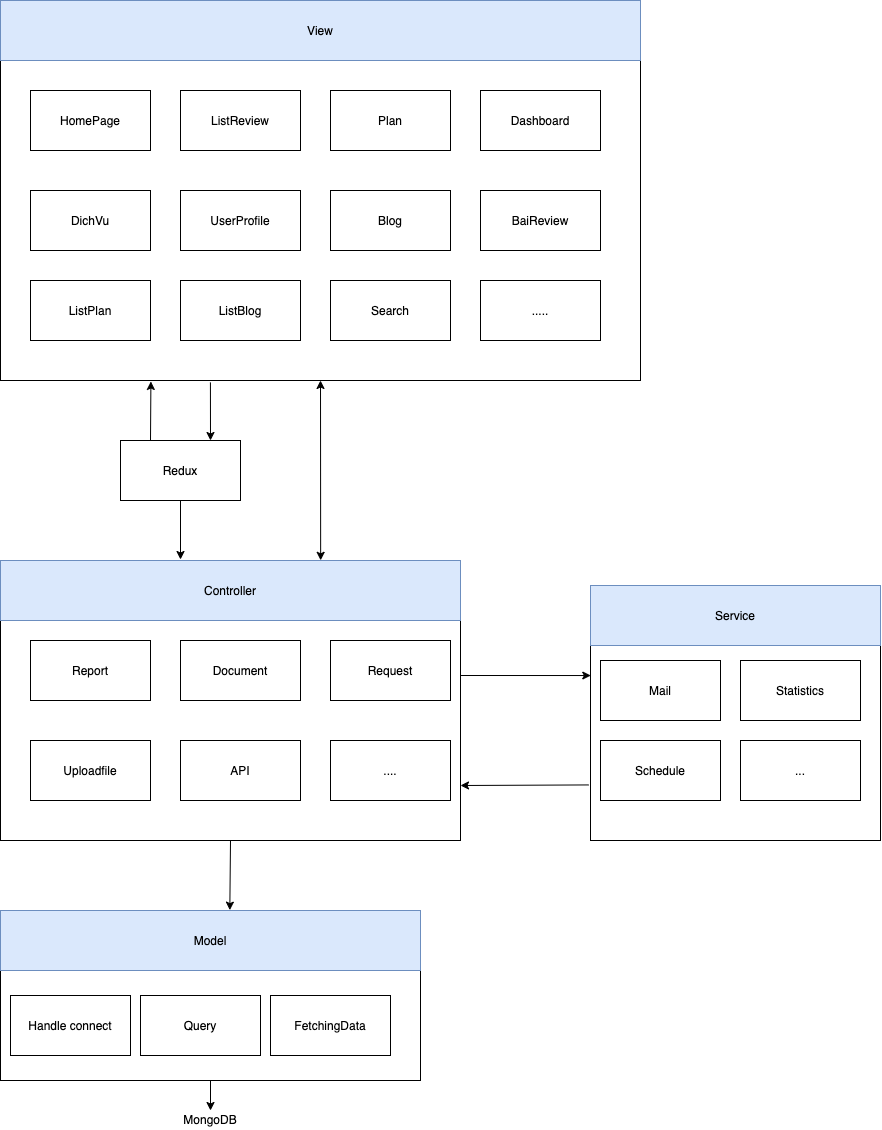
\includegraphics[width=15cm]{image/MVC11.png}
  \captionof{figure}{Kiến trúc tổng thể của hệ thống}
\end{center}

\section{Thiết kế đối tượng người dùng}
\subsection{Danh sách đối tượng người dùng}
Dựa vào những yêu cầu thực tế của hệ thống và những khảo sát thực tế đối với các cá nhân có nhu cầu sử dụng, xây dựng hệ thống Website du lịch Goz. Nhóm đưa ra các vai trò, người dùng chính trong hệ thống như sau:
\begin{table}[H]
    \centering
	\begin{tabular}{|p{1cm}|p{4cm}|p{10cm}|}
    \hline
    \textbf{STT}&\textbf{Người dùng}&\textbf{Đặc tả}\\
    \hline
    1&Khách&Là những người dùng chưa đăng nhập, bao gồm tất cả các đối tượng truy cập vào website như học sinh, sinh viên, phụ huynh, đơn vị, doanh nghiệp,...
    
    Khách có chức năng xem thông tin, tin tức, sự kiện, bài review của website, gửi email liên hệ,đăng kí và đăng nhập.\\
    \hline
	2&Người dùng ( thành viên đã đăng kí )& Người sử dụng có thể sử dụng tất cả các chức năng của trang web như tạo lịch trình chuyến đi cũng như đăng bài review, chia sẻ thông tin chuyến đi của mình với bạn bè. \\
	\hline
    3&Quản lí trang web& Người quản lí thông tin tất cả các tài khoản người dùng, duyệt bài review chuyến đi.\\
   
	\hline
\end{tabular}
\caption{Danh sách đối tượng người dùng của hệ thống}
\end{table}
\begin{center}
  \captionsetup{type=figure}
  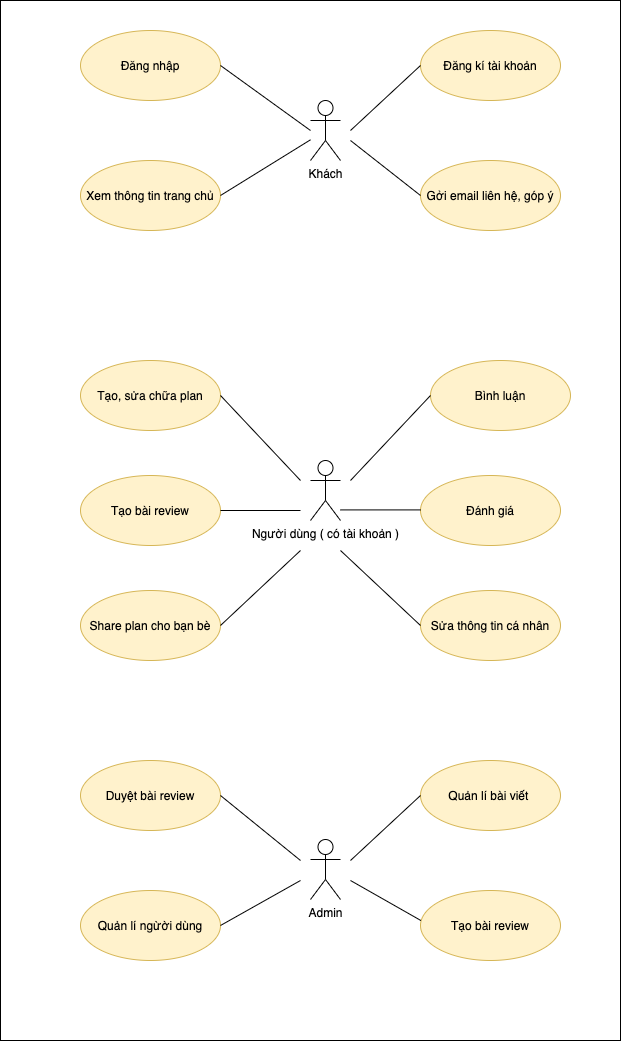
\includegraphics[width=14cm]{document/image/List3ND.png}
  \captionof{figure}{Lược đồ Usecase các đối tượng của hệ thống }
\end{center}
% \subsection{Đối tượng: Quản trị hệ thống}
% \textbf{Lược đồ Usecase đối tượng quản trị hệ thống}
% \begin{center}
%   \captionsetup{type=figure}
%   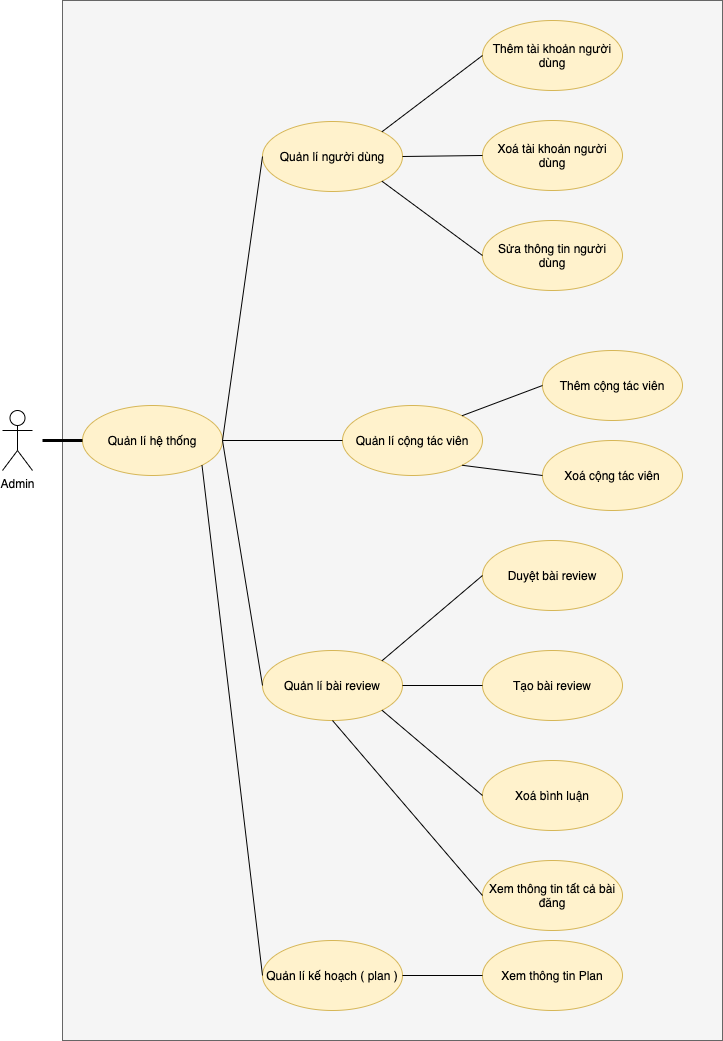
\includegraphics[width=13cm]{document/image/useCaseAdmin.png}
%   \captionof{figure}{Lược đồ usecase của đối tượng quản trị hệ thống}
% \end{center}

% \indent Đối với đối tượng là quản trị hệ thống, sau khi xác thực thành công sẽ có những nhóm chức năng: quản lí người dùng, quản lí cộng tác viên, quản lí bài review và quản lí kế hoạch. Với mỗi nhóm chức năng sẽ có những chức năng tương ứng sau:

% \begin{itemize}
%     \item Nhóm quản lý tài khoản người dùng & tài khoản cộng tác viên bao gồm các chức năng:
%         \subitem - Xem thông tin các tài khoản.
%         \subitem - Tạo mới tài khoản.
%         \subitem - Xoá tài khoản người dùng.
%         \subitem - Chỉnh sửa thông tin tài khoản.
%         \subitem - Thêm và xoá vai trò cho tài khoản.
    
%     \item Nhóm quản lý bài review:
%         \subitem - Phê duyệt bài review người dùng đăng.
%         \subitem - Xem danh sách tất cả các bài viết.
%         \subitem - Tạo mới và xoá bài viết.
%         \subitem - Quản lí bình luận người dùng.
%         \subitem - Duyệt bài viết người dùng.
%     \item Chắc năng quản lí kế hoạch chỉ cho phép quản lí hệ thống chỉ có thể xem thông tin các kế hoạch mà người dùng đã tạo mà không thể can thiệp quá sâu.
%     \item Ngoài ra nhóm quản lí có thể cấu hình giao diện trang chủ, cấu hình thông tin trang web, cấu hình email cho hệ thống.
%         \subitem - Cấu hình giao diện trang chủ: Tùy chỉnh các thành phần giao diện, lựa chọn các thành phần giao diện sẽ xuất hiện ở trang chủ.
%         \subitem - Cấu hình thông tin trang web: Cấu hình các thông tin chung cho hệ thống.
%         \subitem - Cấu hình email hệ thống: Tủy chỉnh các mẫu email tự động của hệ thống.
% \end{itemize}
\subsection{Đối tượng: Khách}
\textbf{Lược đồ Usecase đối tượng khách}
\begin{center}
  \captionsetup{type=figure}
  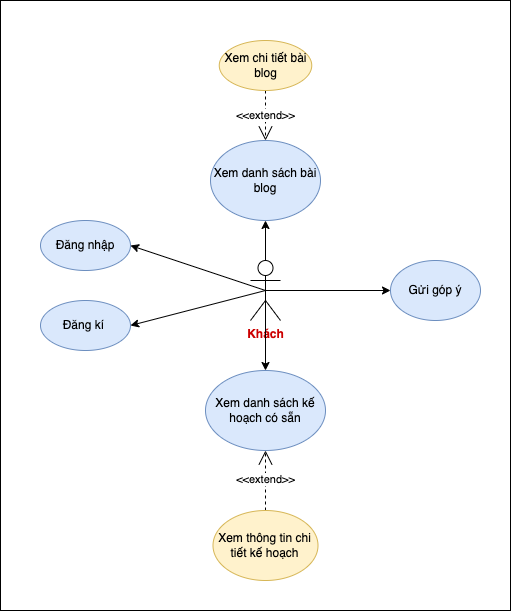
\includegraphics[width=14cm]{document/image/usecaseKhach2.png}
  \captionof{figure}{Lược đồ Usecase của đối tượng khách}
\end{center}

Khách là những người dùng chưa đăng nhập, bao gồm tất cả các đối tượng như học sinh,  sinh viên, phụ huynh, đơn vị, doanh nghiệp là đối tác của Website,...
 
 Đối tượng khách có thể truy cập trang chủ để xem các thông tin chung, thông tin liên hệ, xem các tin tức và sự kiện, bài review, thông tin chuyến đi. Khi có nhu cầu liên hệ với Goz, khách có thể vào mục liên hệ để gửi email để liên lạc hoạt gọi hotline để được hỗ trợ trực tiếp.
 
\clearpage
\subsection{Đối tượng: Người dùng ( đã có tài khoản )}
\textbf{Lược đồ Usecase đối tượng người dùng}
\begin{center}
  \captionsetup{type=figure}
  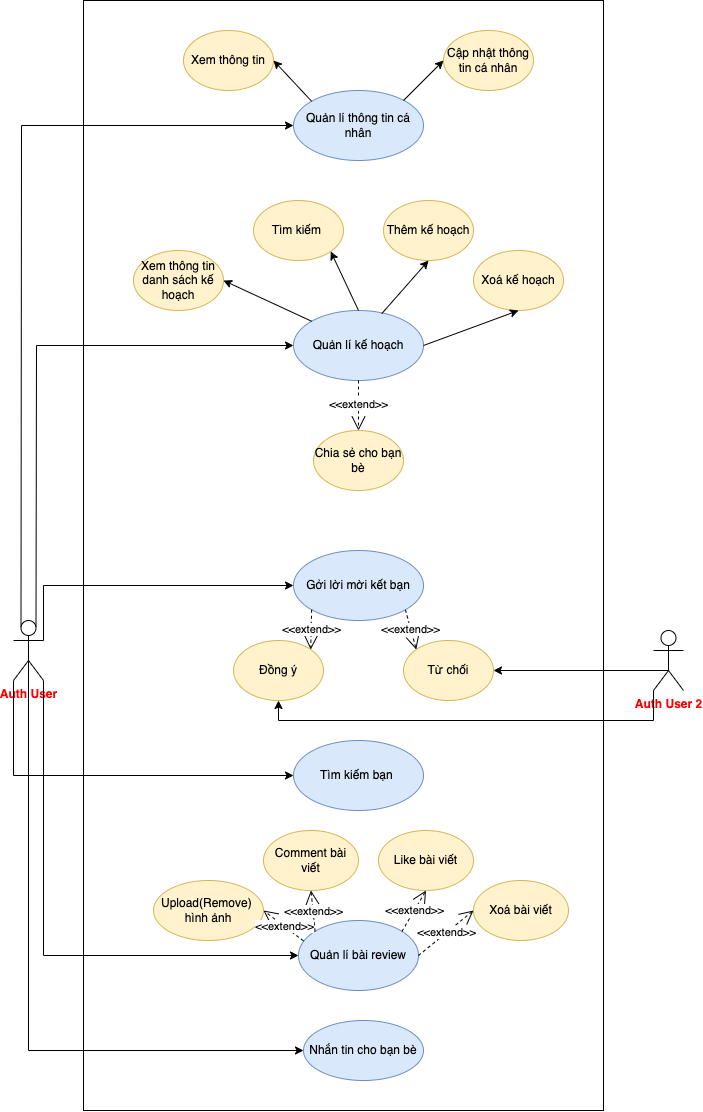
\includegraphics[width=14cm]{document/image/usecaseAuthUser.drawio.png}
  \captionof{figure}{Lược đồ Usecase đối tượng người dùng}
\end{center}

Đối với người dùng đã có tài khoản đăng nhập, sau khi đăng nhập sẽ  có các chức năng như sau: 
\begin{itemize}
    \item Quản lí thông tin cá nhân:
        \subitem - Xem và sửa các thông tin cá nhân.
    \item Quản lí kế hoạch:
        \subitem - Xem và sửa các thông tin kế hoạch chuyến đi.
        \subitem - Tạo kế hoạch mới.
        \subitem - Xoá kế hoạch.
        \subitem - Chia sẻ kế hoạch với bạn bè.
        
    \item Quản lí bài review:
        \subitem - Tạo bài review mới.
        \subitem - Bình luận bài review.
        \subitem - Thích bài review
        \subitem - Đánh giá.
    \item Tương tác với người dùng khác: 
    \subitem - Tìm kiếm bạn bè.
    \subitem - Gởi lời mời kết bạn.
    \subitem - Đồng ý hoặc từ chối lời mời kết bạn từ người khác.
    \subitem - Nhắn tin cho bạn bè.
     
    
\end{itemize}

\clearpage
% \subsection{Đối tượng: Quản lý ( admin )}
% \textbf{Lược đồ Usecase đối tượng quản lý}
% \begin{center}
%   \captionsetup{type=figure}
%   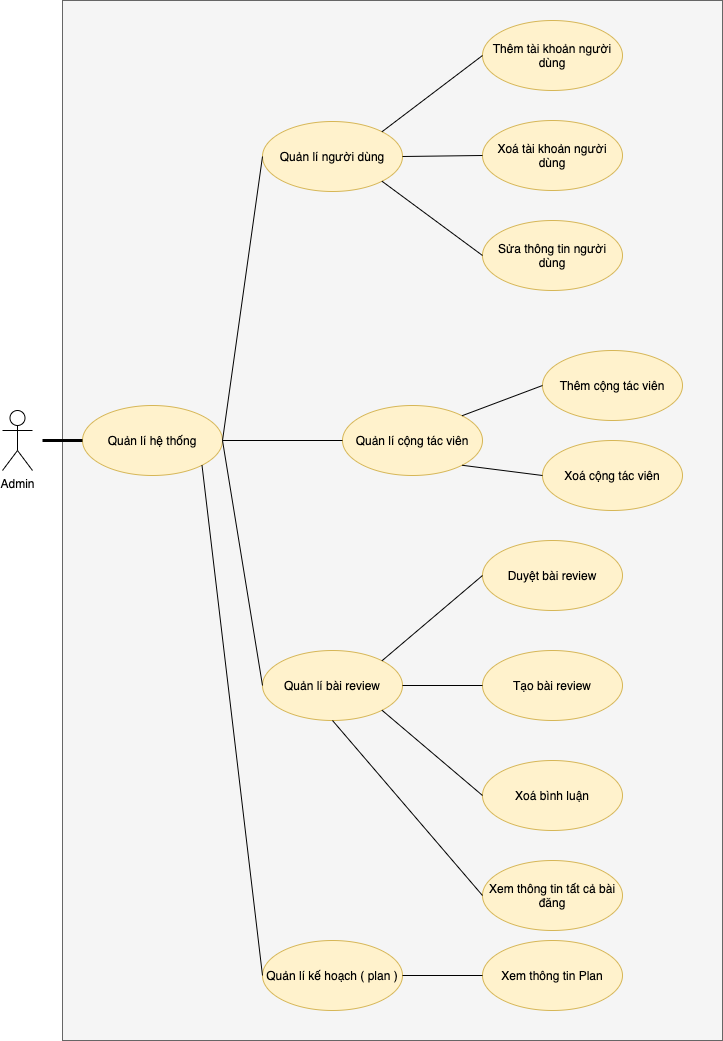
\includegraphics[width=15cm]{document/image/useCaseAdmin.png}
%   \captionof{figure}{Lược đồ Usecase đối tượng quản lý ( admin )}
% \end{center}

% Sau khi đăng nhập vào hệ thống, người dùng là quản lý sẽ có các nhóm chức năng sau: quản lý, tạo và đăng bài review các địa điểm du lịch mới. Phê duyệt bài review do người dùng đăng.

% Chức năng quản lý bài review bao gồm xem danh sách toàn bộ bài review, tạo mới, sửa đổi và xoá bài review.

% Chức năng quản lí cộng tác viên bao gồm thêm ( xoá ) tài khoản cộng tác viên như chủ khách sạn, homestay, nhà hàng, ... .

% Chức năng quản lí kế hoạch ( plan ) chỉ có thể xem thông tin kế hoạch mà người dùng đã tạo.

% \clearpage

\section{Thiết kế cơ sở dữ liệu cho hệ thống}
\subsection{Lược đồ ERD}

Chi tiết xem ở tài liệu đính kèm.

\subsection{Lược đồ cơ sở dữ liệu}
\begin{center}
  \captionsetup{type=figure}
g  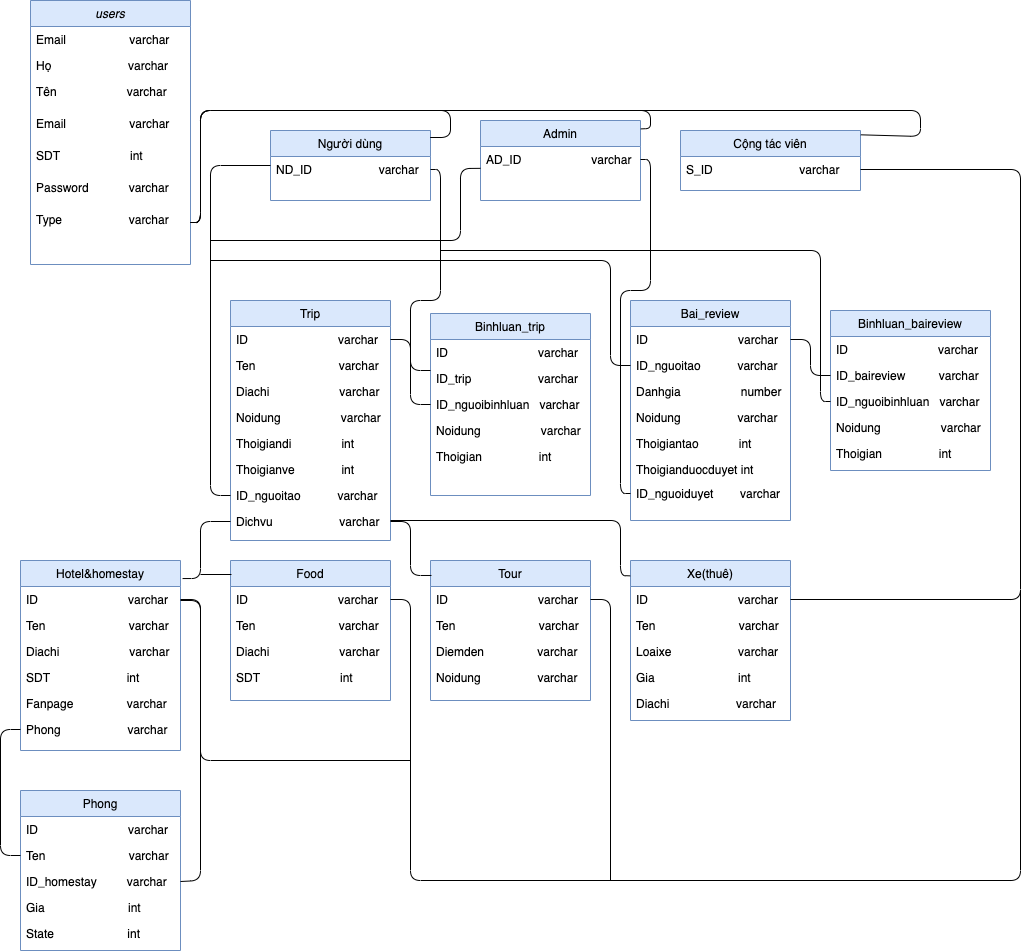
\includegraphics[width=\linewidth]{image/classDiagram.png}
  \captionof{figure}{Thiết kế cơ sở dữ liệu của hệ thống}
\end{center}
\section{Chức năng từng đối tượng trong hệ thống}
Từ việc thiết kế Usecase ở chương 4, nhóm nghiên cứu tiến hành thực hiện từng chức năng tương ứng với mỗi đối tượng. Cụ thể từng chức năng quan trọng như sau:

\subsection{Chức năng đăng kí tài khoản cá nhân.}\\
 Đặc tả usecase đăng ký tài khoản cá nhân:  

\begin{table}[H]
    \centering
	\begin{tabular}{|p{5cm}|p{10cm}|}
    % \hline
    % \textbf{Người dùng}&\textbf{Đặc tả}\\
    \hline
    Usecase Name&Đăng ký tài khoản cá nhân\\
    \hline
    Usecase Description&Người dùng muốn đăng kí tài khoản cá nhân\\
    \hline
    Post Condition&Hiển thị thông báo thành công và chuyển đến trang đăng nhập\\
    \hline
    Basic Flow& 1. Người dùng nhấn vào nút "Đăng ký" ở thanh sidebar.
    
    2. Chuyển đến trang đăng ký.
    
    3. Nhập họ tên.
    
    4. Nhập email.
    
    5. Nhập mật khẩu.
    
    6. Nhập lại mật khẩu.
    
    7. Nhập số điện thoại.
    
    8. Nhập ngày tháng năm sinh.
    
    9. Chọn giới tính.
    
    10. Nhập địa chỉ.
    
    11. Nhấn nút đăng ký.\\
    \hline Business Rules&- Email là duy nhất.
    
    - Số điện thoại đúng chuẩn và duy nhất.\\
   
   
	\hline
\end{tabular}
\caption{Usecase đăng ký tài khoản }
\end{table}

\begin{center}
    \captionsetup{type=figure}
    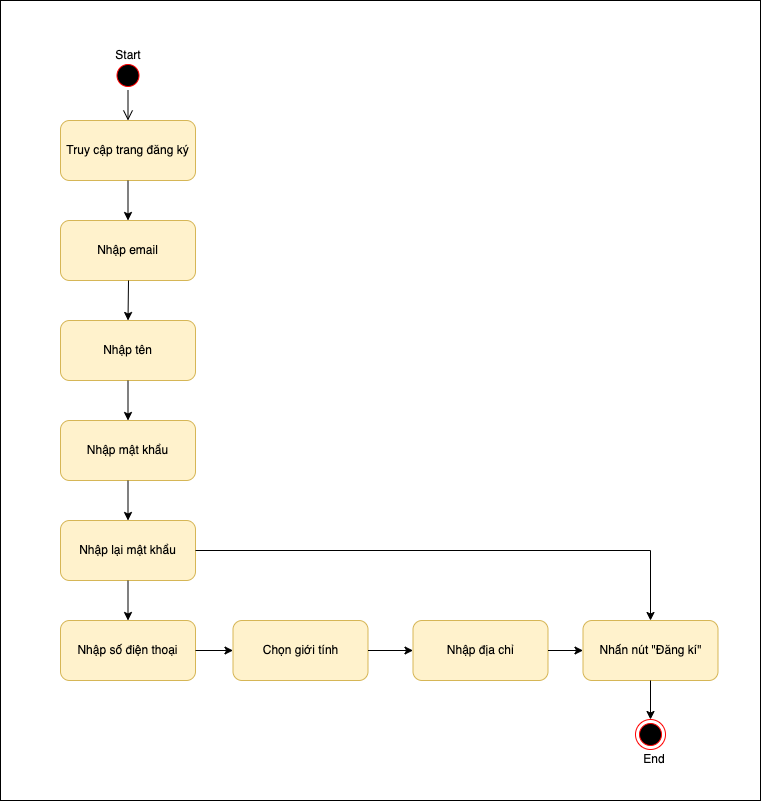
\includegraphics[width=12cm]{document/image/activityDK.drawio.png}
    \captionof{figure}{Lược đồ Activity đăng kí }
\end{center}

\subsection{Chức năng Lên kế hoạch và tạo chi tiết thông tin chuyến đi}
 Đặc tả usecase tạo kế hoạch:  
 \begin{table}[H]
    \centering
	\begin{tabular}{|p{5cm}|p{10cm}|}
    % \hline
    % \textbf{Người dùng}&\textbf{Đặc tả}\\
    \hline
    Usecase Name&Tạo kế hoạch chi tiết cho chuyến đi\\
    \hline
    Usecase Description&Người dùng muốn tạo kế hoạch chi tiết cho chuyến đi\\
    \hline
    Post Condition&Hiển thị thông báo thành công \\
    \hline
    Basic Flow& 1. Người dùng nhấn vào nút "Create Plan" ở thanh sidabar
    
    2. Chuyển đến trang tạo kế hoạch.
    
    3. Nhập ngày đi.
    
    4. Nhập ngày về
    
    5. Nhập địa điểm đến
    
    6. Nhấn nút "Create".
    
    7. Chuyển đến giao diện tất cả kế hoạch tính theo số ngày đi.
    
    8. Chọn kế hoạch muốn thêm hoạt động.
    
    9. Chuyển đến giao diện thêm hoạt động chi tiết cho chuyến đi.
    
    10. Nhập thời gian
    
    11. Chọn thể loại hoạt động.
    
    12. Chọn địa điểm cho hoạt động đó.
    
    13. Nhấn nút "Add"\\
    \hline Business Rules&- \\
   
   
	\hline
\end{tabular}
\caption{Usecase tạo kế hoạch }
\end{table}
 \begin{center}
  \captionsetup{type=figure}
  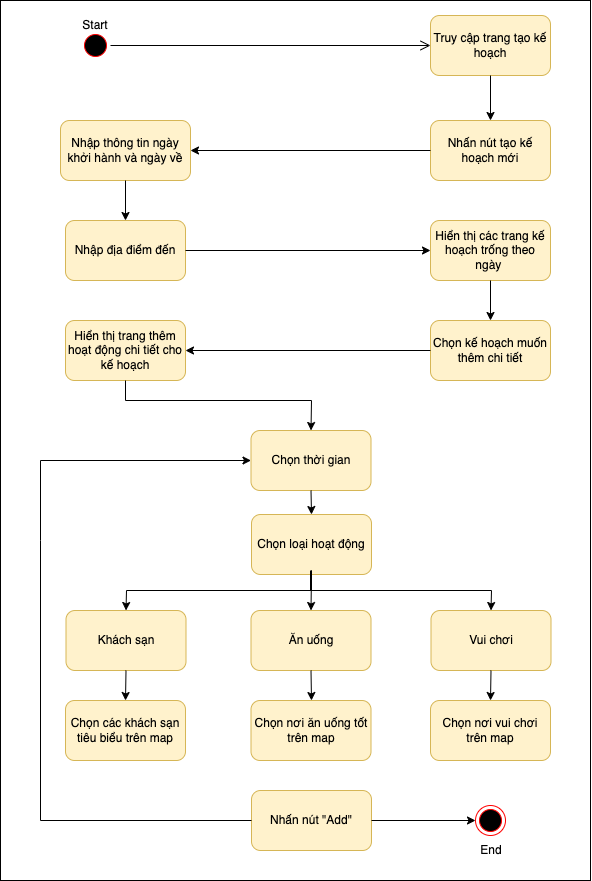
\includegraphics[width=12cm]{document/image/usecasePlan.drawio.png}
  \captionof{figure}{Lược đồ Activity tạo thông tin kế hoạch cho chuyến đi}
\end{center}

\subsection{Chức năng tạo vài blog về địa điểm vừa đi}

Đặc tả usecase tạo bài blog: 
\begin{table}[H]
    \centering
	\begin{tabular}{|p{5cm}|p{10cm}|}
    % \hline
    % \textbf{Người dùng}&\textbf{Đặc tả}\\
    \hline
    Usecase Name&Tạo bài blog\\
    \hline
    Usecase Description&Người dùng muốn tạo bài blog\\
    \hline
    Post Condition&Hiển thị thông báo thành công \\
    \hline
    Basic Flow& 1. Người dùng nhấn vào nút "Create Blog" ở thanh sidebar
    
    2. Chuyển đến trang tạo blog.
    
    3. Nhập địa điểm đã đi
    
    4. Upload hình ảnh
    
    5. Nhập trải nghiệm.
    
    6. Nhấn nút "Create".
    
    7. Thông báo thành công.\\
    

    \hline Business Rules& \\
   
   
	\hline
\end{tabular}
\caption{Usecase tạo bài blog }
\end{table}
 \begin{center}
  \captionsetup{type=figure}
  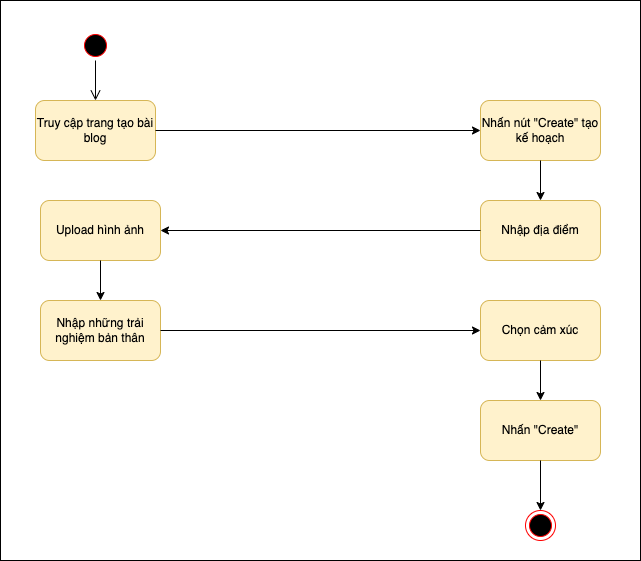
\includegraphics[width=12cm]{document/image/usecaseBlog.drawio.png}
  \captionof{figure}{Lược đồ Activity tạo bài blog}
\end{center}

\subsection{Chức năng kết bạn}
Đặc tả usecase kết bạn: 
\begin{table}[H]
    \centering
	\begin{tabular}{|p{5cm}|p{10cm}|}
    
    \hline
    Usecase Name&Kết bạn\\
    \hline
    Usecase Description&Người dùng muốn kết bạn với người dùng khác\\
    \hline
    Post Condition&Hiển thị thông báo gởi lời mời kết bạn thành công \\
    \hline
    Basic Flow& 1. Người dùng nhấn vào biểu tượng kết bạn hoặc nhấn vào ô "Search" để tìm người mình muốn kết bạn.
    
    2. Nhập tên người dùng muốn kết bạn.
    
    3. Nhấn "Add"
    
    4. Hiển thị thông bảo thành công\\
    

    \hline Business Rules& \\
   
   
	\hline
\end{tabular}
\caption{Usecase kết bạn}
\end{table}
 \begin{center}
  \captionsetup{type=figure}
  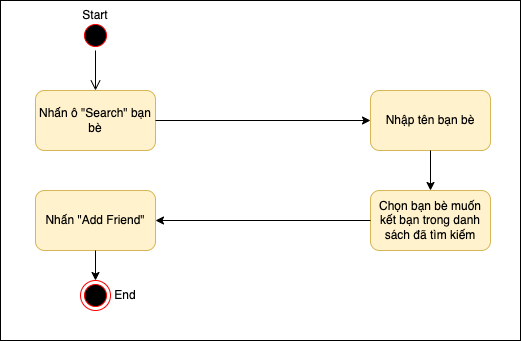
\includegraphics[width=12cm]{document/image/KetBan.drawio.png}
  \captionof{figure}{Lược đồ Activity kết bạn}
\end{center}

\subsection{Chức năng đồng ý và từ chối lời mời kết bạn}
Đặc tả usecase đồng ý và từ chối lời mời kết bạn: 
\begin{table}[H]
    \centering
	\begin{tabular}{|p{5cm}|p{10cm}|}
    
    \hline
    Usecase Name&Đồng ý hoặc từ chối lời mời kết bạn\\
    \hline
    Usecase Description&Người dùng muốn phản hồi lời mời kết bạn\\
    \hline
    Post Condition&Hiển thị thông báo chấp nhận ( từ chối ) lời mời thành công \\
    \hline
    Basic Flow& 1. Người dùng nhấn vào biểu tượng bạn bè trên thanh sidebar
    2. Hiển thị danh sách người dùng đã gởi lời mời kết bạn.
    
    3. Nhấn "Accecpt" để đồng ý hoặc "Decline" để từ chối.
    
    4. Hiển thị thông bảo thành công\\
    

    \hline Business Rules& \\
   
   
	\hline
\end{tabular}
\caption{Usecase đồng ý hoặc từ chối lời mời kết bạn}
\end{table}
 \begin{center}
  \captionsetup{type=figure}
  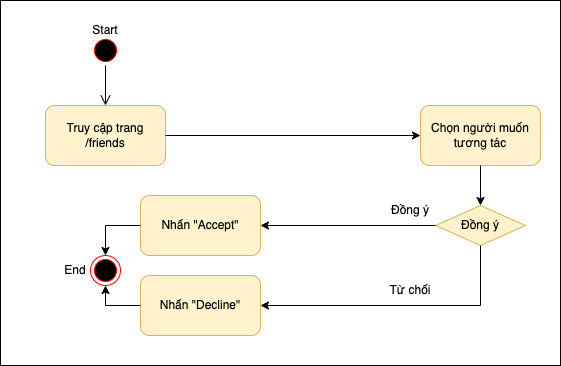
\includegraphics[width=12cm]{document/image/acKetban.drawio.png}
  \captionof{figure}{Lược đồ Activity đồng ý hoặc từ chối lời mời kết bạn}
\end{center}

\subsection{Chức năng Unfriend bạn}
Đặc tả usecase unfriend bạn: 
\begin{table}[H]
    \centering
	\begin{tabular}{|p{5cm}|p{10cm}|}
    
    \hline
    Usecase Name&Unfriend bạn\\
    \hline
    Usecase Description&Người dùng muốn xoá quan hệ bạn bè\\
    \hline
    Post Condition&Hiển thị thông báo xoá bạn bè thành công. \\
    \hline
    Basic Flow& 1. Người dùng nhấn vào ô "Search" để tìm bạn bè muốn unfriend.
    2. Hiển thị danh sách người dùng có tên vừa tìm kiếm.
    
    3. Chọn bạn bè muốn huỷ quan hệ bạn bè.
    
    4. Nhấn "Unfriend".
    
    5. Hiển thi thông báo thành công.\\
    

    \hline Business Rules& \\
   
   
	\hline
\end{tabular}
\caption{Usecase huỷ quan hệ bạn bè}
\end{table}
 \begin{center}
  \captionsetup{type=figure}
  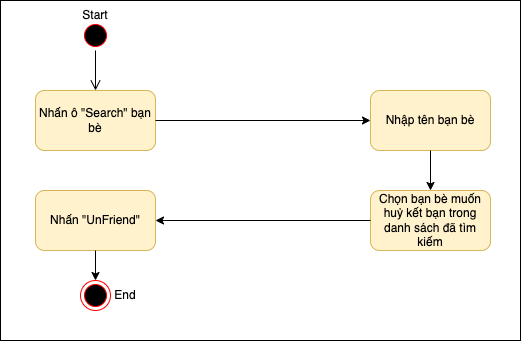
\includegraphics[width=12cm]{document/image/Unfriend.png}
  \captionof{figure}{Lược đồ Activity huỷ kết bạn}
\end{center}

\subsection{Chức năng nhắn tin với bạn bè}
Đặc tả usecase nhắn tin với bạn: 
\begin{table}[H]
    \centering
	\begin{tabular}{|p{5cm}|p{10cm}|}
    
    \hline
    Usecase Name&Nhắn tin với bạn bè\\
    \hline
    Usecase Description&Người dùng muốn nhắn tin với bạn bè\\
    \hline
    Post Condition&Hiển thị thông báo gởi tin nhắn thành công \\
    \hline
    Basic Flow& 1. Người dùng nhấn vào biểu tượng "Chat" trên thanh sidebar
    2. Hiển thị danh sách bạn bè.
    
    3. Chọn bạn bè muốn nhắn tin.
    
    4. Nhập thông tin cuộc hội thoại.
    
    5. Nhấn "Gửi"
    
    5. Hiển thi thông báo gửi tin nhắn thành công.\\
    

    \hline Business Rules& \\
   
   
	\hline
\end{tabular}
\caption{Usecase nhắn tin}
\end{table}
 \begin{center}
  \captionsetup{type=figure}
  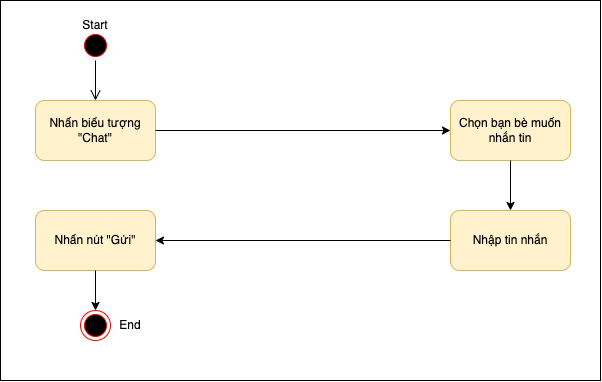
\includegraphics[width=12cm]{document/image/Chat.png}
  \captionof{figure}{Lược đồ Activity nhắn tin}
\end{center}

\subsection{Chức năng chia sẻ kế hoạch với bạn bè}
Đặc tả usecase chia sẻ kế hoạch với bạn bè: 
\begin{table}[H]
    \centering
	\begin{tabular}{|p{5cm}|p{10cm}|}
    
    \hline
    Usecase Name&Share kế hoạch với bạn bè\\
    \hline
    Usecase Description&Người dùng muốn share kế hoạch của mình với bạn bè\\
    \hline
    Post Condition&Hiển thị thông báo share thành công \\
    \hline
    Basic Flow& 1. Người dùng vào trang các kế hoạch đã tạo.
    
    2. Hiển thị danh sách các kế hoạch đã tạo.
    
    3. Nhấn vào biểu tượng "Share" trên bài.
    
    4. Hiển thị danh sách bạn bè.
    
    5. Nhấn chọn bạn bè muốn gởi.
    
    6. Nhấn "Share".
    
    5. Hiển thi thông báo thành công.\\
    

    \hline Business Rules& \\
   
   
	\hline
\end{tabular}
\caption{Usecase share kế hoạch}
\end{table}
 \begin{center}
  \captionsetup{type=figure}
  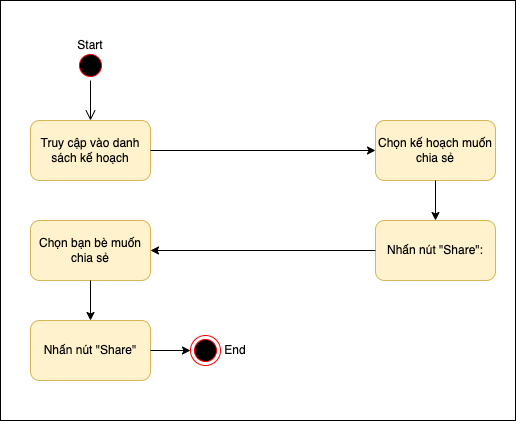
\includegraphics[width=12cm]{document/image/Share.png}
  \captionof{figure}{Lược đồ Activity share kế hoạch}
\end{center}
% \begin{figure}[H]
%     \centering
%     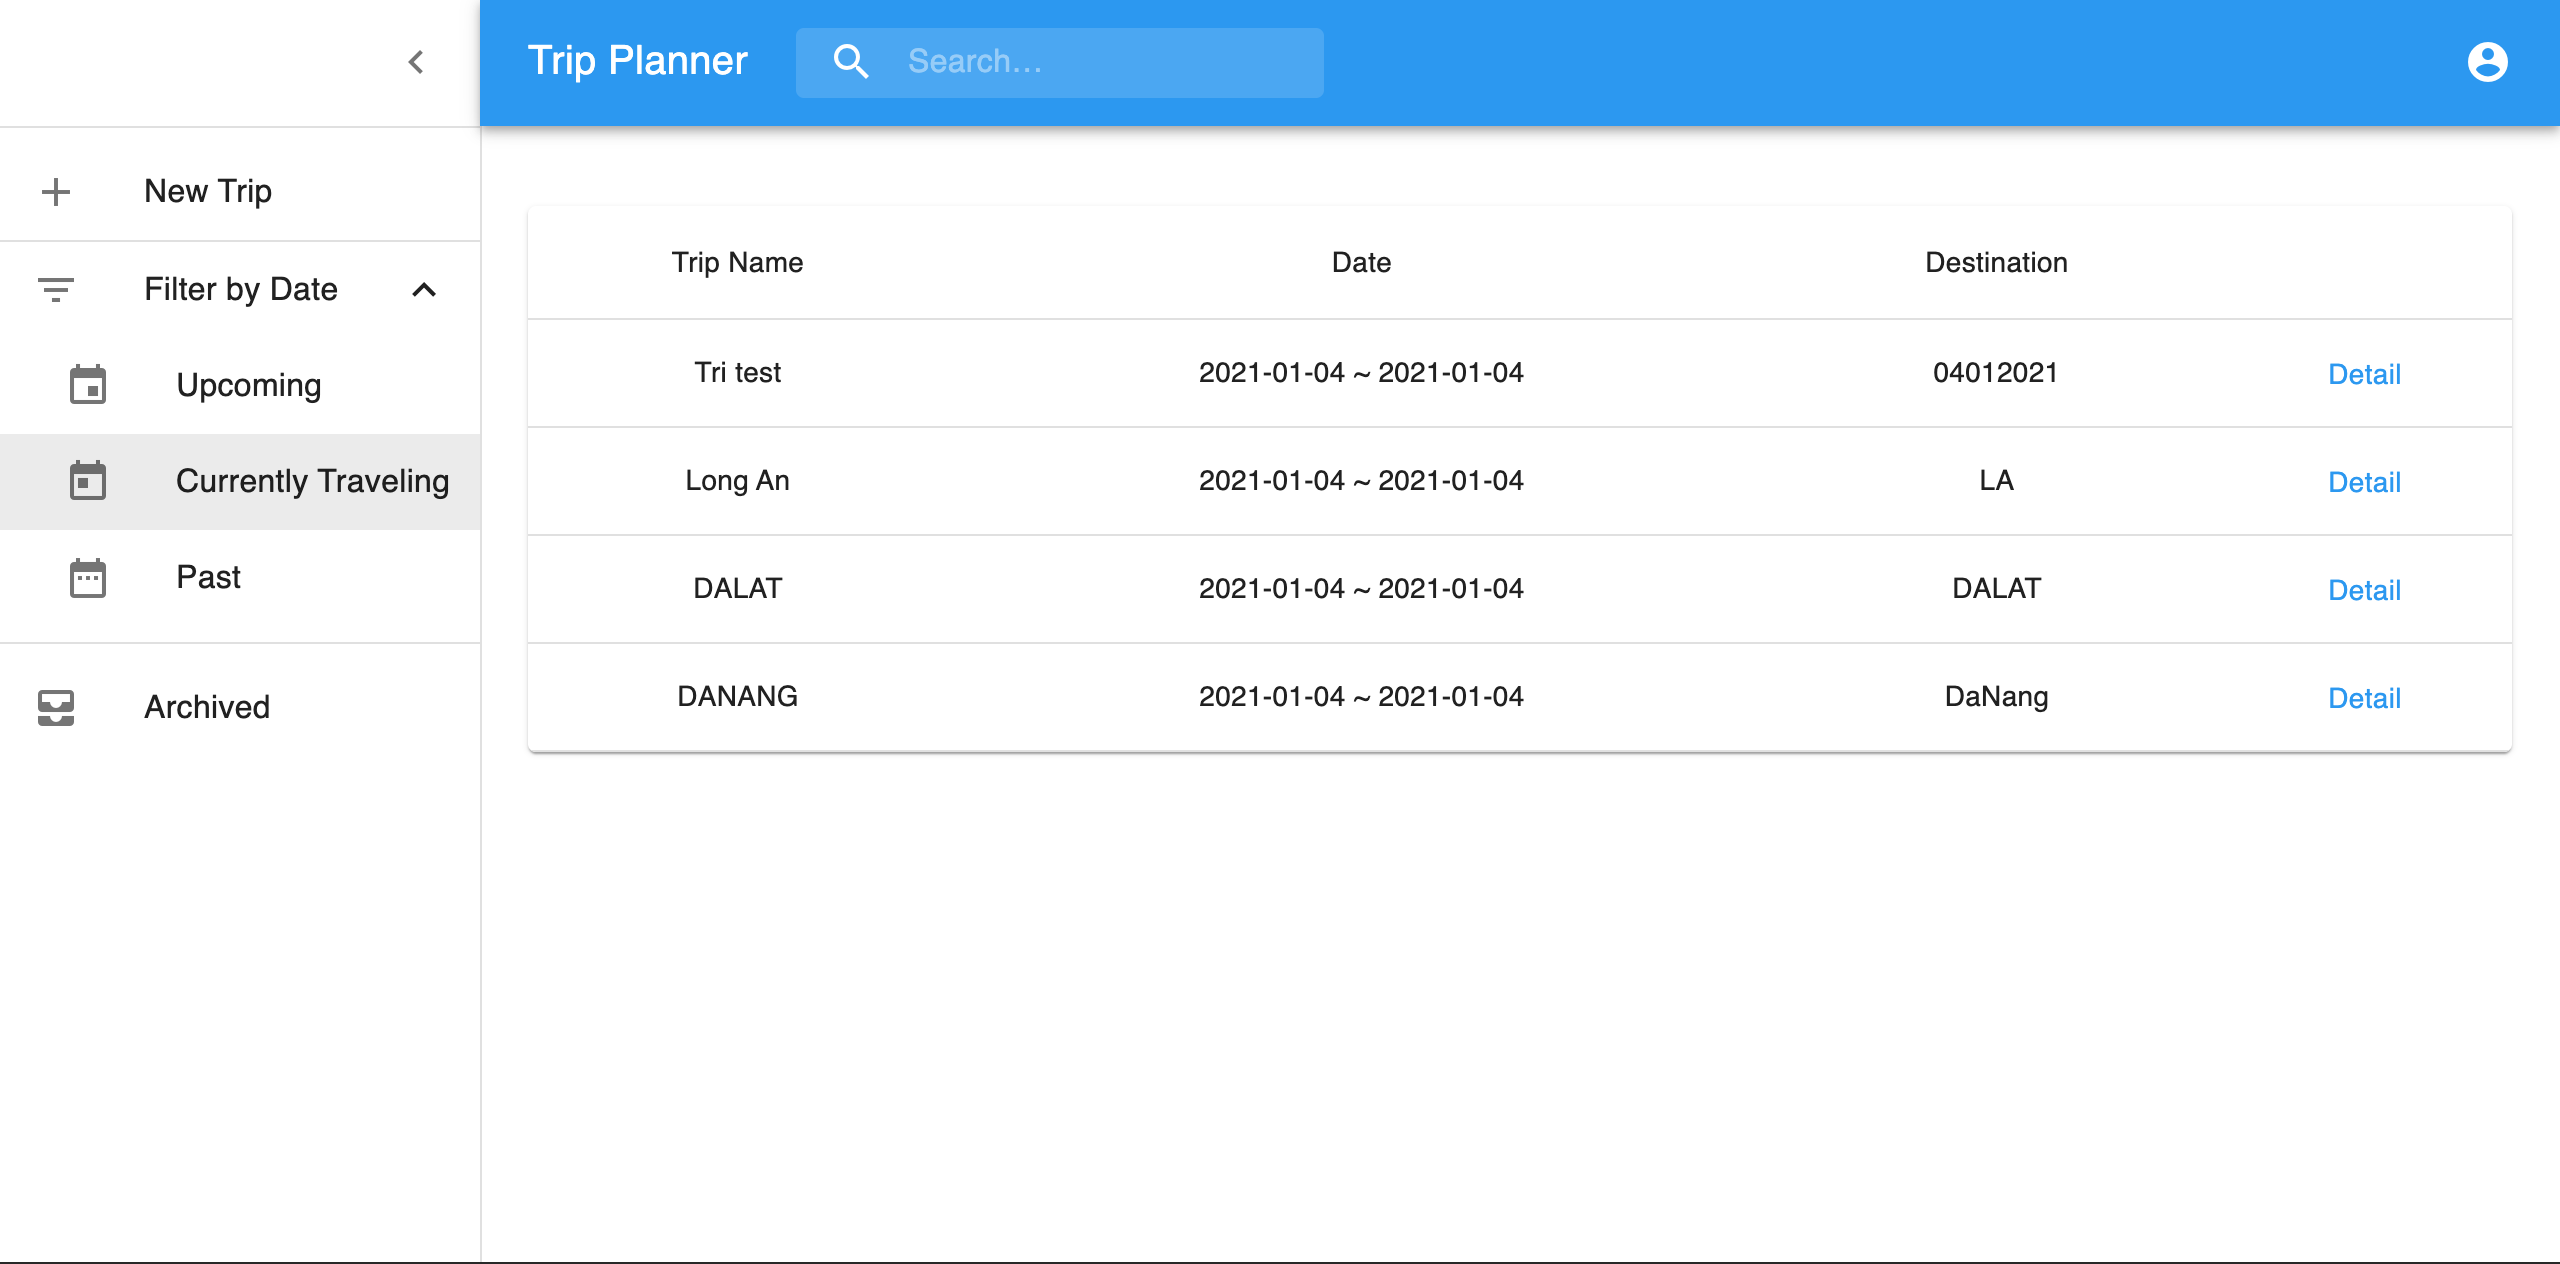
\includegraphics[width=15cm]{document/image/BangPlan.png}
%     \caption{Danh sách kế hoạch hiện có của người dùng}
%     \label{fig:fig_danh_sach_nguoi_dung}
% \end{figure}
 
% Danh sạch kế hoạch hiện có giúp người dùng có thể tự quản lý kế hoạch của mình cũng như các kế hoạch mình đã tham gia ( Past ). Người dùng có thể thêm xoá và sửa chữa thông tin trong kế hoạch của mình\\
% \begin{figure}[H]
%     \centering
%     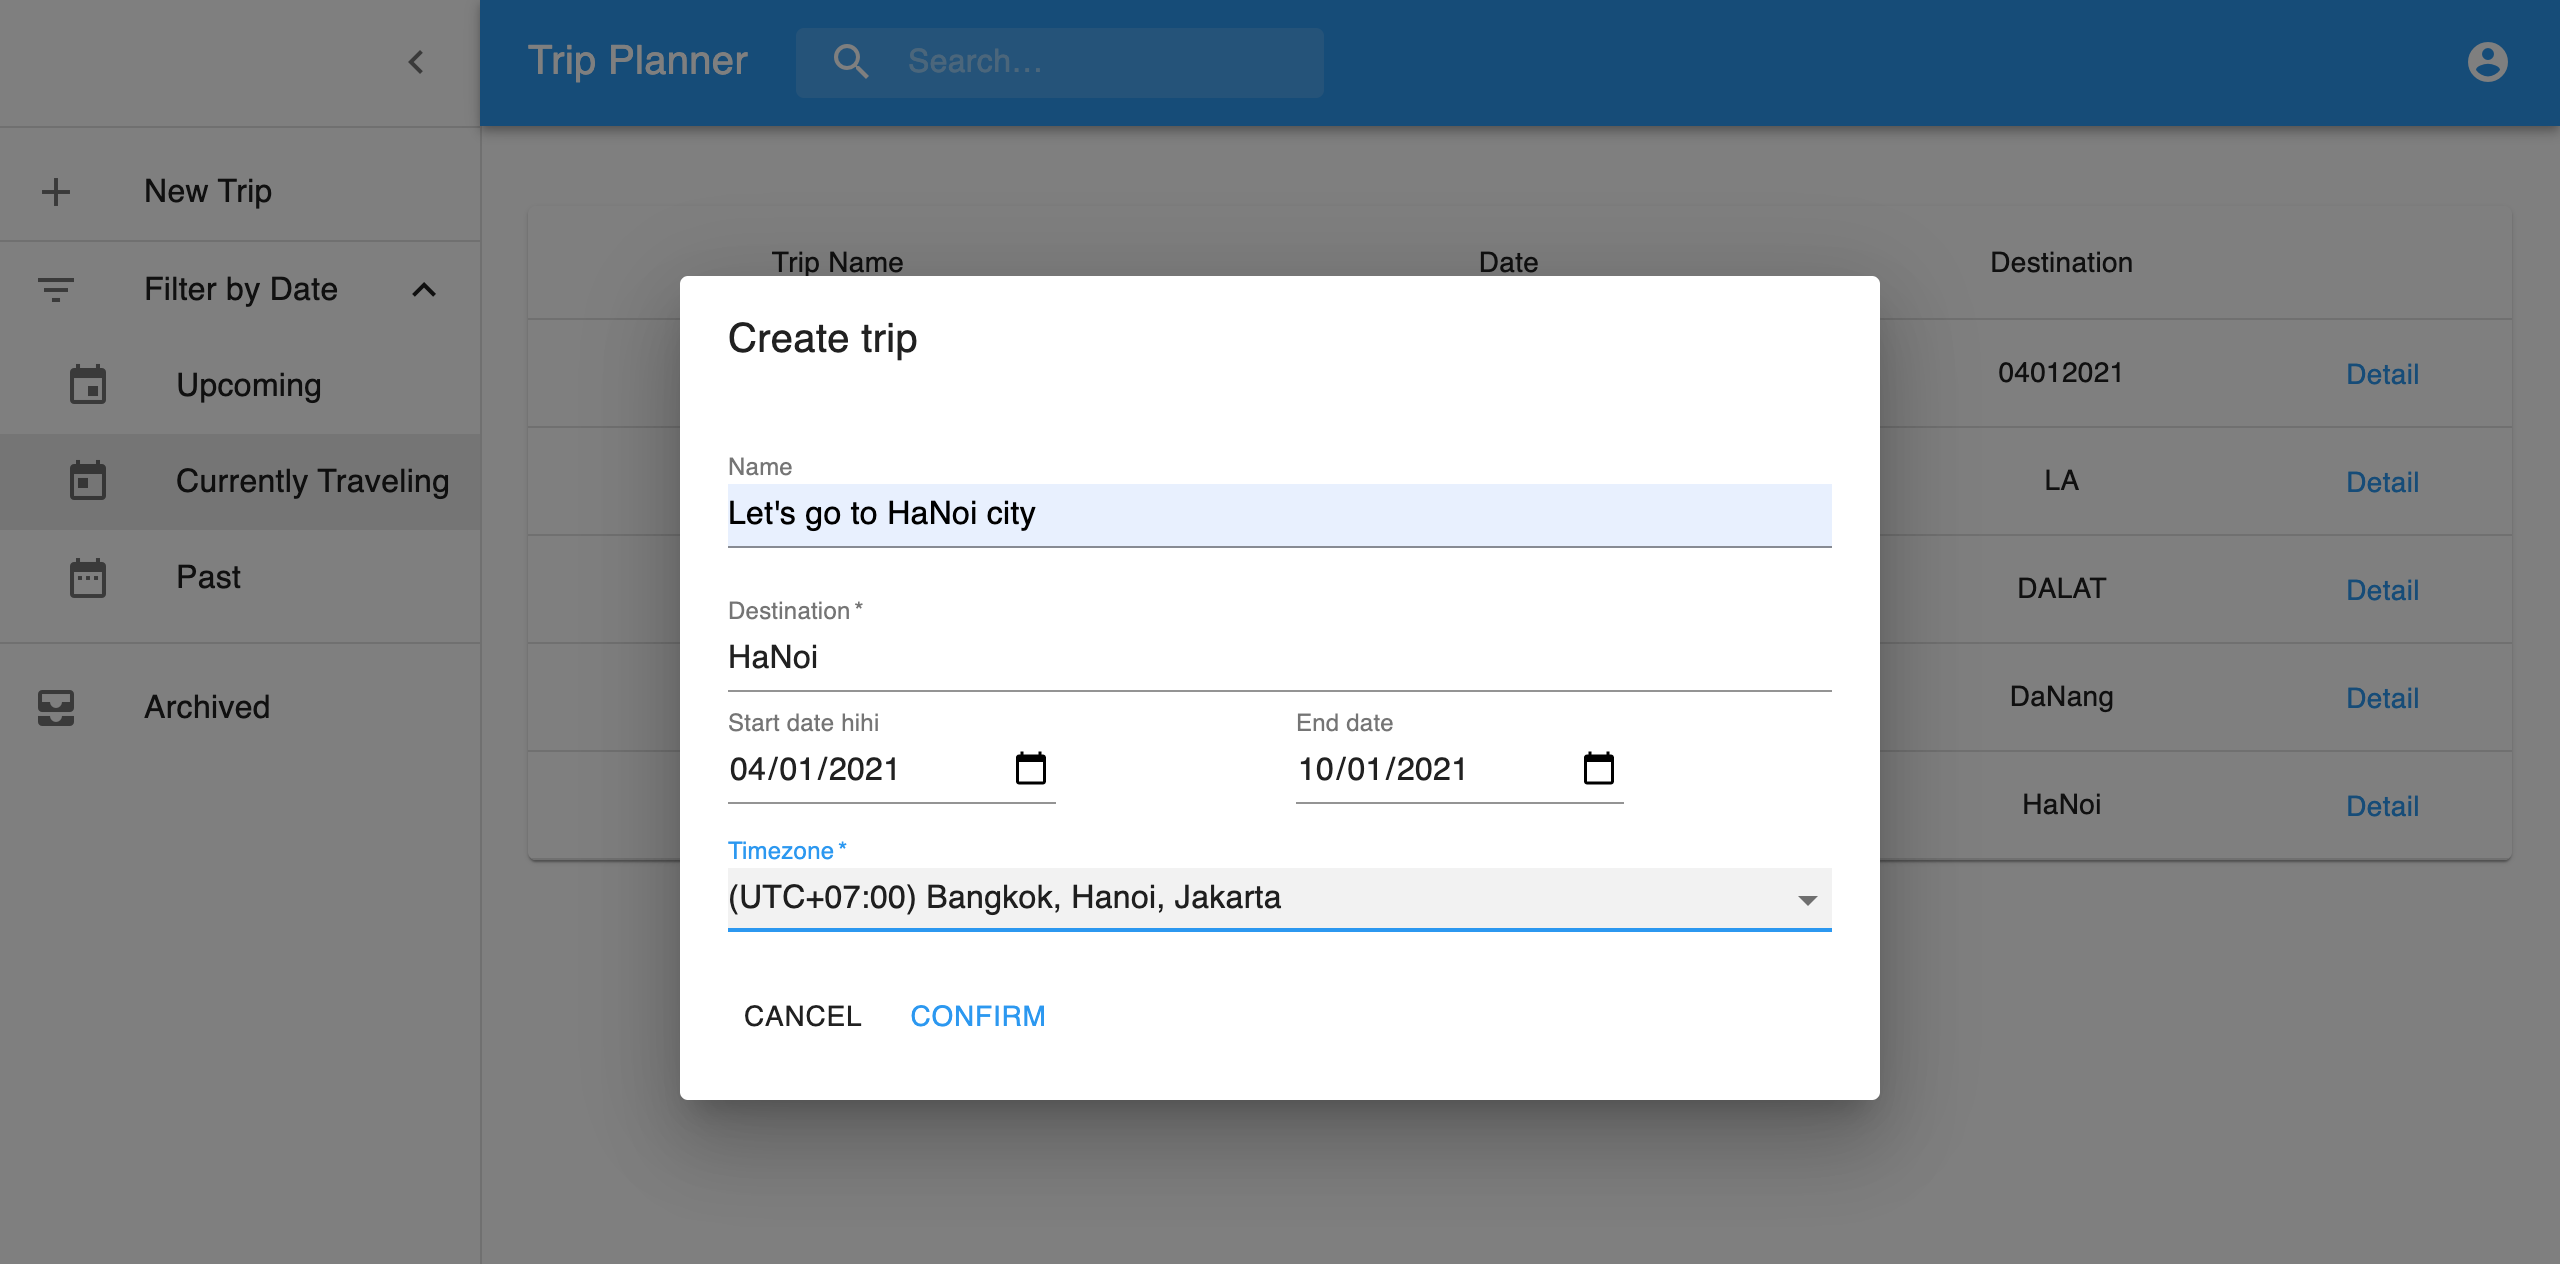
\includegraphics[width=15cm]{document/image/CreateNewPlan.png}
%     \caption{Thêm kế hoạch mới}
%     \label{fig:fig_edit_nguoi_dung}
% \end{figure}

% Khi đã tạo kế hoạch cho chuyến đi, người dùng có thể thêm các hoạt động chi tiết cho mỗi ngày đi \\

% \begin{figure}[H]
%     \centering
%     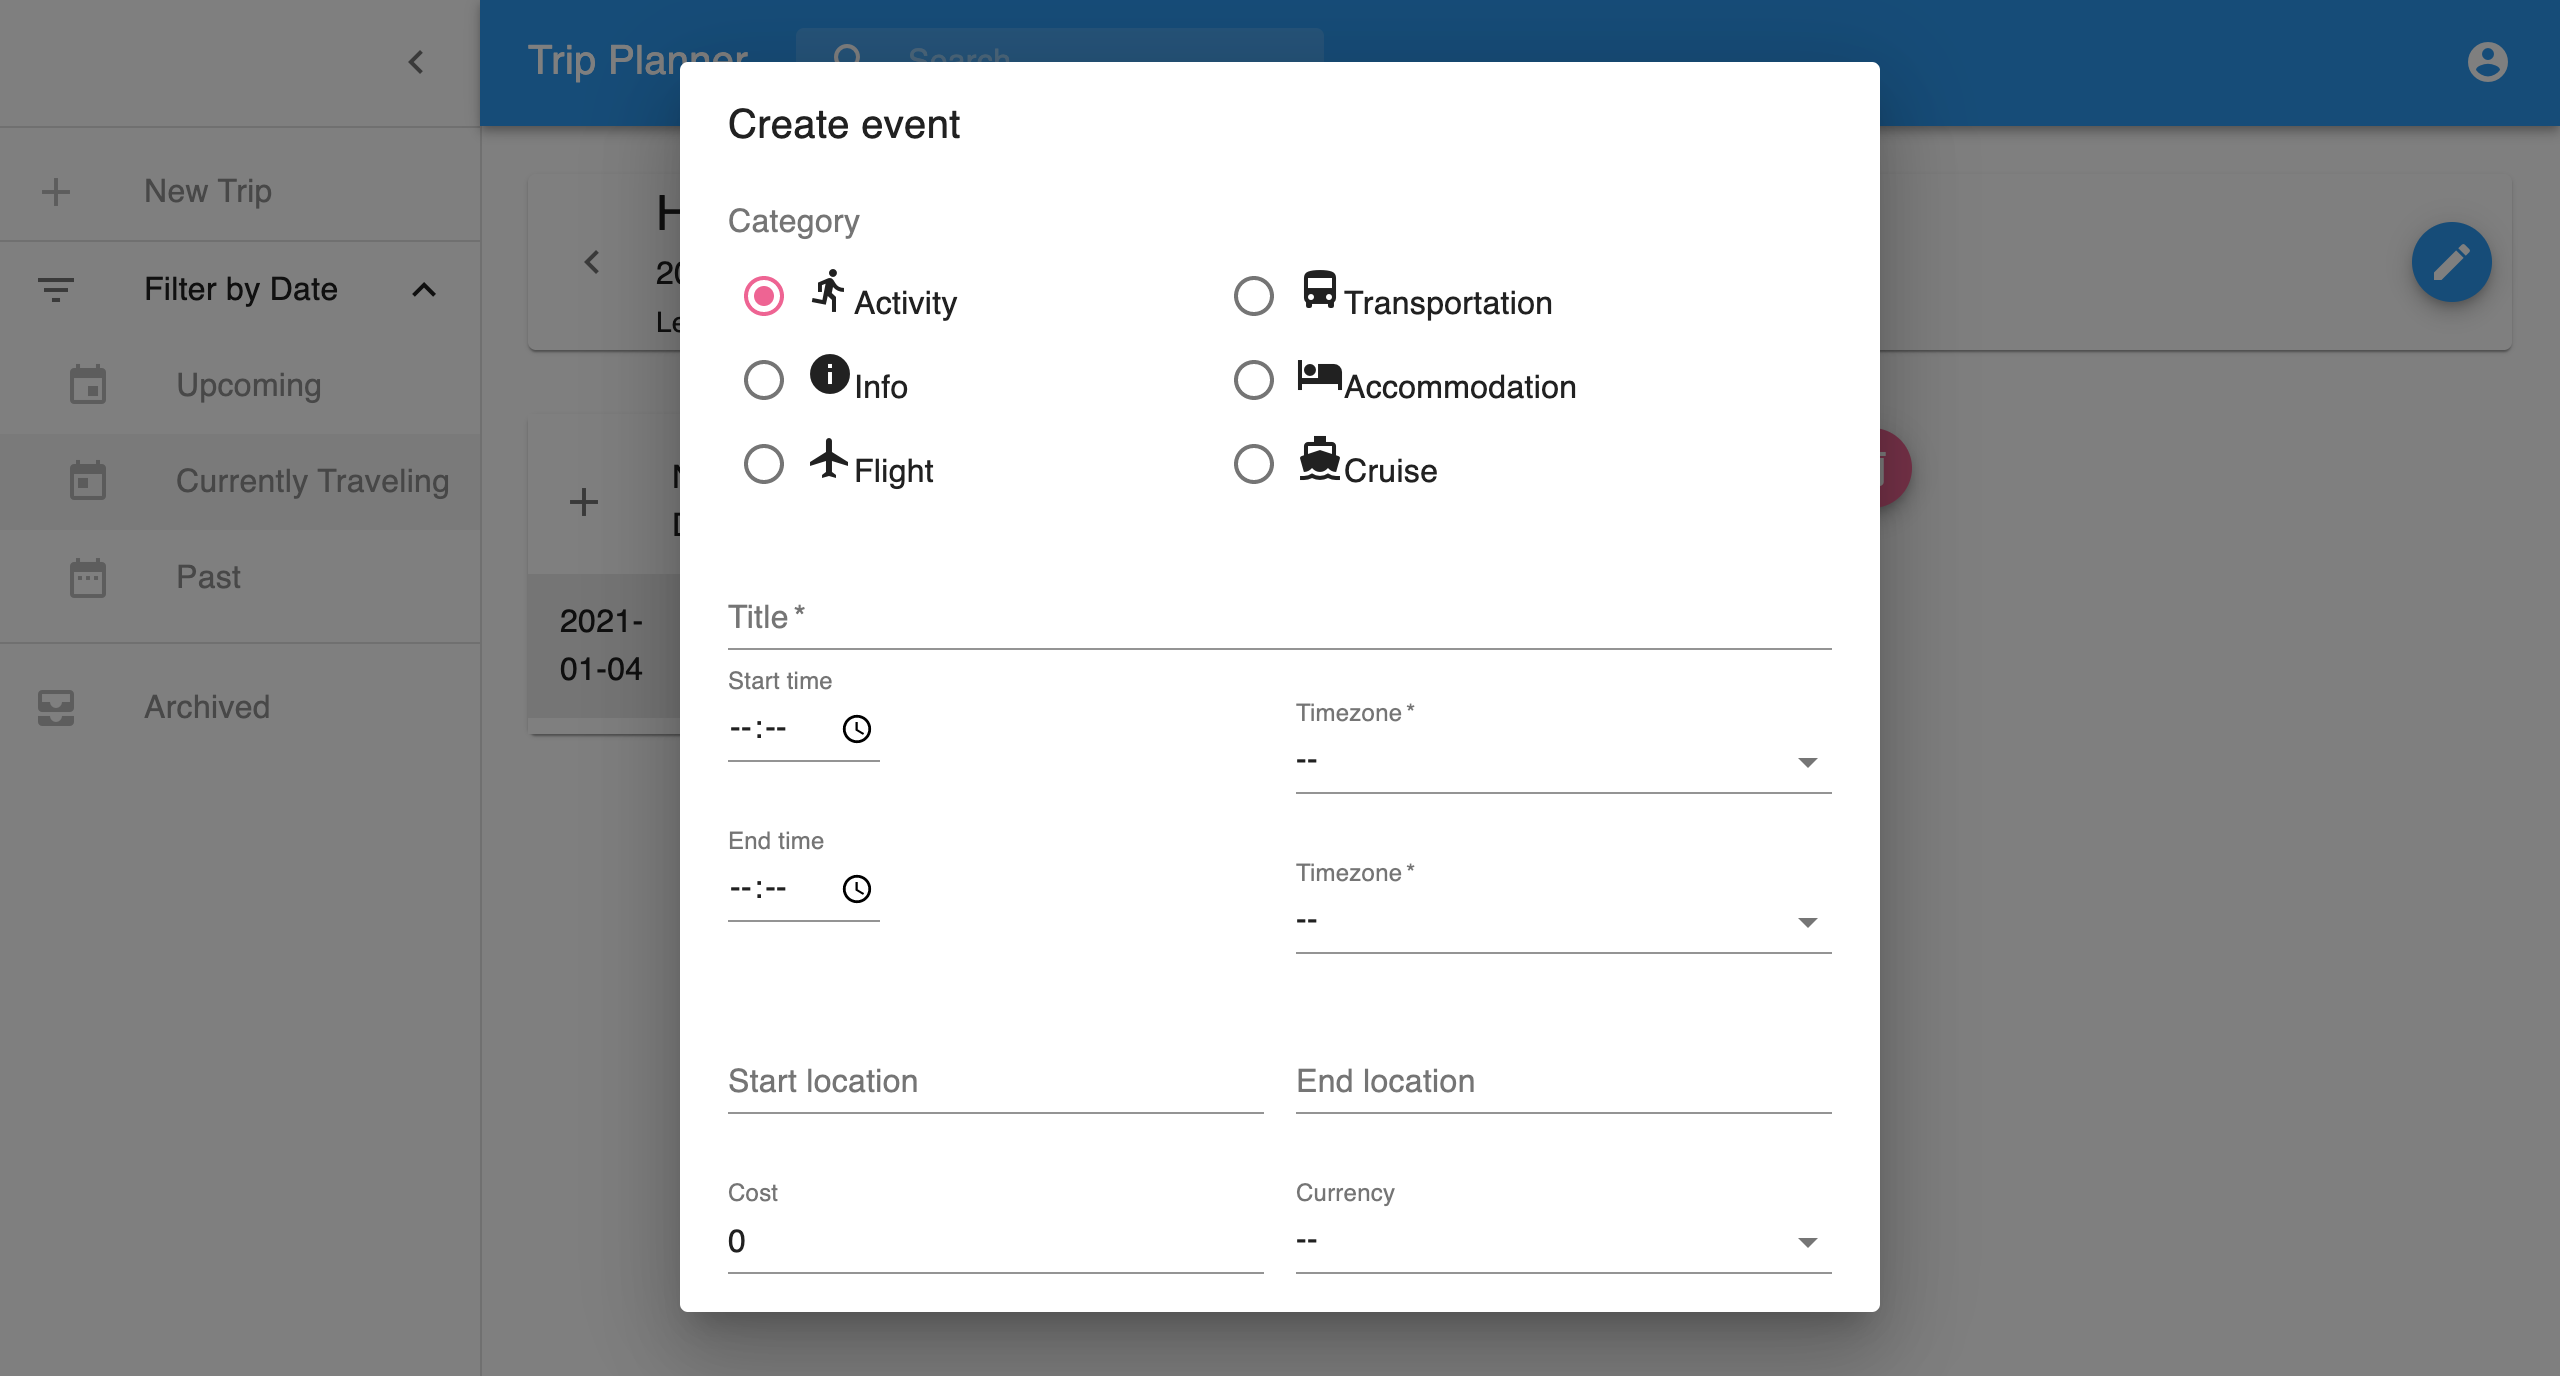
\includegraphics[width=15cm]{document/image/addActivity.png}
%     \caption{Thêm kế hoạch mới}
%     \label{fig:fig_edit_activity}
% \end{figure}

% Danh sách các hoạt động trong ngày giúp người dùng chủ động hơn về thời gian cho chuyến đi \\

% \begin{figure}[H]
%     \centering
%     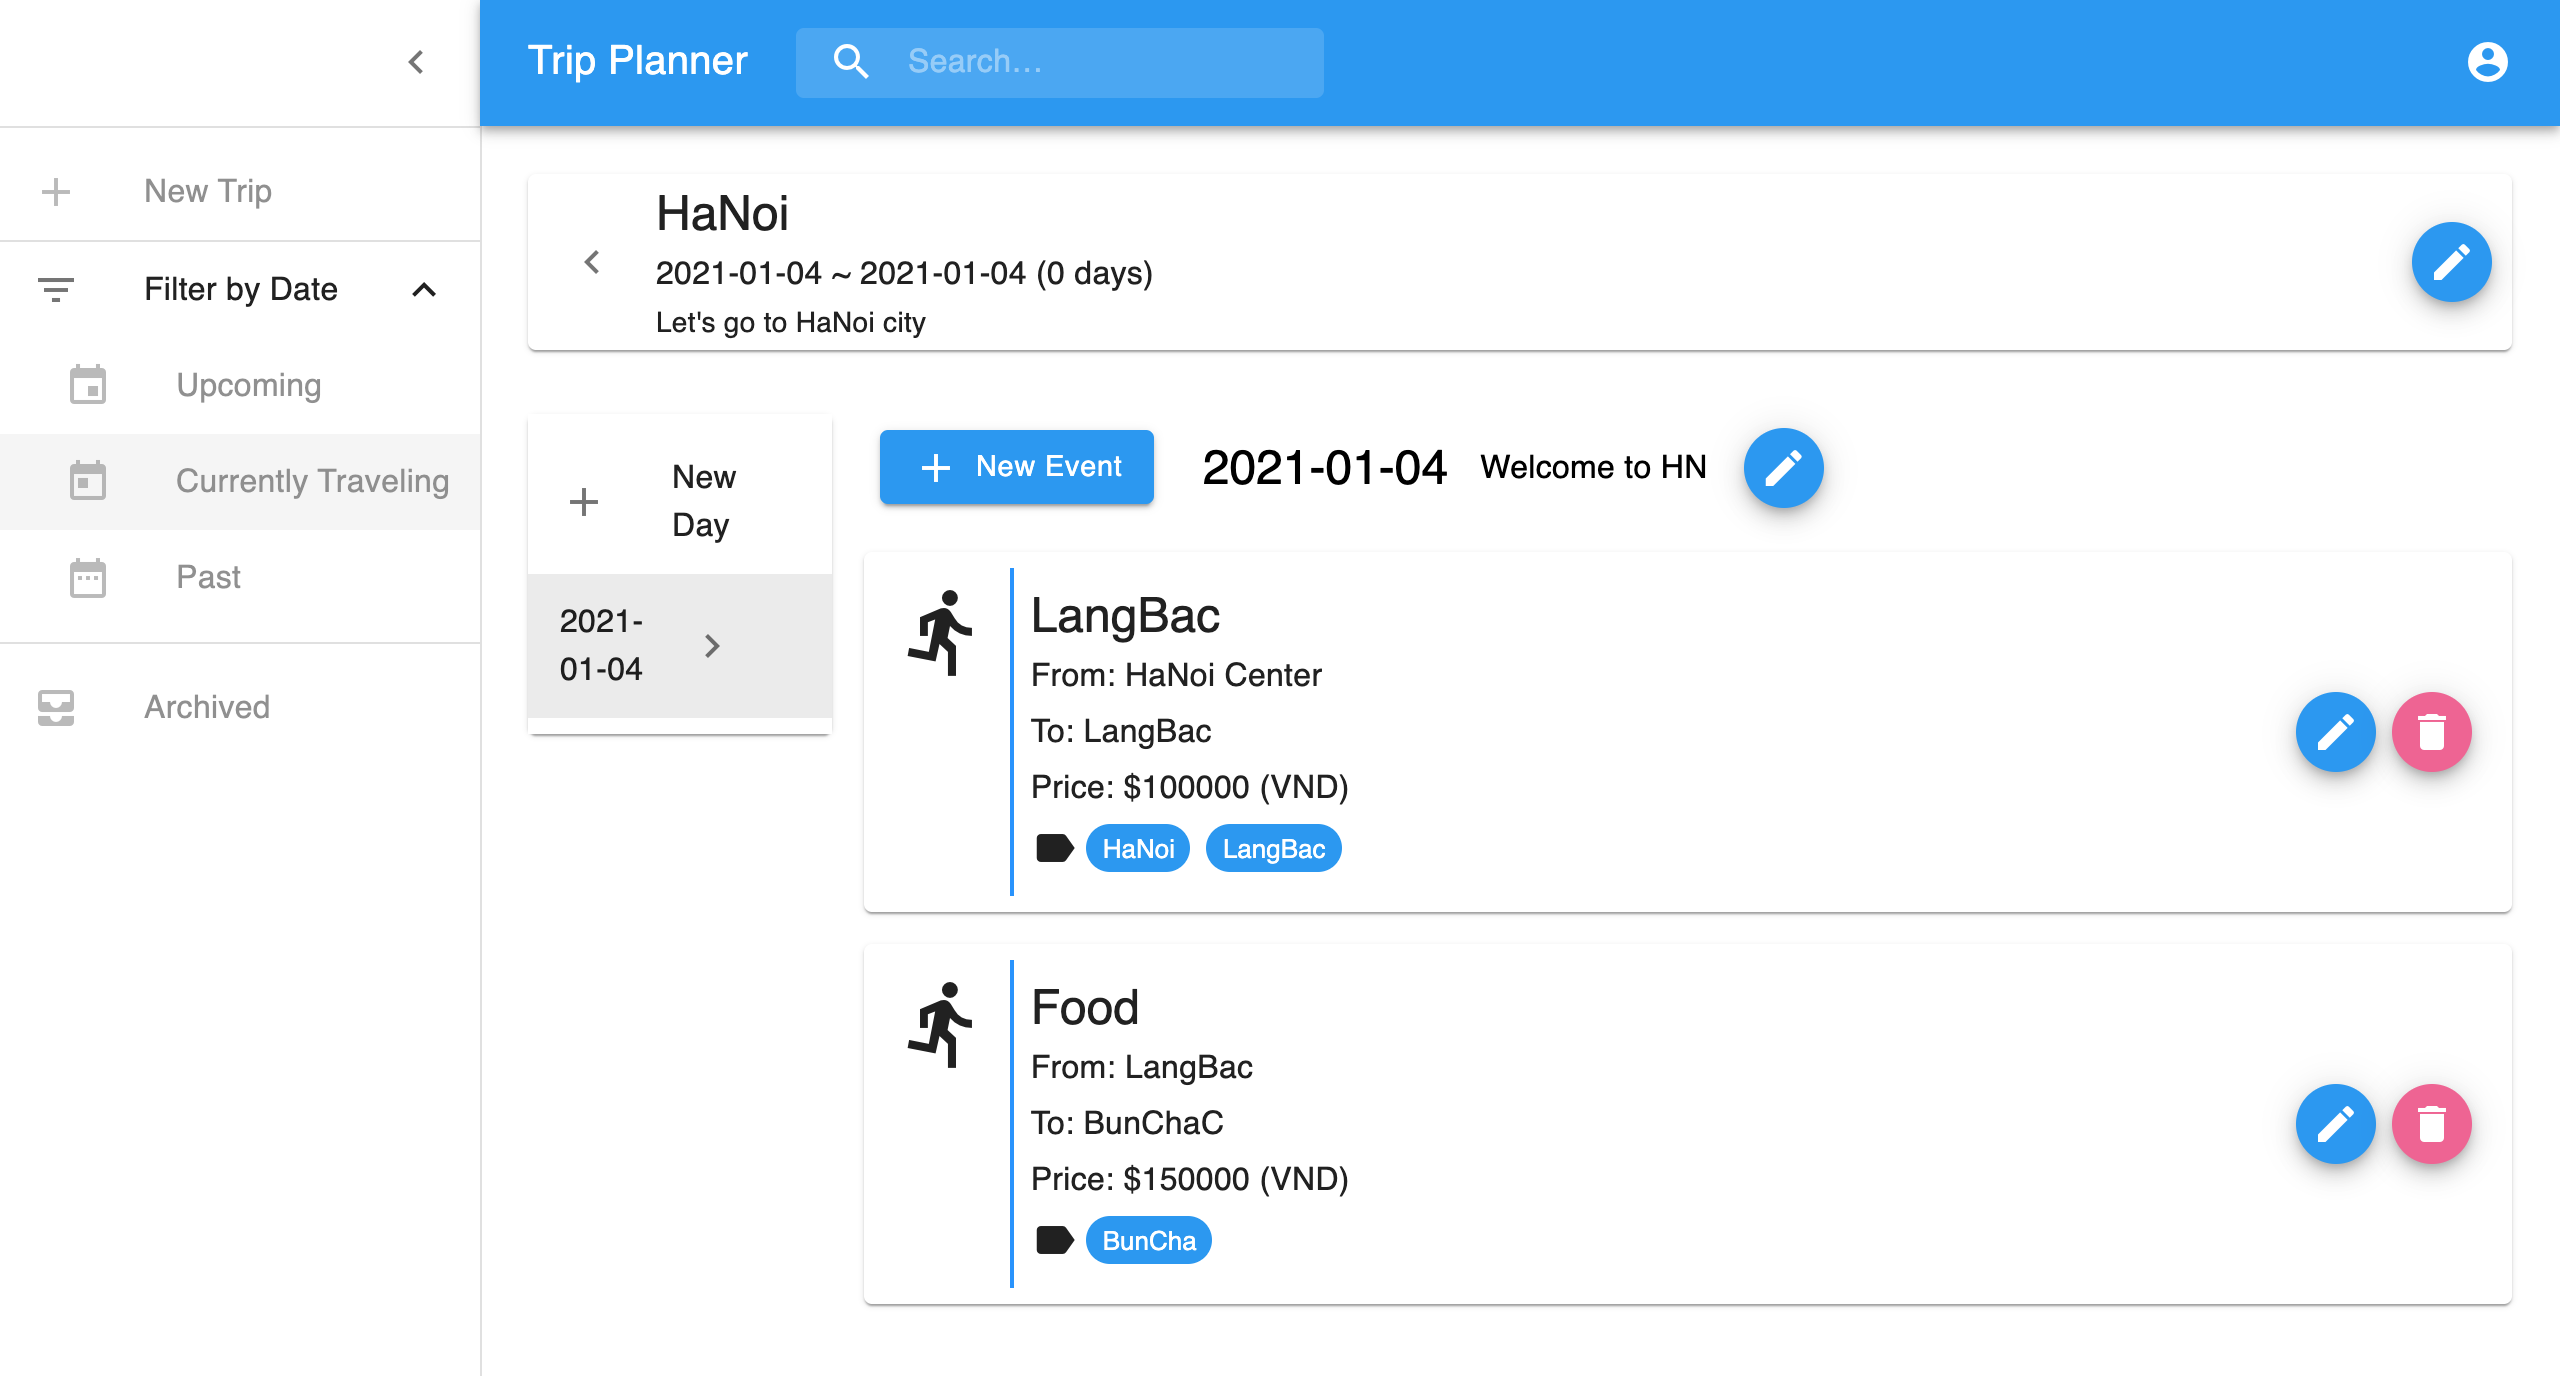
\includegraphics[width=15cm]{document/image/listActivity.png}
%     \caption{Danh sách hoạt động trong ngày}
%     \label{fig:fig_list_activity}
% \end{figure}


% \subsubsection{Chức năng: Quản lý}
% \begin{center}
%   \captionsetup{type=figure}
%   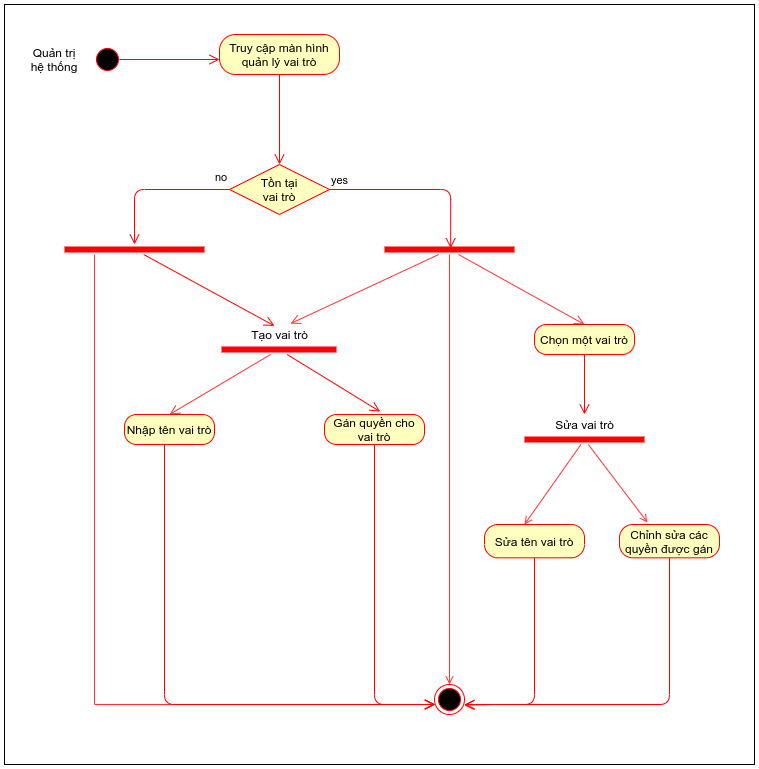
\includegraphics[width=15cm]{image/addRole.png}
%   \captionof{figure}{Lược đồ Activity quản lý vai trò hệ thống}
% \end{center}

% Hệ thống tồn tại cơ chế quản lý vai trò động. Mỗi vai trò được gán với các quyền truy cập. Quản trị viên có thể chỉnh sửa quyền của các vai trò một cách dễ dàng.\\
% \begin{center}
%   \captionsetup{type=figure}
%   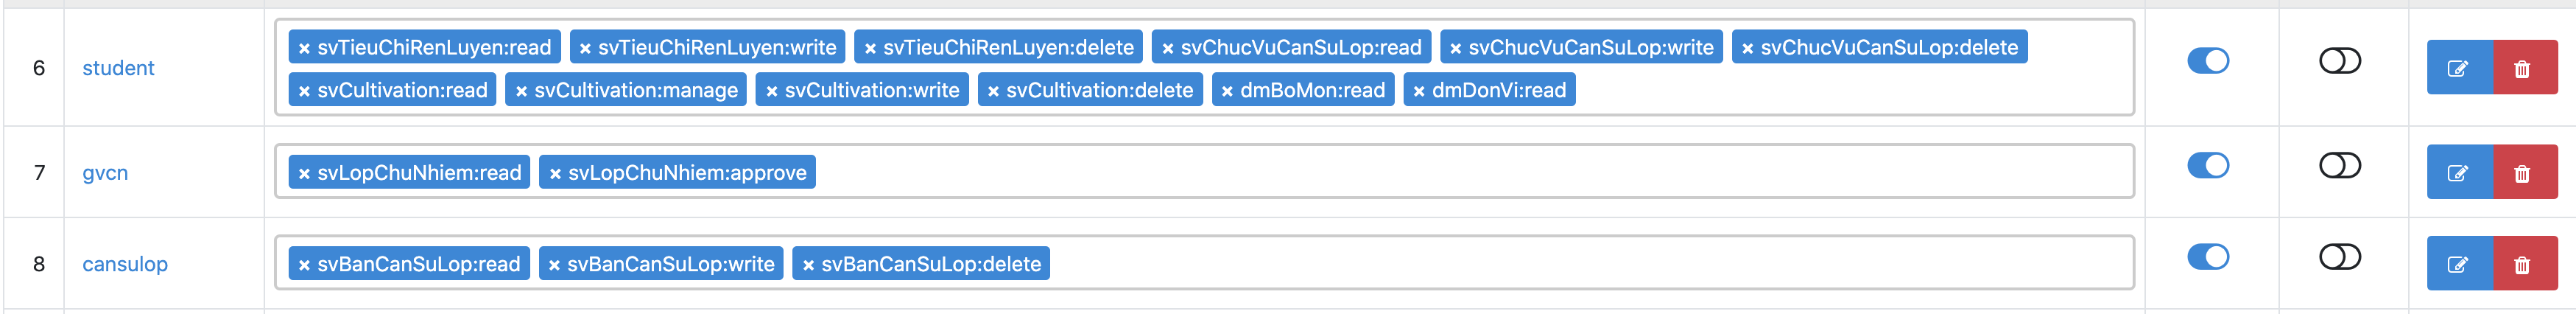
\includegraphics[width=15cm]{image/allrole.png}
%   \captionof{figure}{Danh sách vai trò có trong hệ thống hiện tại}
% \end{center}
% \subsection{Đối tượng: Cán bộ, công nhân viên của nhà trường}
% \subsubsection{Chức năng: Quản lý thông tin}
% \begin{center}
%   \captionsetup{type=figure}
%   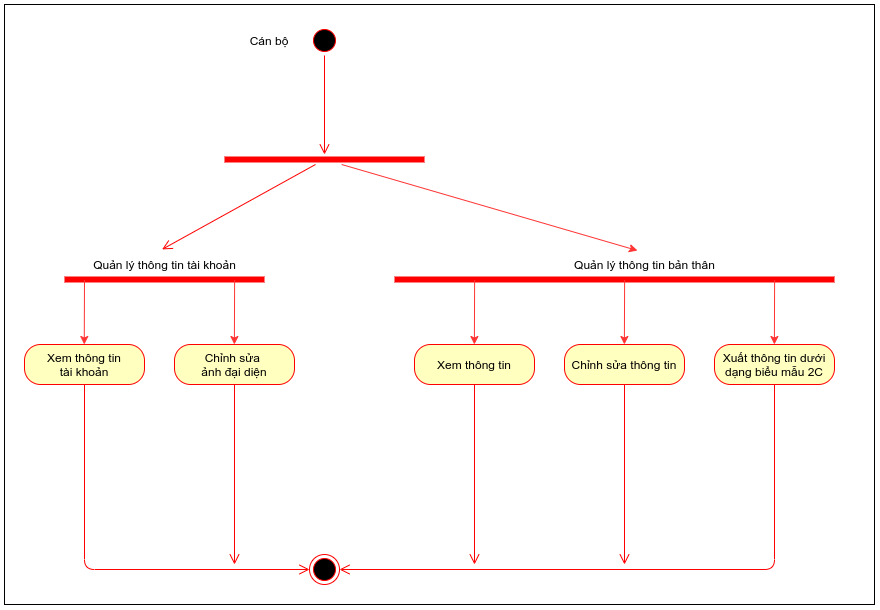
\includegraphics[width=15cm]{image/activityQLThongTin.png}
%   \captionof{figure}{Lược đồ Activity cho chức năng quản lý thông tin cho cán bộ}
% \end{center}

\section{Thiết kế UI Front-end hệ thống}

     Chính vì là hệ thống Website du lịch hỗ trợ người dùng tạo chi tiết chuyến đi nên Front-end là phần được nhóm em tập trung phát triển nhất.UI của hệ thống được nghiên cứu và thiết kế sao cho thân thiện và gây ấn tượng mạnh nhất với người dùng có thể.
     Về màu sắc và Logo cũng do nhóm tự thiết kế. Về UI của hệ thống đã được thiết kế như sau: 
     
     Chi tiết xem ở tài liệu đính kèm
     
     
% \subsection{Page Home}
% \begin{center}
%   \captionsetup{type=figure}
%   \includegraphics[width=12cm]{document/image/Web 1920 – 1.png}
%   \captionof{figure}{UI trang chủ.}
% \end{center}
% \clearpage
% \subsection{Page đăng nhập}
% \begin{center}
% \captionsetup{type=figure}
%   \includegraphics[width=12cm]{document/image/Web 1920 – 2.png}
%   \captionof{figure}{UI Trang đăng nhập.}
% \end{center}

% \subsection{Page List Bài Review}
% \begin{center}
% \captionsetup{type=figure}
%   \includegraphics[width=12cm]{document/image/Web 1920 – 3.png}
%   \captionof{figure}{UI Trang list bài review.}
% \end{center}

% \subsection{Page Bài Review}
% \begin{center}
% \captionsetup{type=figure}
%   \includegraphics[width=12cm]{document/image/Web 1920 – 4.png}
%   \captionof{figure}{UI bài review.}
% \end{center}


% \subsection{Page List Plan}
% \begin{center}
% \captionsetup{type=figure}
%   \includegraphics[width=12cm]{document/image/Web 1920 – 6.png}
%   \captionof{figure}{UI list Plan.}
% \end{center}
% \begin{center}
%   \captionsetup{type=figure}
%   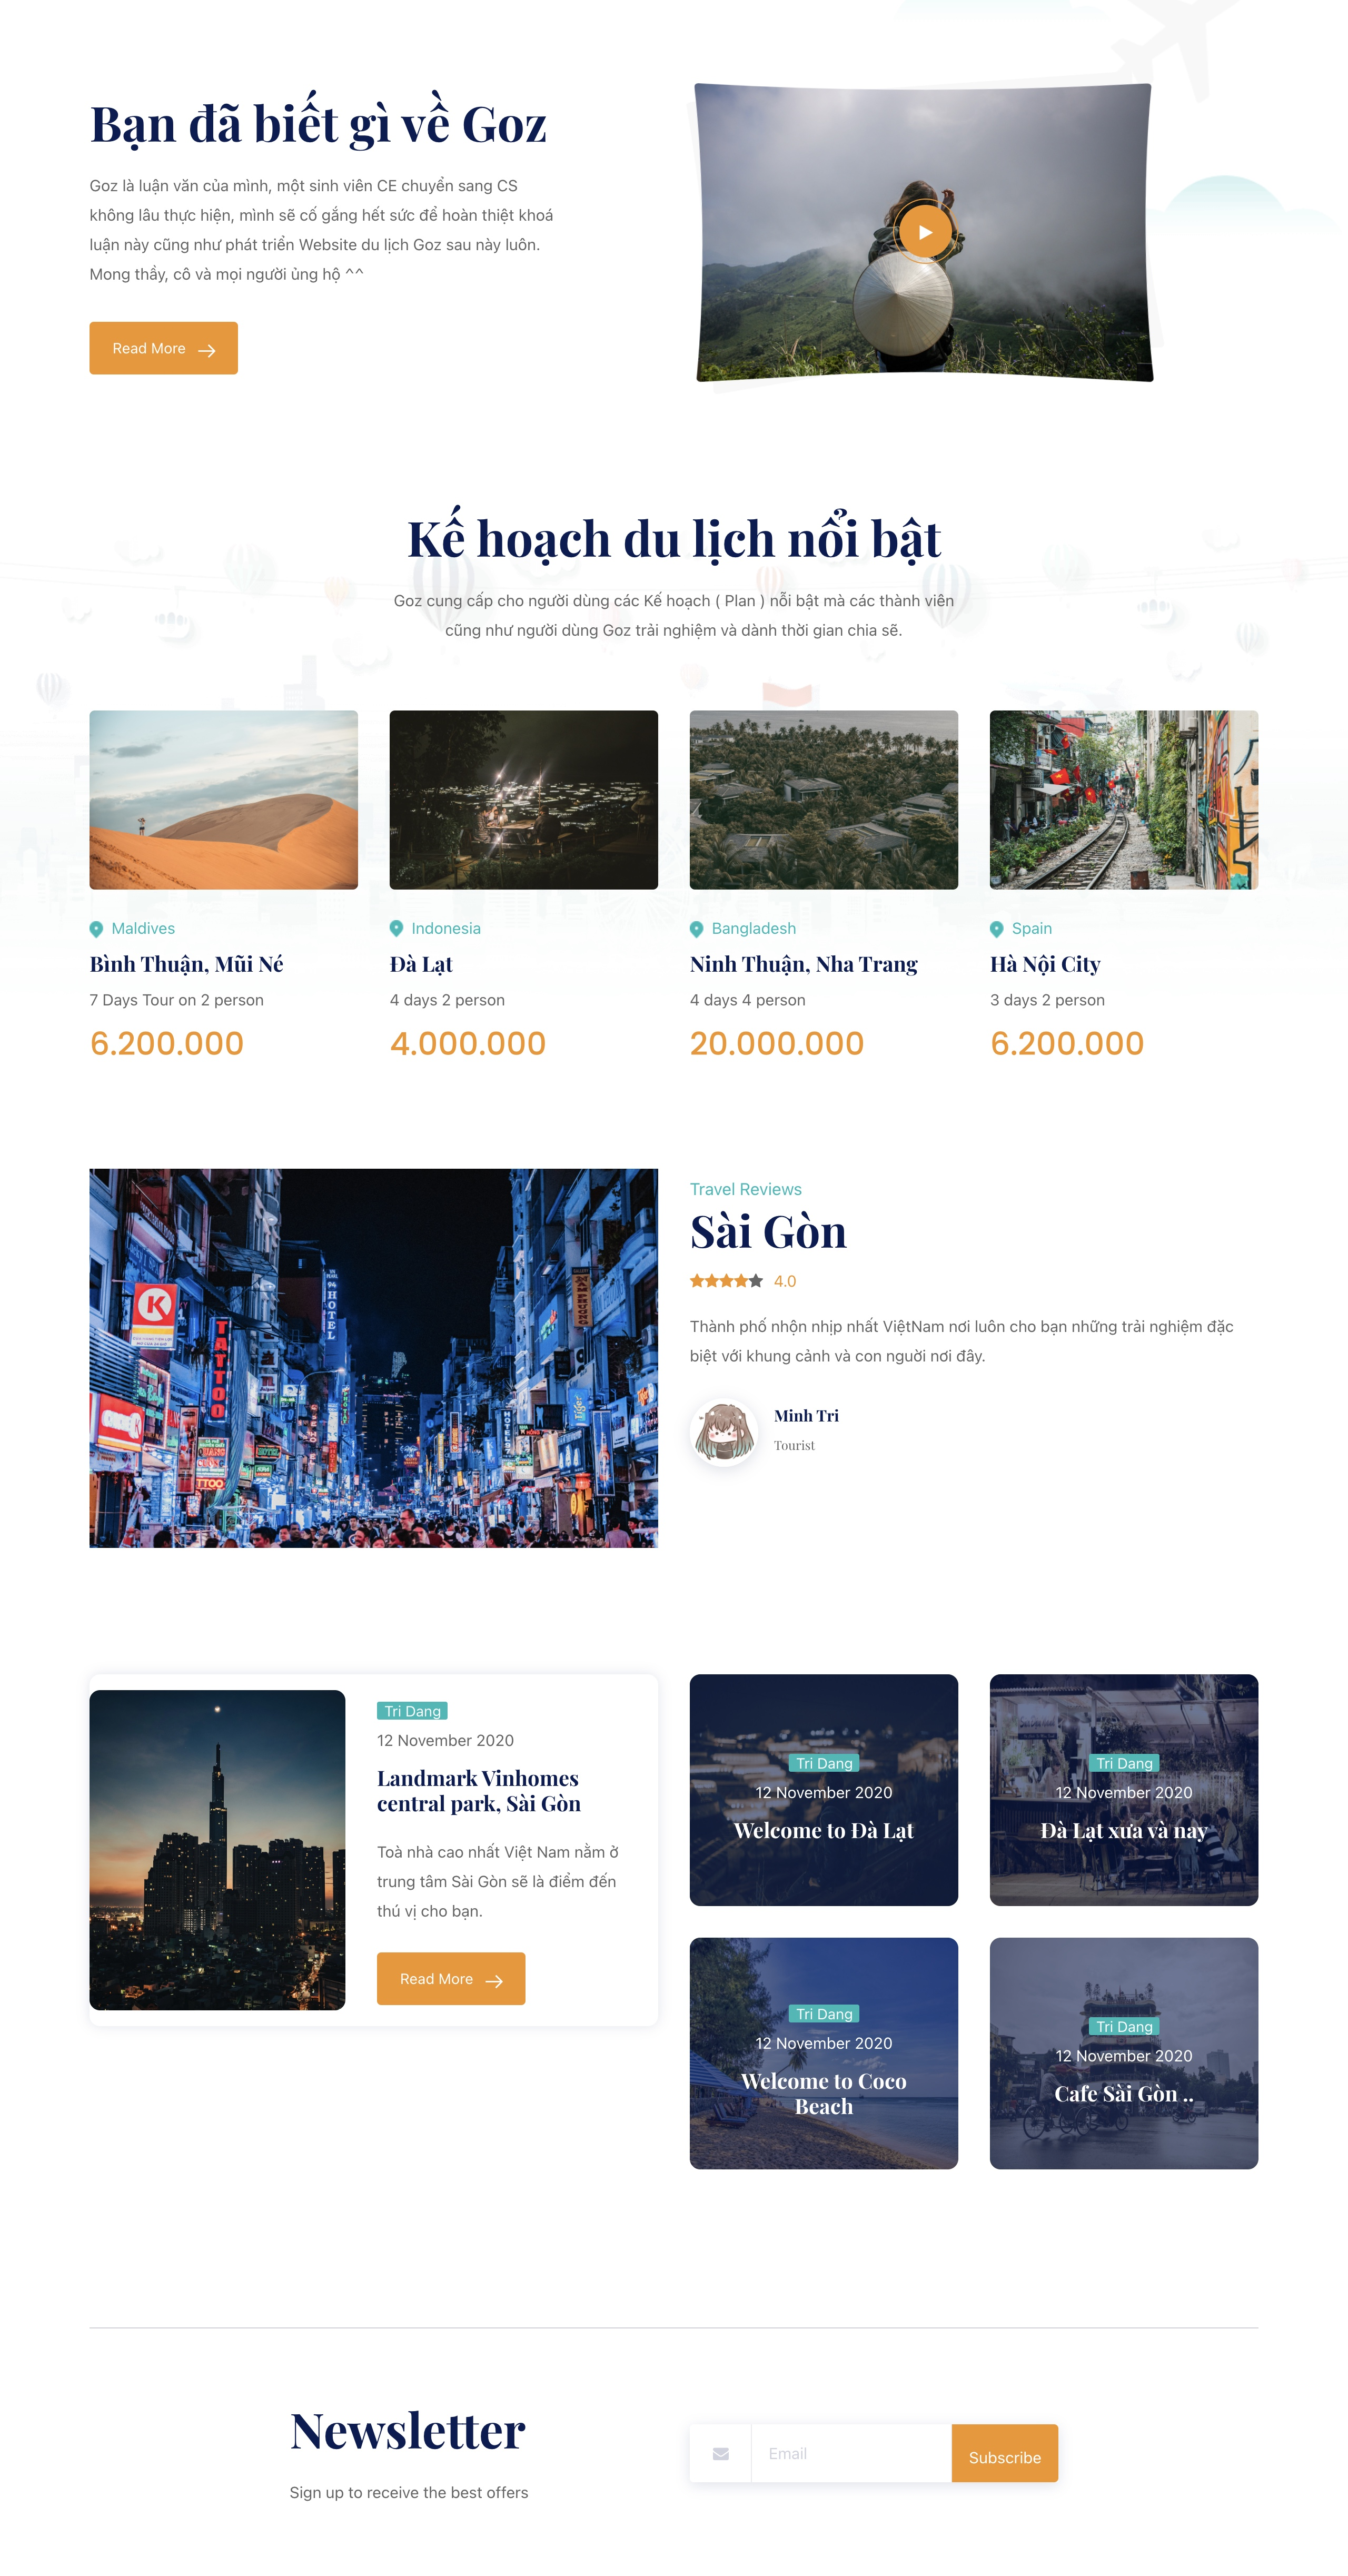
\includegraphics[width=12cm]{document/image/Home4.png}
%   \captionof{figure}{UI trang chủ.}
% \end{center}






%%%%%%%%%%%%%%%%%%%%%%%%%%%%%%%%%%%%%%%%%%%%%%%%%%%%%%%%
\chapter{\textbf{HIỆN THỰC HỆ THỐNG}}

\section{Quản lí mã nguồn}
\subsection{Cấu trúc cây thư mục}
Việc cần làm đầu tiên và quan trọng nhất là tổ chức files và các thư mục. Với một thiết kế tốt thì khi làm việc chung giữa nhiều người sẽ ít bị đụng độ. Nhóm lựa chọn cách chia mỗi thành phần của trang ra từng module tách biệt với nhau, thuận lợi cho việc mở rộng và bảo trì, bảo dưỡng.

Dựa vào kiến trúc hệ thống mà nhóm đã thiết kế ở trên, nhóm đã thiết kế cấu trúc mã nguồn như sau:
\begin{center}
  \captionsetup{type=figure}
  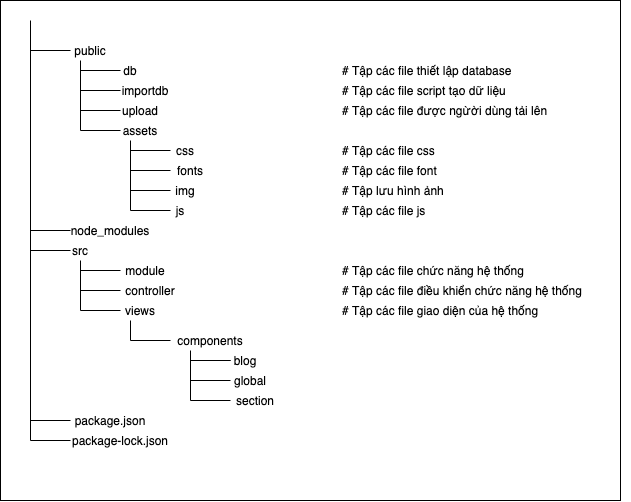
\includegraphics[width=15cm]{document/image/cauTrucThuMuc.png}
  \captionof{figure}{Cây thư mục của hệ thống}
\end{center}
\clearpage
% Nhóm chia các chức năng vào từng module riêng, các module được thiết kế thống nhất theo mô hình MVC kết hợp với Redux. 

% Cách chia module này thuận lợi cho phân chia công việc, tránh đụng độ trong phát triển hệ thống, dễ dàng thêm các module mới trong quá trình mở rộng, giúp cho việc tìm và sửa lỗi trong quá trình bảo trì trở nên đơn giản hơn.
% \begin{figure}[H]
%     \centering
%     \begin{subfigure}[b]{0.4\linewidth}
%         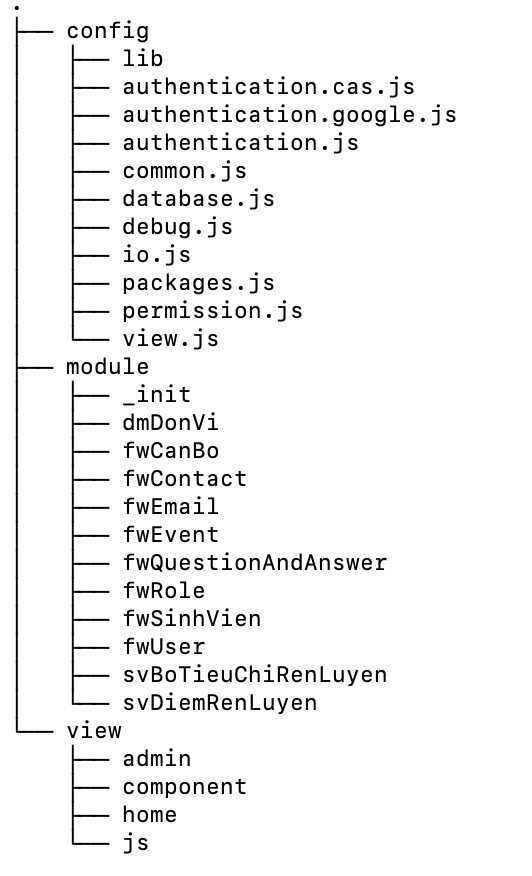
\includegraphics[width=\linewidth]{image/module.png}
%         \caption{Thư mục module}
%     \end{subfigure}
%     \begin{subfigure}[b]{0.4\linewidth}
%         \includegraphics[width=\linewidth]{image/moduleDetail.png}
%         \caption{Chi tiết từng module}
%     \end{subfigure}
%     \caption{Thư mục module của hệ thống}
% \end{figure}
% \clearpage
\subsection{Git}
\begin{center}
  \captionsetup{type=figure}
  \includegraphics[width=15cm]{document/image/AAEAAQAAAAAAAAdxAAAAJDdlNTkxZDk0LTJlNmItNDc1NS1hODdiLTQwZTZiZDdmN2Y0Ng.png}
  \captionof{figure}{Git}
\end{center}

Git là hệ thống quản lý phiên bản phân tán (Distributed Version Control System).\par 
Git hỗ trợ quản lý code và các phiên bản thay đổi của kho chứa mã nguồn (repository), chúng ta có thể thay đổi mã nguồn bằng cách commit và push lên hệ thống này. Git mạnh hơn những hệ thống quản lý mã nguồn khác ở chỗ Git có hỗ trợ cho việc phân nhánh, tạo label, điều này hỗ trợ rất tốt cho việc làm teamwork, chia task cho các thành viên thành những nhánh khác nhau, tạo PR(pull request) trước khi merge vào nhánh chính.\par

\textbf{Vì sao cần sử dụng Git?}
\begin{itemize}
    \item Git dễ sử dụng, an toàn và hiệu quả.
    \item Có thể giúp làm việc nhóm hiệu quả hơn thông qua việc phân nhánh (branch).
    \item Dễ dàng hơn cho việc deployment.
    \item Có thể làm việc bất cứ đâu, bất cứ máy nào, chỉ cần clone mã nguồn hoặc một nhánh nào đó của mã nguồn để làm việc.
\end{itemize}

\subsection{Git Hub}
\begin{center}
  \captionsetup{type=figure}
  \includegraphics[width=15cm]{document/image/github.png}
  \captionof{figure}{Github}
\end{center}

Github là một dịch vụ máy chủ repository công cộng. Mỗi người có thể đăng kí tài khoản để quản lý mã nguồn (repository) riêng của mình. Github hỗ trợ tạo repository ở trạng thái công cộng (public) hoặc chỉ riêng mình người sử dụng (private).\par 
Đường dẫn mã nguồn của dự án:

\href{https://github.com/tri721305/luanvan2020}{Du Lịch Goz}
\clearpage
\section{Giao diện người dùng}
Dựa vào thiết kế UI đã thiết kế nhóm đã tiến hành hiện thực giao hiện người dùng như sau: 
\subsection{Giao diện trang chủ}
\begin{center}
  \includegraphics[width=15cm]{document/image/Home1.png}
\end{center}
\begin{center}
  \includegraphics[width=15cm]{document/image/Home2.png}
\end{center}
\clearpage
\begin{center}
  \captionsetup{type=figure}
  \includegraphics[width=15cm]{document/image/home5.png}
  \captionof{figure}{Trang chủ}
\end{center}


\subsection{Giao diện đăng nhập}
\begin{center}
  \captionsetup{type=figure}
  \includegraphics[width=15cm]{document/image/loginPage.png}
  \captionof{figure}{Trang đăng nhập}
\end{center}

\subsection{Giao diện danh sách bài Review}
\begin{center}
    \includegraphics[width=15cm]{document/image/dsBaiReview.png}
\end{center}
\clearpage
\begin{center}
  \captionsetup{type=figure}
  \includegraphics[width=15cm]{document/image/dsBaiReview2.png}
  \captionof{figure}{Trang danh sách bài Review}
\end{center}
\clearpage

\subsection{Giao diện bài Review}
\begin{center}
    \includegraphics[width=15cm]{document/image/baireview1.png}
\end{center}
\clearpage
\begin{center}
    \includegraphics[width=15cm]{document/image/baireview2.png}
\end{center}
\clearpage
\begin{center}
  \captionsetup{type=figure}
  \includegraphics[width=15cm]{document/image/baireview3.png}
  \captionof{figure}{Bài Review}
\end{center}
\clearpage

\subsection{Giao diện blog giới thiệu điểm đến}
\begin{center}
    \includegraphics[width=15cm]{document/image/dsBlog.png}
\end{center}
\begin{center}
  \captionsetup{type=figure}
  \includegraphics[width=15cm]{document/image/dsBlog2.png}
  \captionof{figure}{Danh sách Blog}
\end{center}
\clearpage

\subsection{Giao diện bài blog}
\begin{center}
    \includegraphics[width=15cm]{document/image/blogdetail1.png}
\end{center}
\clearpage
\begin{center}
    \includegraphics[width=15cm]{document/image/blogdetail2.png}
\end{center}
\clearpage
\begin{center}
  \captionsetup{type=figure}
  \includegraphics[width=15cm]{document/image/blogdetail3.png}
  \captionof{figure}{Giao diện bài Blog}
\end{center}
\clearpage

\subsection{Giao diện thông tin người dùng}
\begin{center}
    \captionsetup{type=figure}  
    \includegraphics[width=15cm]{document/image/in4User1.png}
    \captionof{figure}{Giao diện thông tin người dùng}
\end{center}


\subsection{Giao diện danh sách kế hoạch}
\begin{center}
    \captionsetup{type=figure}  
    \includegraphics[width=15cm]{document/image/listplans.png}
    \captionof{figure}{Danh sách kế hoạch}
\end{center}

\begin{center}
    \captionsetup{type=figure}  
    \includegraphics[width=15cm]{document/image/plan.png}
    \captionof{figure}{Plan}
\end{center}
\clearpage
\begin{center}
    \captionsetup{type=figure}  
    \includegraphics[width=15cm]{document/image/addhoatdong.png}
    \captionof{figure}{Plan thêm hoạt động cho kế hoạch}
\end{center}

\clearpage
\section{Triển khai dự án thực tế}
\subsection{Tìm hiểu heroku}
\begin{center}
    \captionsetup{type=figure}  
    \includegraphics[width=15cm]{document/image/heroku.png}
    \captionof{figure}{Heroku}
\end{center}

Heroku là một nền tảng đám mây để xây dựng và triển khai ứng dụng. Cung cấp một cách đơn giản cho các nhà phát triển có thể tập trung vào việc phát triển sản phẩm mà không cần quan tâm hay có hiểu biết quá tường tận về máy chủ và phần cứng.
Heroku chạy các ứng dụng trong dynos, có hỗ trợ gói miễn phí và các addons hỗ trợ rất hữu ích. Heroku hỗ trợ nhiều ngôn ngữ lập trình như:

\begin{itemize}
    \item \textbf{Nodejs}
    \item Ruby
    \item Python
    \item PHP
    \item Java
    \item ...
\end{itemize}
Thêm vào đó, Heroku còn hỗ trợ SSL miễn phí, cung cấp database, hỗ trợ làm việc theo team và cung cấp liên kết với Git hiệu quả và đơn giản.

\subsection{Triển khai dự án lên Heroku}
Với mong muốn đưa vào thử nghiệm thực tế, dự án đã được deploy lên Heroku theo đường dẫn sau: 
\href{https://travelgoz.com/vi/}{Du lịch Goz}







% Người dùng sử dụng tài khoản trường Đại học Bách Khoa của mình để đăng nhập. Sau khi đăng nhập thành công, hệ thống xác thực tập trung (SSO) sẽ trả về cho hệ thống email tài khoản của người dùng. Lúc này hệ thống sẽ kiểm tra, email nhận được đã được quản trị viên thêm vào hệ thống thì người dùng sẽ đăng nhập được vào hệ thống và thực hiện các chức năng với vai trò của mình.\\

% Đối với từng vai trò, sau khi đăng nhập vào hệ thống sẽ có các menu như sau:
% \begin{center}
%   \captionsetup{type=figure}
%   \includegraphics[width=15cm]{image/canbo.png}
%   \captionof{figure}{Menu của người dùng là CBCNV của trường}
% \end{center}
% \begin{center}
%   \captionsetup{type=figure}
%   \includegraphics[width=15cm]{image/eventManager.png}
%   \captionof{figure}{Menu của người dùng là quản lý sự kiện}
% \end{center}
% \begin{center}
%   \captionsetup{type=figure}
%   \includegraphics[width=15cm]{image/diemRenLuyenAdmin.png}
%   \captionof{figure}{Menu tất cả các vai trò về điểm rèn luyện}
% \end{center}
% \clearpage
% \section{Các trang tính năng quản lý cụ thể}
% \subsection{Quản lý bài viết sự kiện} \label{news_management}
% \subsubsection{Quản lý danh mục} \label{category_management}
% Quản trị viên có thể \textbf{thêm, sửa, xoá, thay đổi thứ tự} các danh mục thuộc loại sự kiện. Các danh mục này sẽ được dùng trong phần \textbf{tạo/chỉnh sửa} một sự kiện cụ thể (hình \ref{fig:category_news}).
% \begin{figure}[H]
%     \centering
%     \begin{subfigure}[b]{0.6\linewidth}
%         \includegraphics[width=\linewidth]{image/danh_sach_category.png}
%         \caption{Danh sách danh mục của sự kiện}
%     \end{subfigure}
%     \begin{subfigure}[b]{0.3\linewidth}
%         \includegraphics[width=\linewidth]{image/chinh_sua_category.png}
%         \caption{Chọn tên thành phần}
%     \end{subfigure}
%     \caption{Cấu hình danh mục cho sự kiện}
%     \label{fig:category_news}
% \end{figure}
% \subsubsection{Chỉnh sửa sự kiện}
% Quản trị viên có thể \textbf{tạo mới, chỉnh sửa, xoá} sự kiện. Hình \ref{fig:chinh_sua_news} trình bày giao diện chỉnh sửa sự kiện 
% về \textbf{tiêu đề, kích hoạt, hình ảnh, ngày tháng} của sự kiện. Quản trị viên cũng có thể \textbf{gán các danh mục} cho sự kiện đang chỉnh sửa,
% các danh mục này có được từ việc tạo danh mục sự kiện ở phần \ref{category_management} (hình \ref{fig:gan_danh_muc}).

% \begin{figure}[H]
%     \centering
%     \includegraphics[width=\linewidth]{image/chinh_sua_news.png}
%     \caption{Chỉnh sửa sự kiện: tiêu đề, hình ảnh, thời gian}
%     \label{fig:chinh_sua_news}
% \end{figure}

% \begin{figure}[H]
%     \centering
%     \includegraphics[width=7cm]{image/gan_danh_muc.png}
%     \caption{Gán danh mục cho sự kiện}
%     \label{fig:gan_danh_muc}
% \end{figure}
% \begin{figure}[H]
%     \centering
%     \includegraphics[width=12cm]{image/tom_tat_tin_tuc.png}
%     \caption{Tóm tắt, nội dung của sự kiện}
%     \label{fig:tom_tat_tin_tuc}
% \end{figure}


% Ngoài ra, quản trị viên cũng có thể chỉnh sửa phần \textbf{tóm tắt} cũng như là \textbf{soạn thảo nội dung} của sự kiện (hình \ref{fig:tom_tat_tin_tuc})

% \subsection{Quản lý sự kiện}
% \subsubsection{Năm học xét điểm rèn luyện, người đại diện, số lượng đăng ký, điểm rèn luyện, công tác xã hội, câu hỏi sự kiện}
% \begin{figure}[H]
%  \centering
%     \includegraphics[width=16cm]{image/chinh_sua_event_2.png}
%     \caption{Cấu hình cho sự kiện}
%     \centering
%     \label{fig:chinh_sua_event}
% \end{figure}
% \begin{figure}[H]
%     \centering
%     \includegraphics[width=13cm]{image/cau_hoi_su_kien.png}
%     \caption{Thiết lập câu hỏi cho sự kiện}
%     \label{fig:cau_hoi_su_kien}
% \end{figure}
% Ở phần này, quản trị viên có thể chỉnh sửa một số tính năng khác của sự kiện như:
% \begin{itemize}
%     \item \textbf{Chương trình năm học:} Nếu sự kiện này thuộc một trong các chương trình của năm học nào đó, thì quản trị viên sẽ gán sự kiện đó với
%     chương trình năm học tương ứng. Việc gán sự kiện cho chương trình năm học sẽ giúp cho quản trị viên cũng như hệ thống thực hiện việc \textbf{chấm/quản lý
%     điểm rèn luyện} cho sinh viên.
%     \item \textbf{Tạo câu hỏi cho sự kiện:} sự kiện sẽ có phần đăng ký tham gia sự kiện cho sinh viên, nên công việc tạo form đăng ký là cần thiết. 
%     Mô tả ở hình \ref{fig:cau_hoi_su_kien} sẽ hỗ trợ quản trị viên trong công việc này và kết quả của form được trình bày như hình \ref{fig:home_dang_ky_su_kien}.
%     \begin{figure}[H]
%         \centering
%         \includegraphics[width=10cm]{image/home_dang_ky_su_kien.png}
%         \caption{Giao diện form đăng ký}
%         \label{fig:home_dang_ky_su_kien}
%     \end{figure}
% \end{itemize}
% \subsubsection{Danh sách sinh viên tham gia sự kiện}
% \begin{itemize}
%     \item Quản trị viên cũng có thể xem thông tin câu trả lời của sinh viên tham gia, và có thể xuất ra file excel danh sách tất cả sinh viên kèm theo câu trả lời của từng người (hình \ref{fig:xem_form_chi_tiet}).
%     \begin{figure}[H]
%         \centering
%         \includegraphics[width=15cm]{image/xem_form_chi_tiet.png}
%         \caption{Chi tiết câu trả lời}
%         \label{fig:xem_form_chi_tiet}
%     \end{figure}
%      \item Quản trị viên cũng có thể thêm sinh viên tham gia.
%     \begin{figure}[H]
%         \centering
%         \includegraphics[width=15cm]{image/add_student_join.png}
%         \caption{Thêm sinh viên tham gia}
%         \label{fig:add_student_join}
%     \end{figure}
%     \item Trong những sự kiện quan trọng (ví dụ như là sự kiện "Buổi định hướng phân ngành CSE - 2019") thì sẽ có số lượng sinh viên bắt buộc 
%     tham gia nhất định, trong trường hợp này quản trị viên có thể import danh sách sinh viên tham gia sự kiện thông qua file excel. Sau khi 
%     import thành công, hệ thống sẽ tự động gửi email/thông báo đến từng sinh viên về sự kiện đó (hình \ref{fig:import_ds_sinh_vien}).
%     \begin{figure}[H]
%         \centering
%         \includegraphics[width=10cm]{image/import_ds_sinh_vien.png}
%         \caption{Import danh sách sinh viên}
%         \label{fig:import_ds_sinh_vien}
%     \end{figure}
%     \clearpage
%     \item Quản trị viên cũng có thể điểm danh sinh viên (theo MSSV hoặc tên của sinh viên) tham gia sự kiện (hình \ref{fig:admin_diem_danh}). và xuất danh sách sinh viên bằng excel.
%     \begin{figure}[H]
%         \centering
%         \includegraphics[width=15cm]{image/admin_diem_danh.png}
%         \caption{Điểm danh sinh viên tham dự}
%         \label{fig:admin_diem_danh}
%     \end{figure}
%       \item Quản trị viên có thể xem được  viên (theo MSSV hoặc tên của sinh viên) tham gia sự kiện (hình \ref{fig:admin_diem_danh}). và xuất danh sách sinh viên bằng excel.
%     \begin{figure}[H]
%         \centering
%         \includegraphics[width=15cm]{image/danh_sach_sv_register.png}
%         \caption{Danh sách sinh sinh viên tham dự}
%         \label{fig:danh_sach_sv_register}
%     \end{figure}
% \end{itemize}
% \clearpage
% \subsection{Quản lý bộ tiêu chí}
% Trường Đại học Bách Khoa sẽ có đưa ra một bộ tiêu chí dùng để xét điểm rèn luyện của sinh viên cho cả năm học(theo Thông tư số 16 năm 2015 của Bộ GDĐT). Gồm các tiêu chí và yếu tố rèn luyện với các số điểm cộng trừ cụ thể và giới hạn số lần trong một học kỳ. Mỗi tiêu chí có thể được cộng và trừ nhiều điểm nhưng không được vuợt khung từng tiêu chí và ĐRL không quá 100. 
%  \begin{figure}[H]
%         \centering
%         \includegraphics[width=\linewidth]{image/bo_tieu_chi_chuan.png}
%         \caption{Bộ tiêu chí chuẩn của Trường Đại Học Bách Khoa}
%         \label{fig:bo_tieu_chi_chuan}
%     \end{figure}
%  Có thể chỉnh sửa, thêm mới, kích hoạt hoặc xoá các tiêu chí rèn luyện. Ngoài ra có thể thêm một yếu tố rèn luyện vào một tiêu chí. 
%  \begin{figure}[H]
%         \centering
%         \includegraphics[width=13cm]{image/thao_tac_tieu_chi.png}
%         \caption{Các thao tác với một tiêu chí rèn luyện}
%         \label{fig:thao_tac_bo_tieu_chi}
%     \end{figure}
% \begin{figure}[H]
%     \centering
%     \begin{subfigure}[b]{0.5\linewidth}
%         \includegraphics[width=\linewidth]{image/chinh_sua_tieu_chi.png}
%         \caption{Chỉnh sửa một tiêu chí rèn luyện}
%     \end{subfigure}
%     \begin{subfigure}[b]{0.5\linewidth}
%         \includegraphics[width=\linewidth]{image/add_yeu_to.png}
%         \caption{Thêm hoặc bớt các yếu tố}
%     \end{subfigure}
%     \caption{Chỉnh sửa một tiêu chí rèn luyện cụ thể}
% \end{figure}

% Chỉnh sửa, kích hoạt hoặc xoá các yếu tố rèn luyện. 
% \begin{figure}[H]
%     \centering
%     \begin{subfigure}[b]{0.5\linewidth}
%         \includegraphics[width=\linewidth]{image/thao_tac_yeu_to.png}
%         \caption{Thao tác yếu tố rèn luyện}
%     \end{subfigure}
%     \begin{subfigure}[b]{0.5\linewidth}
%         \includegraphics[width=\linewidth]{image/chinh_sua_yeu_to.png}
%         \caption{Chỉnh sửa một yếu tố}
%     \end{subfigure}
%     \caption{Chỉnh sửa một yếu tố rèn luyện cụ thể}
% \end{figure}
% \clearpage
% Các khoa sẽ có quyền được tạo bản sao từ bộ tiêu chí Trường hoặc các Khoa khác. Có thể chỉnh sửa lại sao cho phù hợp với Khoa đó.
% \begin{figure}[H]
%         \centering
%         \includegraphics[width=13cm]{image/clone_tieu_chi.png}
%         \caption{Tạo bản sao một bộ tiêu chí rèn luyện}
%         \label{fig:clone_tieu_chi}
% \end{figure}
% \begin{figure}[H]
%         \centering
%         \includegraphics[width=13cm]{image/bo_tieu_chi_cac_cap.png}
%         \caption{Bộ tiêu chí rèn luyện các cấp}
%         \label{fig:bo_tieu_chi_cac_cap}
% \end{figure}

 
% \subsection{Quản lý điểm rèn luyện}
% Hệ thống tổ chức quản lý điểm rèn luyện theo từng năm học. Quản trị viên có thể \textbf{theo dõi điểm rèn luyện} của tất cả sinh viên trong năm học đó.
% Những sinh viên có số điểm rèn luyện khác nhau sẽ hiển thị với những nền màu khác nhau. Ngoài ra, quản trị viên có thể xuất điểm rèn 
% luyện của năm học đó với tất cả sinh viên kèm các sự kiện mà sinh viên đã tham gia, quản trị viên còn có thể thực hiện thao tác \textbf{Cập 
% nhật lại điểm rèn luyện} nếu muốn (Chức năng này hệ thống đã lên lịch và cứ mỗi cuối tuần sẽ được tự động cập nhật lại).

% Ngoài ra mỗi cuối năm học sinh viên thực hiện chấm phiếu điểm rèn luyện. Phiếu chấm điểm rèn luyện được dựa trên những yếu tố rèn luyện(đi kèm minh chứng) dựa trên bộ tiêu chí rèn luyện chuẩn của \textbf{Trường Đại Học Bách Khoa}. Sau khi chấm sinh viên được thành phần ban cán sự lớp thực hiện việc duyệt/từ chối những yếu tố mà sinh viên chấm dựa trên những minh chứng có hợp lý hay không. Tương tự sau khi được ban cán sự lớp thông qua sẽ được giáo viên chủ nhiệm duyệt lại một lần nữa trước khi nộp về cho Khoa.

% Khoa sẽ là nơi tổng hợp điểm rèn luyện sinh viên cuối cùng và tiếp nhận phản hồi của sinh viên trước khi gửi kết quả điểm rèn luyện năm học đó về Trường.
% \subsubsection{Cấu hình điểm rèn luyện}
% \begin{itemize}
%     \item Quản trị viên sẽ thực hiện việc cấu hình điểm rèn luyện các email cần thiết.(hình \ref{fig:setting_drl}).
%     \begin{figure}[H]
%         \centering
%         \includegraphics[width=15cm]{image/setting_drl.png}
%         \caption{Cấu hình điểm rèn luyện}
%         \label{fig:setting_drl}
%     \end{figure}

% \item Quản trị viên có thể tiếp nhận phản hồi từ phía sinh viên về tình hình điểm rèn luyện hiện tại của họ, quản trị viên xem xét phản hồi và chỉnh sửa lại điểm rèn luyện cho sinh viên đó nếu cần thiết.
% \clearpage
% \begin{figure}[H]
%     \centering
%     \includegraphics[width=10cm]{image/phan_hoi_drl.png}
%     \caption{Phản hồi điểm rèn luyện từ sinh viên}
%     \label{fig:phan_hoi_drl}
% \end{figure}
% \begin{figure}[H]
%     \centering
%     \includegraphics[width=10cm]{image/chitiet_phanhoi_drl.png}
%     \caption{Nội dung phản hồi điểm rèn luyện từ sinh viên}
%     \label{fig:chitiet_phanhoi_drl}
% \end{figure}
% \item Quản trị viên có thể thêm, xoá và chỉnh sửa các chức vụ ban cán sự lớp để phục vụ cho mục đích sắp xếp lớp trong một Khoa.
% \begin{figure}[H]
%     \centering
%     \includegraphics[width=15cm]{image/chuc_vu_cs.png}
%     \caption{Thao tác với chức vụ các sự lớp}
%     \label{fig:chuc_vu_cs}
% \end{figure}
% \end{itemize}
% \subsection{Vai trò duyệt điểm rèn luyện}
% Sau khi nộp phiếu chấm điểm rèn luyện cần qua hai lần duyệt để đảm bảo tính trung thực, chính xác. Đầu tiên sẽ được duyệt bởi ban cán sự lớp. Sau đó được duyệt bởi giáo viên chủ nhiệm trước khi gửi về Khoa.
% \subsubsection{Ban cán sự lớp}
% Ban cán sự lớp sẽ tổng hợp điểm của các thành viên trong lớp của mình. Gửi email yêu cầu thành viên nộp phiếu chấm rèn luyện(nếu chưa nộp). Khoá phiếu chấm nếu quá hạn mà sinh viên chưa nộp.
% \begin{figure}[H]
%     \centering
%     \includegraphics[width=\linewidth]{image/can_su_cham.png}
%     \caption{Giao diện ban cán sự lớp duyệt điểm rèn luyện}
%     \label{fig:can_su_cham}
% \end{figure}
% Chi tiết từng sinh viên. Cán sự có thể chấm lại: thêm, chỉnh sửa yếu tố rèn luyện và để lại phản hồi.
% \begin{figure}[H]
%     \centering
%     \includegraphics[width=\linewidth]{image/detail_sv_cultivation.png}
%     \caption{Chi tiết duyệt phiếu chấm điểm rèn luyện}
%     \label{fig:detail_sv_cultivation}
% \end{figure}
% \begin{figure}[H]
%     \centering
%     \begin{subfigure}[b]{0.5\linewidth}
%         \includegraphics[width=\linewidth]{image/view_minh_chung.png}
%         \caption{Xem minh chứng của một yếu tố}
%     \end{subfigure}
%     \begin{subfigure}[b]{0.5\linewidth}
%         \includegraphics[width=\linewidth]{image/change_diem.png}
%         \caption{Chỉnh sửa điểm và để lại phản hồi}
%     \end{subfigure}
%     \caption{Duyệt phiếu chấm điểm rèn luyện sinh viên}
% \end{figure}
% \subsubsection{Giáo viên chủ nhiệm}

% Giáo viên chủ nhiệm lớp cũng sẽ có vai trò tương tự ban cán sự lớp có thể duyệt và phản hồi điểm rèn luyện sinh viên. Gửi email yêu cầu thành viên nộp phiếu chấm rèn luyện(nếu chưa nộp). Khoá phiếu chấm nếu quá hạn mà sinh viên chưa nộp.

% Ngoài ra còn có thể gán thành phần ban cán sự lớp cho lớp mình chủ nhiệm tại mỗi năm học.
% \begin{figure}[H]
%     \centering
%     \includegraphics[width=\linewidth]{image/gvcn_assign_student.png}
%     \caption{Giao diện gán thành phần ban cán sự cho lớp chủ nhiệm}
%     \label{fig:gvcn_assign_student}
% \end{figure}
% \subsubsection{Trợ lý sinh viên}

% Trợ lý sinh viên sẽ có vai trò sắp xếp giáo viên chủ nhiệm cho Khoa mỗi năm học. Có thể gán luôn cả thành phần ban cán sự lớp.

% \begin{figure}[H]
%     \centering
%     \includegraphics[width=\linewidth]{image/list_gvcn.png}
%     \caption{Danh sách giáo viên chủ nhiệm theo từng năm học}
%     \label{fig:list_gvcn}
% \end{figure}

% \begin{figure}[H]
%     \centering
%     \includegraphics[width=\linewidth]{image/create_gvcn.png}
%     \caption{Tạo giáo viên chủ nhiệm theo từng năm học}
%     \label{fig:create_gvcn}
% \end{figure}
% Ngoài ra còn quản lý điểm rèn luyện cho sinh viên cả Khoa. Duyệt điểm rèn luyện sinh viên các năm học. Có thể chỉnh sửa cả điểm chấm của cán sự lớp và giáo chủ nhiệm nếu như không hợp lý.
% \begin{figure}[H]
%     \centering
%     \includegraphics[width=\linewidth]{image/class_drl.png}
%     \caption{Quản lý điểm rèn luyện các lớp của Khoa}
%     \label{fig:class_drl}
% \end{figure}
% \clearpage
% Chi tiết giao diện từng lớp và từng sinh viên trong vai trò trợ lý sinh viên. Trợ lý sinh viên có thể thấy được điểm rèn luyện mà sinh viên, cán sự lớp và giáo viên chủ nhiệm chấm.
% \begin{figure}[H]
%     \centering
%     \includegraphics[width=\linewidth]{image/class_detail_drl.png}
%     \caption{Giao diện chi tiết một lớp trong Khoa}
%     \label{fig:class_detail_drl}
% \end{figure}
% \begin{figure}[H]
%     \centering
%     \includegraphics[width=\linewidth]{image/student_detail_drl.png}
%     \caption{Giao diện chi tiết một sinh viên trong lớp}
%     \label{fig:student_detail_drl}
% \end{figure}
% \clearpage
% Trợ lý sinh viên chỉnh sửa được điểm rèn luyện cán sự lớp chấm, giáo viên chủ nhiệm chấm và để lại phản hồi.
% \begin{figure}[H]
%     \centering
%     \includegraphics[width=13cm]{image/student_fix_drl.png}
%     \caption{Chỉnh sửa điểm một sinh viên trong lớp}
%     \label{fig:student_fix_drl}
% \end{figure}
% Dữ liệu hiện tại không đồng nhất với dữ liệu phòng đào tạo nên trợ lý sinh viên có quyền chỉnh sửa lớp của sinh viên để đúng với thực tế.
% \begin{figure}[H]
%     \centering
%     \includegraphics[width=\linewidth]{image/troly_class.png}
%     \caption{Danh sách lớp trong Khoa đi kèm với sĩ số}
%     \label{fig:troly_class}
% \end{figure}
% \clearpage
% Chi tiết giao diện một lớp và chỉnh sửa một lớp học cho sinh viên.
% \begin{figure}[H]
%     \centering
%     \includegraphics[width=13cm]{image/troly_class_fix.png}
%     \caption{Chỉnh sửa lớp cho một sinh viên}
%     \label{fig:troly_class_fix}
% \end{figure}
% Ngoài ra trợ lý sinh viên còn có thể ghi đè dữ liệu sinh viên bằng cách upload file excel của lớp cần chỉnh sửa dữ liệu.
% \begin{figure}[H]
%     \centering
%     \includegraphics[width=\linewidth]{image/troly_class_upload.png}
%     \caption{Upload file excel danh sách lớp dữ liệu sinh viên}
%     \label{fig:troly_class_upload}
% \end{figure}
% \begin{figure}[H]
%     \centering
%     \begin{subfigure}[b]{0.8\linewidth}
%         \includegraphics[width=\linewidth]{image/troly_list_upload.png}
%         \caption{Upload file excel danh sách lớp cần chỉnh sửa dữ liệu}
%     \end{subfigure}
%     \begin{subfigure}[b]{0.8\linewidth}
%         \includegraphics[width=\linewidth]{image/troly_confirm_upload.png}
%         \caption{Xác nhận ghi đè dữ liệu}
%     \end{subfigure}
%     \caption{Upload dữ liệu lớp học của sinh viên}
% \end{figure}
% \section{Sinh viên}
% Sinh viên có thể theo dõi tình hình điểm rèn luyện của mình theo từng năm học, chi tiết bao gồm danh sách các hoạt động đã tham gia trong năm học kèm
% điểm rèn luyện đạt được và tổng điểm rèn luyện hiện tại mà sinh viên đó đã tích luỹ (hình \ref{fig:student_cultivation}).
% \begin{figure}[H]
%     \centering
%     \includegraphics[width=\linewidth]{image/student_cultivation.png}
%     \caption{Điểm rèn luyện của sinh viên theo năm học}
%     \label{fig:student_cultivation}
% \end{figure}
% Sinh viên sẽ thực hiện chấm phiếu chấm điểm rèn luyện mỗi cuối năm học. Bộ tiêu chí dựa trên bộ tiêu chí chuẩn của nhà Trường và được tuỳ chỉnh phù hợp cho mỗi Khoa. Mỗi yếu tố sẽ có điểm cộng/trừ tương ứng. Sinh viên cần nộp kèm minh chứng để xác minh cho yếu tố để được duyệt.(hình \ref{fig:student_cultivation_page}).
% \begin{figure}[H]
%     \centering
%     \includegraphics[width=\linewidth]{image/student_cultivation_page.png}
%     \caption{Chi tiết phiếu chấm điểm rèn luyện mỗi năm học}
%     \label{fig:student_cultivation_page}
% \end{figure}


%%%%%%%%%%%%%%%%%%%%%%%%%%%%%%%%%%%%%%%%%%%%%%%%%%%%%%%%
\chapter{\textbf{KIỂM THỬ PHẦN MỀM}}
Kiểm thử phần mềm là một bước quan trọng trong quy trình phát triển phần mềm, đảm bảo sản phẩm đáp ứng đầy đủ, chính xác những yêu cầu của khách hàng, giúp nhà phát triển phát hiện ra các lỗi tiềm ẩn, giảm thiểu các rủi ro và chi phí phát sinh trong quá trình bảo dưỡng và nâng cấp phần mềm trong tương lai.\\
\begin{enumerate}
    \item \textbf{Chức năng đăng ký tài khoản}
    \begin{table}[H]
\centering
\scalebox{0.65}{
\begin{tabular}{|p{1cm}|p{9cm}|p{9cm}|p{2cm}|}
\hline
STT & Mô tả test-case & Kết quả mong muốn & Kết luận \\ \hline
1 & Đăng ký tài khoản với email là dhmt7210@gmail.com, nhập tên là Trí, nhập họ là Đặng, nhập mật khẩu, nhập lại mật khẩu, nhập ngày sinh, nhập địa chỉ, nhấn đăng ký & Đăng ký thành công, chuyển đến trang đăng nhập & PASS \\ \hline
2 & Đăng ký tài khoản với email đã tồn tại & Báo lỗi đã tồn tại email & PASS \\ \hline
3 & Đăng ký tài khoản với tên trống & Báo lỗi yêu cầu nhập tên & PASS \\ \hline
\end{tabular}}
\end{table}
\item \textbf{Chức năng trên Plan}
\begin{table}[H]
\centering
\scalebox{0.65}{
\begin{tabular}{|p{1cm}|p{9cm}|p{9cm}|p{2cm}|}
\hline
STT & Mô tả test-case & Kết quả mong muốn & Kết luận \\ \hline
1 & Bấm chọn tạo Plan mới. Chọn thời gian bắt đầu là 10/11/2021, thời gian kết thúc là 14/11/2021, nhấn Create & Chuyển trang đến List Plan & PASS \\ \hline
2 & Chọn giờ và tạo các activity trong ngày. Chọn activity, Hotel (check in),Eat n Drink, Attraction, bấm CREATE&Hiển thị thông báo thành công& PASS \\ \hline
3 & Kiểm tra tạo nhiều activity trùng giờ&Hiển thị thông báo trùng thời gian &  PASS \\ \hline
4 & Tìm kiếm kế hoạch muốn tham khảo, bấm vào ô tìm kiếm và nhập tên địa điểm và nhấn "CREATE"&Hiển thị danh sách kế hoạch có tên địa điểm đã nhập &  PASS \\ \hline
5 & Xem kế hoạch có sẵn &Hiển thị kế hoạch đã có &  PASS \\
\hline
6 & Chia sẻ kế hoạch với bạn bè, tại trang danh sách kế hoạch đã tạo nhấn Share cho bạn bè &Hiển thị thông báo thành công&  PASS \\ \hline
7 & Xóa kế hoạch đã tạo & Hiển thị thông báo thành công & PASS \\
\end{tabular}}
\end{table}
\item \textbf{Chức năng tạo bài review sau chuyến đi}
\begin{table}[H]
\centering
\scalebox{0.65}{
\begin{tabular}{|p{1cm}|p{9cm}|p{9cm}|p{2cm}|}
\hline
STT & Mô tả test-case & Kết quả mong muốn & Kết luận \\ \hline
1 & Bấm vào biểu tượng tạo bài Blog, nhấp bài viết, upload hình ảnh và nhấn "Create" & Thông báo tạo bài Blog thành công & PASS \\ \hline
2 & Bấm vào biểu tượng bạn bè hoặc thông báo, Bấm "Accecpt" để đồng ý kết bạn&Hiển thị thông báo thành công& PASS \\ \hline
3 & Bấm vào biểu tượng bạn bè hoặc thông báo, Bấm "Decline" để từ chối kết bạ & Hiển thị thông báo thành công &  PASS \\ \hline
4 & Bấm vào biểu tượng bạn bè hoặc tìm kiếm bạn bè muốn Unfriend, bấm Unfriend & Hiển thị thông báo thành công  &PASS \\ \hline
\end{tabular}}
\end{table}

\item \textbf{Chức năng kết bạn}
\begin{table}[H]
\centering
\scalebox{0.65}{
\begin{tabular}{|p{1cm}|p{9cm}|p{9cm}|p{2cm}|}
\hline
STT & Mô tả test-case & Kết quả mong muốn & Kết luận \\ \hline
1 & Bấm tìm kiếm bạn bè, chọn bạn bè muốn kết bạn bấm AddFriend & Thông báo gởi lời mời kết bạn thành công & PASS \\ \hline
2 & Bấm vào biểu tượng bạn bè hoặc thông báo, Bấm "Accecpt" để đồng ý kết bạn&Hiển thị thông báo thành công& PASS \\ \hline
3 & Bấm vào biểu tượng bạn bè hoặc thông báo, Bấm "Decline" để từ chối kết bạ & Hiển thị thông báo thành công &  PASS \\ \hline
4 & Bấm vào biểu tượng bạn bè hoặc tìm kiếm bạn bè muốn Unfriend, bấm Unfriend & Hiển thị thông báo thành công  &PASS \\ \hline
\end{tabular}}
\end{table}
\item \textbf{Chức năng trò chuyện}
\begin{table}[H]
\centering
\scalebox{0.65}{
\begin{tabular}{|p{1cm}|p{9cm}|p{9cm}|p{2cm}|}
\hline
STT & Mô tả test-case & Kết quả mong muốn & Kết luận \\ \hline
1 & Bấm tìm kiếm bạn bè, chọn bạn bè muốn trò chuyện, nhập thông tin hội thoại và bấm "Gửi" & Thông báo gởi thành công & PASS \\ \hline

\end{tabular}}
\end{table}
\end{enumerate}








% Các công nghệ sử dụng trong kiểm thử thử hệ thống:
% \begin{center}
%   \captionsetup{type=figure}
%   \includegraphics[width=10cm]{image/mocha_chai.png}
%   \captionof{figure}{Mocha framework và Chai assertion library}
% \end{center}

% Mocha là một Javascript framework kiểm thử chạy trên Node.js và trình duyệt, giúp cho việc kiểm tra bất đồng bộ một cách đơn giản. Mocha được đánh giá là một framework kiểm thử đơn giản, linh hoạt và chạy ổn định. Hiện nay, Mocha được nhiều công ty lớn sử dụng trong kiểm thử hệ thống.

% Chai là một thư viện assertion với nhiều tuỳ chọn cho phép kiểm tra đối tượng như "should", "expect" và "assert". Trong hệ thống Tổ chức-Hành chính, nhóm nhận thấy có nhiều API có phương thức GET trả về dữ liệu dưới dạng JSON nên nhóm sử dụng Chai để thực hiện HTTP request và kiểm tra các giá trị trả về.

% Chương kiểm thử sẽ liệt kê các phương pháp nhóm sử dụng để kiểm thử, kiểm tra các chức năng của hệ thống trước khi đưa ra thực tế.
% \clearpage
% \section{Kiểm thử đơn vị - Unit test}
% Quá trình hiện thực hệ thống sử dụng Mocha framework để tiến hành kiểm thử đơn vị. 
% Kiểm thử đơn vị được tiến hành trên các thư viện, hàm chức năng đơn lẻ. Cụ thể đoạn code phía dưới kiểm thử một chức năng về xử lý chuỗi ký tự.
% \begin{lstlisting}
% var T = require('./common.js');
% var assert = require('assert');
% describe('Test T.dateToText', function () {
%     it('test T.dateToText(dd/mm/yyyy)', function () {
%         assert.equal(T.dateToText(new Date().getTime(), 'dd/mm/yyyy'), '13/09/2020');
%     });
%     it('test T.dateToText(mm/yyyy)', function () {
%         assert.equal(T.dateToText(new Date().getTime(), 'mm/yyyy'), '09/2020');
%     });
%     it('test T.dateToText(yyyy)', function () {
%         assert.equal(T.dateToText(new Date().getTime(), 'yyyy'), '2020');
%     });
%     it('test nextYear', function () {
%         assert.equal(T.dateToText(Date.nextYear(), 'yyyy'), '2021');
%     });
%     it('test lastYear', function () {
%         assert.equal(T.dateToText(Date.lastYear(), 'yyyy'), '2019');
%     });

%     describe('Test T.validateEmail', function () {
%         it('test T.validateEmail', function () {
%             assert.equal(T.validateEmail('luanvantotnghiep@aao.hcmut.edu.vn'), true);
%         });
%         it('test T.validateEmail', function () {
%             assert.equal(T.validateEmail('luanvantotnghiep@.hcmut.edu.vn'), false)
%         });
%     });

%     describe('Test string methods', function () {
%         it('test upper first char', function () {
%             assert.equal('node.js'.upFirstChar(), 'Node.js')
%         });
%         it('test lower first char', function () {
%             assert.equal('node.js'.upFirstChar().lowFirstChar(), 'node.js');
%         });
%     });
% });
% \end{lstlisting}
% \clearpage
% Thu được kết quả thực thi lúc kiểm thử như sau:
% \begin{figure}[H]
%   \centering
%   \includegraphics[width=5cm]{image/unitest.png}
%   \caption{Kết quả chạy một số đoạn kiểm thử ở mức kiểm thử đơn vị}
%   \label{fig:npm_run_test_unit1}
% \end{figure}

% \section{Kiểm thử tích hợp (Integration Test)}
% Ở mức kiểm thử tích hợp giúp phát hiện lỗi giao tiếp giữa các thành phần với nhau. Cụ thể, ở chương trình hiện tại giao tiếp giữa các phần controller với model, view và controller là phần quan trọng nhất.

% Việc kiểm thử tích hợp mất khá nhiều thời gian và rất phức tạp, để trình bày hết ở báo cáo này cũng rất khó. Ví dụ kiểm thử một vài chức năng thuộc phần giao tiếp giữa controller và model như sau:

% \begin{lstlisting}
% describe('Test API', function() {
%   it('Get page event:', function(done) {
%     chai.request(server)
%         .get('/api/event/page/1/50')
%         .end(function(err, res){
%           res.should.have.status(200);
%           res.should.be.json;
%           assert.equal(JSON.parse(res.text).error, null);
%           done();
%         });
%   });

%   it('Post event:' , function(done) {
%     chai.request(server)
%         .post('/api/event/default')
%         .send({thuTu: 4})
%         .end(function(err, res){
%           res.should.have.status(200);
%           res.should.be.json;
%           assert.equal(JSON.parse(res.text).error, null);
%           done();
%         });
%   });
% });
% \end{lstlisting}

% Thu được kết quả thực thi lúc kiểm thử như sau:
% \begin{figure}[H]
% 	\centering
% 	\includegraphics[width=7cm]{image/integrationtest.png}
% 	\caption{Kết quả chạy một số đoạn kiểm thử ở mức kiểm thử tích hợp}
% 	\label{fig:npm_run_test_unit2}
% \end{figure}

% \section{Kiểm thử hệ thống}
% Trong quá trình phát triển hệ thống, nhóm tiến hành kiểm tra các chức năng với dữ liệu mẫu từ khâu khởi tạo đến chạy thực tế. Cụ thể, phần này, nhóm 
% trình bày quá trình kiểm thử việc một sự kiện trên hệ thống, sinh viên đăng ký tham gia sự kiện và điểm danh sự kiện.

% \subsection{Tạo sự kiện, thêm sinh viên, điểm danh sự kiện}
% Trước khi sự kiện diễn ra, quản trị viên sẽ tạo sự kiện trên hệ thống, điền các thông tin liên quan đến sự kiện như mô tả, hình ảnh, thời gian, 
% số lượng sinh viên và các thông tin khác. Hình \ref{fig:eventAdmin} thể hiện sự kiện mới đã được tạo và kích hoạt trên hệ thống. Ngoài ra còn thực hiện quá trình chấm điểm rèn luyện.
% \begin{figure}[H]
%   \centering
%   \includegraphics[width=\textwidth]{image/testing-event-admin.png}
%   \caption{Admin thêm sự kiện mới}
%   \label{fig:eventAdmin}
% \end{figure}
% Sau khi điền thông tin mô tả sự kiện, quản trị viên cần tạo câu hỏi đăng ký tham gia sự kiện để cho sinh viên có thể đăng ký tham gia, hình 
% \ref{fig:eventAdminAnswer} mô tả một câu hỏi trong \textbf{Sự kiện mới}, loại câu hỏi là Lựa chọn.
% \begin{figure}[H]
%   \centering
%   \includegraphics[width=\textwidth]{image/testing-event-answer.png}
%   \caption{Admin thêm câu hỏi cho sự kiện}
%   \label{fig:eventAdminAnswer}
% \end{figure}
% \clearpage
% Sau khi sự kiện được kích hoạt, quản trị viên điều chỉnh phần menu để các sự kiện có thể hiện lên trang tin tức. Hình \ref{fig:eventHome} thể hiện một sự kiện được đặt 
% trên trang tin tức, với nút đăng ký để sinh viên có thể lựa chọn đăng ký trực tiếp hoặc chọn vào sự kiện để xem thông tin chi tiết trước khi đăng ký.
% \begin{figure}[H]
%   \centering
%   \includegraphics{image/testing-event-home.png}
%   \caption{Thông tin sự kiện trên trang thông tin tổng hợp}
%   \label{fig:eventHome}
% \end{figure}
% \clearpage
% Sau khi theo dõi thông tin và trả lời các câu hỏi liên quan đến sự kiện, sinh viên chọn nút đăng ký để đăng ký tham gia sự kiện. Mỗi sinh viên chỉ đăng ký một 
% lần duy nhất, như hình \ref{fig:eventRegister}
% \begin{figure}[H]
%   \centering
%   \includegraphics[width=\textwidth]{image/testing-event-register.png}
%   \caption{Sinh viên đã đăng ký sự kiện}
%   \label{fig:eventRegister}
% \end{figure}

% Sinh viên dăng ký sự kiện qua việc hoàn thành các câu hỏi mà admin đã tạo. 
% \begin{figure}[H]
%   \centering
%   \includegraphics[width=\textwidth]{image/testing-event-register_detail.png}
%   \caption{Giao diện chi tiết đăng ký sự kiện}
%   \label{fig:eventRegisterDetail}
% \end{figure}

% \clearpage
% Khi có danh sách sinh viên tham gia sự kiện, quản trị viên hoặc người điểm danh có thể điểm danh sinh viên tham gia, quá trình này diễn ra đồng bộ, tức thời. Có thể theo dõi danh sách 
% tham gia trực tuyến. Có thể nhiều người điểm danh cùng lúc. Hình \ref{fig:eventRoll} mô tả giao diện điểm danh của quản trị viên.
% \begin{figure}[H]
%   \centering
%   \includegraphics[width=\textwidth]{image/testing-event-register-roll.png}
%   \caption{Giao diện trang đăng ký sự kiện}
%   \label{fig:eventRoll}
% \end{figure}
% \section{Kiểm tra chấp nhận (Acceptance test)}
% Kiểm thử chấp nhận là tiến trình kiểm thử khả năng chấp nhận của chương trình. Mục tiêu là dánh giá sự tuân thủ của hệ thống với các yêu cần nghiệp vụ. Mức kiểm thử này được người sử dụng kiểm thử.

% Bản kiểm thử phần mềm được đưa ra ở sự kiện Jobfair Khoa Máy Tính. Nhằm kiểm thử tính năng tạo và tổ chức sự kiện cho khoảng 1000 sinh viên tham gia.

% Bản kiểm thử thứ hai được đưa ra vào khoảng tháng 04/2021 nhằm kiểm thử tính năng chấm điểm rèn luyện cho sinh viên cuối năm học.


%%%%%%%%%%%%%%%%%%%%%%%%%%%%%%%%%%%%%%%%%%%%%%%%%%%%%%%%
\chapter{\textbf{KẾT LUẬN VÀ HƯỚNG PHÁT TRIỂN}}
\section{Kết quả đạt được}
\subsection{Nghiệp vụ}
Thông qua việc phân tích các yêu cầu của người dùng, nghiên cứu, ứng dụng các công nghệ hiện tại, đồng thời tham gia vào các chuyến du lịch Nhóm đã thống kê yêu cầu nghiệp vụ của ứng dụng và  xây dụng được một hệ thống thông tin Website du lịch hỗ trợ người dùng lên chuyến đi chi tiết, kết bạn và chia sẽ chuyến đi cho bạn bè người thân cùng tham gia. 

\subsection{Công nghệ}
Trong quá trình thực hiện đề tài, nhóm đã có cơ hội được tìm hiểu ngôn ngữ Javascript, framework ReactJS và NodeJS để tạo nên website du lịch hỗ trợ người dùng tạo kế hoạch chi tiết cho chuyến đi . Bên cạnh đó, nhómcòn sử dụng một số thư viện khác như Boostrap, date-picker, ....

\subsubsection{Website}
\begin{itemize}
    \item Website có giao diện thân thiện, trực quan, dễ sử dụng, tương thích với hầu hết các trình duyệt web.
    \item Hiển thị thông tin cho người dùng một cách đầy đủ và chi tiết về từng kế hoạch, hoạt động, ... giúp ngừơi dùng có thể chọn nơi du lịch đáp ứng tốt nhu cầu bản thân.
    \item Hỗ trợ khách hàng xem lại lịch sử các plan đã tạo và tham gia.
    \item Hỗ trợ người dùng, giải đáp thắc mắc người dùng qua email
    \item Gửi thông báo sau khi đăng ký về điện thoại và email cho khách hàng.
    \item Hỗ trợ người dùng có thể tương tác kết bạn với nhau.
    \item Hỗ trợ người dùng có thể tham gia chuyến đi của người khác một cách dễ dàng
%     \item Quản lý thông tin học viên và thẻ tập chính xác, tránh trường hợp thiếu sót xảy ra.
%     \item Quản lý tiền lương của nhân viên tự động mỗi tháng với thông tin về buổi dạy đầy đủ và chi tiết từng lớp, từng buổi (bao gồm buổi dạy chính và cả buổi dạy thay).
%     \item Thống kê doanh thu của trung tâm qua từng tháng.
%     \item Thống kê số lượng học viên đăng ký học khóa học nào nhiều nhất để đưa ra những chiến lược sau này.
%     \item Tự động gửi về email, số điện thoại thông báo nhắc học viên thanh toán thẻ tập và một số thông báo khác khi người dùng đăng ký thẻ tập hoặc đăng ký là học viên mới,...
\end{itemize}


% \begin{itemize}
%     \item Xây dựng được trang tin tức tập trung cho người dùng ngoài hệ thống. Quản trị viên có thể tùy chỉnh các thành phần, các trang mới. Số lượng các thành phần có thể lựa chọn lớn. 
%     \item Xây dựng được hệ thống quản lý sự kiện. Bao gồm các chức năng cơ bản như tạo sự kiện, thêm sinh viên, điểm danh sự kiện cùng lúc tại nhiều thiết bị. Ngoài ra, sinh viên còn có thể theo dõi được các sự kiện mới.
%     \item Xây dựng được hệ thống quản lý điểm rèn luyện tích hợp với với sự kiện. Sinh viên có thể xem, theo dõi điểm rèn luyện trong kì, đăng ký tham gia hoạt động có điểm rèn luyện trên trang tin tức.
%     Quản trị viên có thể quản lý được điểm rèn luyện, thống kê, xuất tệp thông tin của sự kiện, sinh viên.
%     \item Xây dựng được hệ thống gợi ý cho sinh viên các sự kiện sắp diễn ra và tự động gửi mail cho sinh viên khi hệ thống phân tích được sinh viên phù hợp với sự kiện.
% \end{itemize}
% \section{Ưu điểm}
% Với các chức năng đã hiện thực được, hệ thống có một số ưu điểm sau:
% \begin{itemize}
%     \item Hệ thống đã được triển khai lên máy chủ, có thể được sử dụng bởi Khoa Khoa học và Kỹ thuật Máy tính.
%     \item Giao diện phần mềm đẹp và thân thiện
%     \item Đối tượng sử dụng phần mềm phong phú từ sinh viên, giáo viên cho đến các cán bộ nhà Trường.
%     \item Mã nguồn ở phía người dùng được tối ưu hóa.
% \end{itemize}
\section{Hạn chế}
Bên cạnh những chức năng đã hiện thực và ưu điểm, hệ thống vẫn tồn tại một số khuyết điểm sau.
\begin{itemize}
    \item Quá trình kiểm thử thực hiện bài bản song do hệ thống phức tạp và rất nhiều chức năng cho nên không thể tránh khỏi lỗi.
    \item Chưa tập trung vào vấn đề hiệu suất khi hiện thực nên khi hoạt động trong thời gian dài trên trình duyệt đôi khi xảy ra vấn đề thời gian đáp ứng không đủ nhanh.
    \item Chưa áp dụng các kỹ thuật bảo mật mạnh vào hệ thống.
\end{itemize}

\section{Hướng phát triển}
\begin{itemize}

    \item Hoàn thiện giao diện đẹp hơn nữa, thân thiện hơn nữa với người dùng.
    \item Tích hợp hệ thống đặt phòng khách sạn trực tuyến.
    \item Áp dụng công nghệ bảo mật mạnh vào hệ thống.
     \item Xây dựng ứng dụng di động. Với sự phát triển của điện thoại thông minh ngày nay, việc người dùng nói chung dành nhiều thời gian vào điện thoại
    hơn là máy tính. Việc xây dựng một ứng dụng di động là đi đúng với thực tế. Việc xây dựng ứng dụng di động có thể mở rộng khả năng áp dụng hệ thống vào
    thực tế. Các công việc, đơn cử là sự kiện, điểm danh sự kiện có thể thực hiện một cách dễ dàng. Cộng với việc hệ thống xây dựng trên ReactJS framework, 
    có thể dễ dàng ứng dụng React Native để xây dựng ứng dụng di động.
%     \item Nhân rộng mô hình hệ thống thông tin tới nhiều Khoa khác. Ngoài ra việc tối ưu hệ thống, giảm thiểu những dư thừa trong hiện thực, tính toán lại các tác vụ người dùng là một hướng phát triển tốt.
% \end{itemize}

% \newpage
\begin{thebibliography}{80}

\bibitem{MongoDB}
MongoDB. \textit{Official Page}.\\
"\textbf{https://www.mongodb.com}", ngày truy cập: 01/06/2021

\bibitem{nodejs2}
NodeJs. \textit{Official Page}.\\
"\textbf{https://nodejs.org/en/}", ngày truy cập: 05/03/2021

\bibitem{ReactJs}
ReactJs. \textit{Official Page}.\\
"\textbf{https://reactjs.org/}", ngày truy cập: 06/04/2021

\bibitem{github}
Github. \textit{Github stars}.\\
"\textbf{https://github.com/trending}", ngày truy cập: 06/09/2021

\bibitem{heroku}
Heroku. \textit{Official Page}.\\
"\textbf{https://heroku.com/}", ngày truy cập: 24/07/2021

\bibitem{Redux}
Redux. \textit{Official Page}.\\
"\textbf{https://redux.js.org/}", ngày truy cập: 16/06/2021

\bibitem{AdobeXD}
Adobe XD. \textit{Official Page}.\\
"\textbf{https://www.adobe.com/products/xd.html}", ngày truy cập: 12/07/2021

\bibitem{Material-UI}
Material-UI. \textit{Official Page}.\\
"\textbf{https://material-ui.com}", ngày truy cập: 12/05/2021

\bibitem{Date Picker}
Date Picker. \textit{Page}.\\
"\textbf{https://material.io/components/date-pickers}", ngày truy cập: 12/05/2021

\bibitem{Style-component}
Styled-component. \textit{Official Page}.\\
"\textbf{https://styled-components.com/docs/basics}", ngày truy cập: 12/05/2021

\bibitem{Style-component}
Travel-planner website. \textit{Page}.\\
"\textbf{https://www.inspirock.com}", ngày truy cập: 12/05/2021

\bibitem{Style-component}
Travel-planner website. \textit{Page}.\\
"\textbf{https://roadtrippers.com}", ngày truy cập: 12/05/2021

\bibitem{naive_bayes}
\textit{Narasimha Murty, M.; Susheela Devi, V. (2011). Pattern Recognition: An Algorithmic Approach.}

\bibitem{db}
\textit{R. Elmasri \& S.B. Navathe (2011).Fundamentals of Database Systems, 6th Edition, Addison-Wesley.}

\bibitem{db2}
\textit{T. Connolly \& C. Begg (2005). Database Systems – A Practical Approach to Design, Implementation, and Management, 4th Eddition, Addison-Wesley.}

\bibitem{web}
\textit{Stepp, Miller, Kirst (2009). Web Programming Step by Step, 1st Edition, Companion Website.}


\bibitem{sys}
\textit{Kenneth E Kendall \& Julie E Kendall (2011). Systems analysis and design, Pearson Prentice Hall.}


\end{thebibliography}
\end{document}

